 \documentclass[twoside]{book}
\usepackage{geometry}
\usepackage{puzzles}



\geometry%{top=0.9in, bottom=0.9in,left=0.9in, right=0.9in, paperwidth=6in, paperheight=9in}
{top=0.9in, bottom=0.9in,inner=0.9in, outer=0.7in, paperwidth=6in, paperheight=9in}


\def\thetitle{Математические умопомрачилки} %заумки???
\def\theauthor{Питер Уинклер}

\hypersetup{
pdftitle={\thetitle},
pdfauthor={\theauthor},
pdfsubject={Математика}}


\makeindex[title=Указатель головоломок,intoc]

\makeatletter
\newcommand{\rindex}[2][\imki@jobname]{%
  \index[#1]{\detokenize{#2}}%
}
\makeatother


\begin{document}
%\pagestyle{empty}

\title{\thetitle}
\author{\theauthor\\
\\
Перевод с английского большой компанией}
\date{}
\maketitle

\thispagestyle{empty}

Предварительное издание предназначенное исключительно для отлова ляпов. 

Исправления слать по адресу 
\url{petrunin@math.psu.edu}.

\vfill

\chapter*{Предисловие}

\setlength{\epigraphwidth}{.6\textwidth}
\epigraph{Математика "--- не церемониальный марш по гладкой дороге, а путешествие по незнакомой местности, где исследователи часто рискуют заблудиться.
}{У. С. Энглин
%https://biography.wikireading.ru/57144
}

Эта книга для тех, кто любит математику, головоломки и сложные задачи;
для тех, кому математический мир кажется интуитивно понятным, упорядоченным и логичным, и тех кто готов убедиться в обратном!

Чтобы оценить и решить головоломку, нужно знать математику --- 
иногда требуется знать, что такое точка, прямая, что такое простое число, какова вероятность выпадения двух шестёрок подряд.
Однако всего этого недостаточно; самое главное, нужно понимать, что такое \emph{доказательство}.

Здесь \emph{не} пригодится продвинутая математика.
Не потребуются компьютер, калькулятор и учебник по матану,
а вот переключатель сообразительности надо будет поставить на «вкл».
Может оказаться, что чем больше пройдено математических курсов, тем сложней догадаться до решения,
а иногда же вы прочтёте и даже поймёте решение, но не сможете в него поверить.

Сами головоломки приходят со всех уголков мира от людей из самых разных слоёв.
С момента появления моего предыдущего задачника, мне стали присылать ещё больше головоломок, и новых, и старых.
Меня удивило и обрадовало, что к моменту написания этих слов моя новая коллекция качественно и количественно достигла уровня, для которого раньше требовалось около двадцати лет.

Этот задачник во многом отличается от предыдущего.
Во-первых, эти задачи призваны больше удивлять.
Некоторые из них взяты из моей статьи «Семь математических головоломок, которые кажутся неправильно услышанными» \cite{winkler-7}, для конференции «Gathering for Gard\-ner VII».
Кроме того, я уделил больше внимания поиску источников.
В результате кое-где информация о происхождении головоломки может оказаться верной.
Однако, за исключением головоломок собственного сочинения, я могу лишь засвидетельствовать свои «благие намеренья».
По указанию некоторых читателей, я старался лучше объяснять, как догадаться до решения,
но, увы, во многих случаях получилось неубедительно, а иногда я и вовсе не знал, как это сделать.

Формулировки головоломок и их решения мои собственные --- на мне вся ответственность за ошибки и неоднозначности,
а они будут.

Головоломки этой книги должны быть красивы и развлекательны,
иметь простые, изящные решения, которые непросто найти,
иллюстрировать какую-то математическую идею,
и при этом не требовать продвинутой математики.
Прежде всего, я отбирал задачи, которые ломают интуицию и заставляют думать.
Но все ли задачи соответствуют всем этим критериям? --- ни в коем случае.
Однако здесь найдутся красавицы, каждая из которых с лихвой окупит мизерную цену книжки.
Взгляните на
«Кривые на картофелинах», стр. \pageref{Кривые на картофелинах}, или
«Рулетку для ротозеев», стр. \pageref{Рулетка для ротозеев}, или
«Любовь в Клептопии», стр. \pageref{Любовь в Клептопии}, или
«Черви и вода», стр. \pageref{Черви и вода}, или
«Замок с дефектом», стр. \pageref{Замок с дефектом}, или
«Имена в ящиках», стр. \pageref{Имена в ящиках}, или
«Хамелеоны», стр. \pageref{Хамелеоны}, или
«Единообразие бубликов», стр. \pageref{Единообразие бубликов}, или
«Надёжные мигалки», стр. \pageref{Надёжные мигалки}, или
«Красные и синие игральные кости», стр. \pageref{Красные и синие игральные кости}, или
«Уже упал?», стр. \pageref{Уже упал?}, или
«Элис на окружности», стр. \pageref{Элис на окружности}, или
«Монеты на столе», стр. \pageref{Монеты на столе}, или
«Ящик в ящике», стр. \pageref{Ящик в ящике}, или
«Вменяемые мыслители», стр. \pageref{Вменяемые мыслители}, или
«Лемминг на шахматной доске», стр. \pageref{Лемминг на шахматной доске}, или
«Шляпы и бесконечность», стр. \pageref{Шляпы и бесконечность}, или
«Кирпичная стенка», стр. \pageref{Кирпичная стенка}, или
«Торт-мороженое», стр. \pageref{Торт-мороженое}, или
«Три тени кривой», стр. \pageref{Три тени кривой}, или
«Сложенный многоугольник», стр. \pageref{Сложенный многоугольник}, или...

Немного о формате книги.
Головоломки вольно разбиты на главы по областям математики.
Решения представлены в конце каждой главы (кроме последней);
сделано это в надежде, что читатель успеет подумать, прежде чем читать решение --- я не хотел, чтобы это было слишком легко.
Информация о происхождении и источнике каждой головоломки представлена вместе с решением.

Эти головоломки сложные.
Вы имеете полное право гордиться решением любой, а в некоторых случаях и просто пониманием решения.

Всего наилучшего, и, как говорят в мире механических головоломок, счастливого разгадывания!

\rightline{Питер Уинклер}

\chapter{Разминка}


\setlength{\epigraphwidth}{.80\textwidth}
\epigraph{Мозг (сущ.) --- приспособление, которым думают, что думают.}{--- Амброз Бирс (1842---1914), Словарь Сатаны}

Начнём с нескольких довольно простых задач для разминки мозга.
Для них почти не потребуется математики, только чуть-чуть логики.

\subsection*{Половина роста}

В каком возрасте средний ребенок достигает половины роста, до которого он дорастёт когда вырастит?

\subsection*{Шарики в мешочках}

Сколько нужно шариков, чтобы разложить в 15 мешочков так,
чтобы во всех мешочках было разное число шариков?

\subsection*{Степени двойки}

Сколько людей составляют \emph{дважды две пары двойняшек}?

\subsection*{Катящийся карандаш}

Карандаш с пятиугольным сечением имеет надпись на одной из пяти граней.
Предположим карандаш катится по столу.
С какой вероятностью он остановится надписью вверх?

\subsection*{Портрет}

Посетитель указывает на портрет и спрашивает, кто это. 
«Братьев и сестер у меня нет,» --- отвечает хозяин, --- «но отец этого человека --- сын моего отца».
Кто изображен на картине?

\subsection*{Странная последовательность}

Каким должен быть следующий символ в этой последовательности?

\begin{figure}[h!]
\centering

\includegraphics[scale=0.5]{pics/ZYXW}
\end{figure}

\subsection*{Параметр языка}

Для испанского, русского или иврита он равен 1.
Для немецкого --- 7.
Для французского --- 14.
Чему он равен для английского?

\subsection*{Вниманию параскаведекатриафобов}

Правда ли, что 13-е число месяца выпадет на пятницу чаще,
чем на любой другой день недели,
или это только так кажется?

\medskip

Теперь задачи посерьезнее.

\subsection*{Честная игра}

Как сделать равновероятный выбор 50 на 50, подбрасывая гнутую монету?

\subsection*{Кривые на картофелинах}

Даны две картофелины.
Докажите, что на их поверхностях можно нарисовать по замкнутой кривой так, чтобы обе кривые были идентичны как кривые в трехмерном пространстве.

\medskip

Завершим размнику тремя вероятностными задачами; в них потребуется \emph{кое-что} вычислять.

\subsection*{Победа на Уимблдоне}

В результате временных магических способностей вы попали в финал ... на Уимблдоне и играете против Серены Уильямс или Роджера Федерера ...
Однако магия не работает до победы.
На каком счёте лучше всего отказаться от магии, чтобы максимизировать свои шансы одержать победу?

\subsection*{Макаронные циклы}

100 концов 50 сваренных длинных макаронин произвольно разбиты на пары и соединены вместе.
Сколько циклов вы ожидаете так получить в среднем?

\subsection*{Рулетка для ротозеев}

Элвин приехал в Лас-Вегас на математическую конференцию и оказался в казино.
У него есть немного времени перед докладом и 105 долларов в кармане.
Он подошёл к рулетке и увидел, что на колесе 38 чисел (0, 00 и от 1 до 36).
Если поставить 1 доллар на какое-то число, то выигрываешь с вероятностью 1/38, получая 36 долларов (взамен своего доллара, который в любом случае забирает казино).
В противном случае, он просто теряет свой доллар.

У Элвина достаточно времени ровно на 105 таких однодолларовых ставок, и он решает так и поступить.
Оцените вероятность того, что Элвин окажется в плюсе?
Скажем, превысит ли эта вероятность 10\%?

\section*{Решения и комментарии}

\subsubsection*{Половина роста}

Родители маленьких детей знают ответ: два года!
(То есть между вторым и третьим днями рождения.)
Да, человечек растёт очень нелинейно.

Задача предложена Джеффом Стейфом из Университета Чалмерса в Швеции.

\subsection*{Шарики в мешочках}

Потребуется четырнадцать шариков.
Положите пустой мешочек в мешочек с одним шариком, 
далее второй мешочек в третий, с ещё одним шариком, затем третий в четвертый, с ещё одним шариком, и так далее.
Таким образом в $i$-ом мешочке будет $i-1$ шарик (и $i-1$ мешков).

Если вы не догадались засовывать мешочки в мешочки, или подумали, что так не честно, то вам потребуется $0 + 1 \z+ \z\dots \z+ 14 \z= 15 \times 7 \z= 105$ шариков.

Задача предложена Диком Плотцем из Провиденса, штат Род-Айленд.

\subsection*{Степени двойки}

Ответ восемь.
Четвёрка слов «дважды», «две», «пары», и «двойняшкa» натакливает на мысль что должно получиться $2^4 \z= 16$ человек.
Но двойняшка это только один человек.

Классическая задачка.

\subsection*{Катящийся карандаш}

Мой коллега Лори Снелл подловил меня на этой задачке.
А вы попались?
Похоже, что ответ должен быть $\tfrac15$, но поскольку $5$ нечётно, карандаш будет лежать гранью вниз и ребром вверх.
Таким образом, ответ $0$ или, если хотите, $\tfrac25$, в зависимости от вашего толкования термина \emph{вверх}, но уж всяко не $\tfrac15$.

Эта головоломка приведена в провокационной книге Чамонта Ванга \cite{wang}.

\subsection*{Портрет}

Это древняя загадка;
она приводится в классической книге Рэймонда Смаллиана \cite{smullyan}.

«Сын моего отца» может означать только самого хозяина, поскольку у него нет ни братьев ни сестёр.
А значит на портрете сын хозяина.

\subsection*{Странная последовательность}

Эту загадку переслал мне Кит Кохон, юрист из Агентства по охране окружающей среды.
Это начало алфавита в обратном порядке, то есть ZYXW, но буква Z повернутой на 90° (вправо или влево), и каждая последующая буква повернута на дополнительные 90°.
Следующим символом, следовательно, должна быть повернутая буква V, то есть < или >.

\subsection*{Параметр языка}

Ответ семь (seven).
Этот любопытный загадочный вопрос был придуман Тиной Кэрролл, аспиранткой Технологического института Джорджии,
и он слегка математический. 
Каждое число это первое многосложное натуральное число в данном языке.

\begin{addedbytheeditors}
Наверно лучше оставить вопрос про русский язык и лучше добавить языков знакомых многим нашим людям --- наверно турецкий=2, грузинский и финский=1, японский=6...
\end{addedbytheeditors}


\subsection*{Вниманию параскаведекатриафобов}

Удивительно, но правда.
Насколько мне известно, это было обнаружено Банкрофтом Брауном (профессор математики в Дартмутском колледже, как и автор этих строк), который привёл свои расчёты в журнале American Mathematical Monthly \cite{brown}.
На это мне указал мой нынешней коллега Дана Уильямс.

Не трудно проверить, что в 688 из 4800 месяцев в 400-летнем цикле григорианского календаря 13-е число выпадает на пятницу.
Воскресенье и среда приходятся по 687, понедельник и вторник по 685, а четверг и суббота только по 684.
Для этого нужно помнить, что годы, кратные 100, не являются високосными, если только (как 2000 год) они не делятся на 400.

Происхождение суеверия относительно пятницы 13-го обычно связывается с датой приказа, отданного французским королем Филиппом IV (Филиппом Красивым), о разгроме ордена храмовников.

Потренировавшись, можно научиться определить день недели любой даты в истории, даже учитывая прошлые календарные сложности
(по крайней мере, если вы человек, подобный внушающему восхищение Джону Конвею из Принстонского университета).
Для более ленивых смертных, ориентированных на настоящее время, полезно помнить, что в любом году
04.04, 06.06, 08.08, 10.10, 12.12, 09.05, 05.09, 07.11, 11.07 и последний день февраля выпадают на один и тот же день недели.
(Это еще легче запомнить, если вы играете в крэпс ежедневно с 9 до 5.)
Этот день недели --- среда для 2007 года;
перед невисокосным годом он сдвигается на один, и на два перед високосным.

\subsection*{Честная игра}

Подбросьте гнутую монету дважды в надежде получить орёл и решку.
Если сначала выпадет орёл, назовём результат «ОРЁЛ»;
если сначала выпадет решка, назовите его «РЕШКА».
Если получим две решки или два орла, то придётся повторить.

Мне напомнил об этой головоломке Тамаш Ленгель из Маккалестерского колледжа;
её решение приписывается покойному великому математику и пионеру компьютерных наук Джону фон Нейману и иногда называется «трюком фон Неймана».
Оно основано на том, что даже если монета гнутая, последующие броски являются (или по крайней мере должны быть) независимыми событиями.
Конечно же придётся предположить, что гнутая монета может приземлиться на любую сторону!

Если вы хотите минимизировать количество бросков, чтобы принять решение, вышеупомянутую схему можно улучшить. Например, если вы получаете орёл-орёл при первой паре бросков и решка-решка при второй, то можно назвать результат «ОРЛОМ» (конечно же решка-решка, за которым следует орёл-орёл, должен быть «РЕШКОЙ»).
Возможны и другие улучшения.
Статья Шербана Наку и Ювала Переса \cite{nacu-peres} выдавливает последнюю каплю из минимизации ожидаемого количества бросков, независимо от вероятностей получения орла и решки.

Кстати сказать, в последние годы, вопрос извлечения честных случайных битов из различных ненадёжных случайных источников становится важным в теории вычислений и является предметом многих научных работ и существенных прорывов.

\subsection*{Кривые на картофелинах}

Рассмотрите пересечение картофелин!
Другими словами, представьте каждая картофелина это призрак и воткните одну в другую.
Пересечение их поверхностей образует кривую на каждой из них; их и следует нарисовать.

Эту милую головоломку можно найти (среди прочего) в книге \cite{berlekamp-rodgers}.

\begin{addedbytheeditors}
Несмотря на столь простое решение, точная математическая формулировка задачи остаётся не ясной.

Пересечение поверхностей картофелин может быть фракталом не содержащим замкнутых кривых даже если сами поверхности гладкие.
В случае если поверхности гладкие, картофелины легко расположить так чтобы пересечение было гладкой замкнутой кривой.
Тоже можно сделать и при более слабых предположениях.

Однако, без дополнительных предположений вопрос остаётся открытым \cite{agol};
то есть неизвестно \emph{содержат ли две произвольные вложенные сферы в евклидовом пространстве пару конгруэнтных замкнутых кривых?} 
Более того, похоже, что вопрос откыт даже если обе вложенные сферы имеют конечную площадь.
Это предположение кажется разумным; как заметил Пер Александерсон,
«Я стараюсь не брать картофель с бесконечной поверхностью --- его слишком долго чистить.»
\end{addedbytheeditors}

\subsection*{Победа на Уимблдоне}

Кажется очевидным, что следует ...
(Вероятно, вы предпочтёте подавать, но если ваша подача такая же, как моя, то может быть лучше чтобы подавал ваш противник...)

Но подождите, не так быстро!
Эти решения дают три шанса что вам повезёт и вы выиграете, но можно добиться шести шансов...

Амит Чакрабарти из Дартмутского университета предложил следующее улучшение, основанное на идее, что традиционно полный счёт теннисного матча включает игровые очки всех партий и, если ...
Тогда, например, вы могли бы ...
Теория здесь (признаю, что сомнительная), заключается в том, что пока вы находились под вашим магическим заклинанием, ваш противник ... и легче совершит ошибку ...

\subsection*{Макаронные циклы}

Эта старинная задача, переданна мне коллегой из Дартмутского колледжа, Даной Уильямс.
Она эквивалентна «Игре ???» на странице 198 в книге Мартина Гарднера \cite{gardner1971}.
Вам нужно вычислить вероятность создания цикла на каждом этапе.
Тогда, используя \emph{линейность матожидания}, можно будет заключить, что ожидаемое число циклов это сумма полученных вероятностей.

При соединении $i$-го конца, вы берёте конец цепи, и из оставшихся $101 - 2i$ концов, только один (другой конец этой цепи) приводит к циклу.
Следовательно, вероятность того, что ваше $i$-е соединение добавит цикл, равна $1/(101 - 2i)$, и, следовательно, ожидаемое общее число циклов равно $1/99 + 1/97 + 1/95 +\dots + 1/3 + 1/1 = 2{,}93777485\dots$; меньше трех циклов!

Если у нас $n$ макаронин и $n$ большое число, то матожидание числа циклов близко к половине $n$-го гармонического числа, что примерно равно половине натурального логарифма $n$.

\subsection*{Рулетка для ротозеев}

Я услышал эту историю от Элвина Берлекэмпа на конференции
«Gathering for Gardner VII».
Позже она появилась в замечательном разделе «Головоломки» журнала Emissary \cite{berlekamp-buhle}, весна/осень 2006 года.

Игра в рулетку очень выгодна для казино (американский вариант ещё выгодней европейского в котором нет двойного нуля).
Ясно, что если повторять невыгодную ставку достаточно долго, то обычно окажитесь в проигрыше.
Каждая однодолларовая ставка приносит средний убыток в  $1 - (1/38) \times 36 = 1/19$ доллара, то есть примерно в пять центов.

Однако 105 это не так уж много!
Эльвину достаточно выиграть три раза, чтобы оказаться в плюсе.
В этом случае он получит 108\$ за свои 105\$.
Вероятность того, что он никогда не выиграет, составляет $(37/38)^{105} \approx 0{,}0608$;
выиграет ровно раз, $105 \times (1/38) \times (37/38)^{104} \z\approx 0{,}1725$;
и два раза, $105 \times (104/2) \times (1/38)^2 \times (37/38)^{103} \approx 0{,}2425$.
Таким образом, вероятность оказаться в плюсе равна единице минус сумма этих трёх значений, что составляет $0{,}5242$ --- больше половины!

Конечно же это не означает, что Эльвин может дурачить Лас-Вегас.
Ведь когда ему не удается получить три победы, он теряет как минимум 33 доллара, намного больше, чем 3 доллара прибыли, которую он получает, когда выигрывает ровно три раза.
(А проигрывает он в 43\% случаев???)
В среднем Эльвин потеряет $105 \times (1/19) \approx 5{,}53$ долларов.

Рассмотрим более жёсткий вариант этой задачи.
Предположим, что у Эльвина есть 255\$, но ему нужно 256\$ чтобы зарегестрироваться на математической конференции.
Тогда лучше всего сделать ставку в 1\$, затем 2\$, затем 4\$, 8\$, 16\$, 32\$, 64\$ и, наконец, 128\$ на красное (или чёрное).
Первый раз, когда он выигрывает, он получает в два раза больше своей ставки и сразу же прекращает, имея ровно те 256\$, которые ему нужны.
Он терпит неудачу только если проигрывает все 8 ставок (и все свои деньги), что происходит с вероятностью только $(20/38)^8 < 0{,}006$.

Попробуйте сами если вам не страшно потерять 255\$.
Вы можете посетить казино и в 99\% случаев останетесь в плюсе.
Потом лучше бросить играть в азартные игры, очень рекомендую.

\chapter{Полёт фантазии}

%Кноп

\setlength{\epigraphwidth}{.80\textwidth}
\epigraph{Не стоит доверять глазам, когда разыгралось воображение.
}{--- Марк Твен (1835---1910), Янки при дворе короля Артура}

Следующие головоломки потребуют разработки \emph{плана},
и иногда вам придётся напрячь воображение!

\subsection*{Любовь в Клептопии}\rindex{Любовь в Клептопии}\label{Любовь в Клептопии}

Ян влюбился в Марию (по интернету), и он хочет послать ей обручальное кольцо.
Однако они живут в Клептопии, стране, где всё отправленное по почте будет неминуемо украдено, если только не отправлено в ящике, запертом на навесной замок.
У Яна и Марии много замков, но ни у кого из них нет ключа к замку другого.
Как им переслать кольцо?

\subsection*{Черви и вода}\rindex{Черви и вода}\label{Черви и вода}

Лори надоело, что черви забираются к ней на кровать.
Она поставила ножки кровати в вёдра с водой;
поскольку черви не умеют плавать, они не могут добраться до кровати по полу.
Однако теперь они ползут вверх по стенам и по потолку, и падают на кровать сверху.
Фу!

Как защититься от червей?

\parit{Примечания.}
Можно попробовать соорудить навесную конструкцию над кроватью.
Для того чтобы предотвратить падение червей на навес,
их дальнейшее проползание по навесу
и падение на кровать, возможно, стоит сделать жёлоб вокруг навеса и наполнить его водой.
Но ведь тогда черви смогут упасть на край жёлоба.
Хм...

\subsection*{Проверка страусиных яиц}\rindex{Проверка страусиных яиц}

В преддверии рекламной кампании страусиной ферме нужно проверить яйца своих страусов на прочность.
В мировой практике прочность определяют по самому высокому этажу Эмпайр-стейт-билдинга, с которого можно сбросить яйцо так, чтобы оно не разбилось.

Официальный инспектор фирмы, Оскар, понимает, что если он возьмёт с собой в Нью-Йорк одно яйцо,
то для определения прочности придётся (возможно) бросить его с \emph{каждого} из 102 %101???
этажей, начиная с первого.
А что если он возьмёт \emph{два} яйца?
Сколько бросков ему потребуется в худшем случае?

%\begin{addedbytheeditors}
%\textbf{Редакторам:}
%Тут возникает проблема с американской и русской нумерацией этажей + похоже, что Уинклер считает, что нет смысла бросать яйцо с нулевого этажа.
%\end{addedbytheeditors}


\subsection*{Опасная картина}\rindex{Ненадежная картина}

Требуется повесить картину за шнур, прикреплённый к раме.
Если это сделать, как обычно, перекинув шнур через два гвоздя (как показано на рисунке), и один из гвоздей выпадет, то картина останется висеть на другом гвозде (хотя и накренится).

Можно ли повесить картину так, чтобы она упала в случае, если выпадет \emph{любой} из двух гвоздей?

\begin{figure}[h!]
\centering
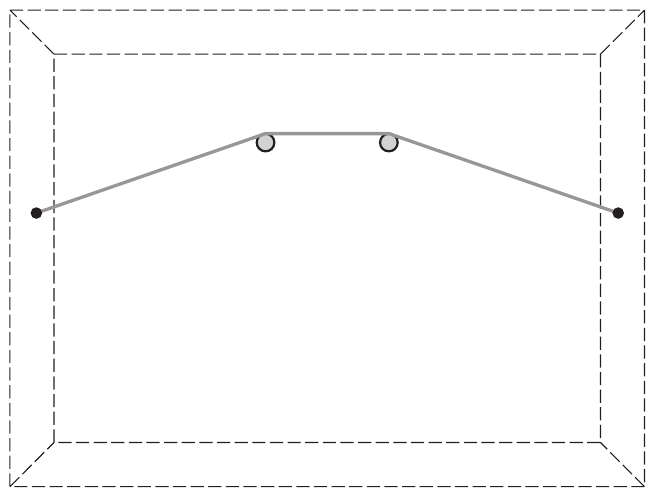
\includegraphics[scale=0.5]{pics/kartina1}
\caption{Эта картина останется висеть если выпадет любой из гвоздей.}
\label{pic:kartina1}
\end{figure}

\subsection*{Замок с дефектом}\rindex{Замок с дефектом}\label{Замок с дефектом}

Кодовый замок имеет три диска, с положениями пронумерованными от 1 до 8.
У замка есть дефект: чтобы его открыть, достаточно правильно выставить два числа из трёх.
Какое минимальное число (трёхзначных) комбинаций достаточно набрать, чтобы наверняка открыть замок?

\parit{Примечания.}
Есть много способов проделать это $64$-мя тестовыми комбинациями, например, можно перебрать все возможные варианты первых двух дисков или проверить все комбинации, сумма значений которых кратна 8.
Однако каждая тройная комбинация покрывает $22$ возможных случаев, а всего комбинаций $8^3 = 512$.
Поэтому в принципе могло бы хватить и $\lceil 512/22 \rceil = 24$ комбинаций.
То есть истина лежит где-то между $24$ и $64$; вопрос --- где?

\subsection*{Альтернативные кубики}\rindex{Альтернативные кубики}

 
Можно ли изготовить такую пару игральных кубиков, чтобы их суммы вели себя так же, как у пары обычных кубиков?
То есть должно быть два способа выбросить 3, шесть способов выбросить 7, один способ выбросить 12 и так далее.
У кубиков должно быть по шесть граней, и на каждой грани должно быть указано положительное целое число.

\subsection*{Совпадение монет}\rindex{Совпадение монет}

Сонни и Шер\footnote{Сонни и Шер --- популярный в 1970-е годы американский поп-рок дуэт Сонни Боно и его супруги Шер.\pr} играют в следующую игру.
В каждом раунде бросается честная монета.
Перед броском Сонни и Шер одновременно объявляют свои предположения о результате броска.
Они выигрывают раунд, если оба угадали правильно.
Требуется максимизировать долю выигранных раундов, предполагая, что игра идёт долго.

Пока что ответ очевиден --- 50\%: Сонни и Шер договариваются о последовательности предположений (например, всегда говорить «орёл»).
Очевидно, что лучшего им не добиться.

Однако перед началом игры игрокам сообщается, что Шер получит результаты всех бросков монеты заранее, прямо перед первым броском!
У неё есть возможность обсудить стратегию с Сонни заранее, но как только она получит данные о бросках, возможности передавать информацию больше не будет.
Возможно ли им добиться 70\%-й доли выигрышей?

\subsection*{Имена в ящиках}\rindex{Имена в ящиках}\label{Имена в ящиках}

Имена ста заключённых помещают в сто деревянных ящиков, по одному в каждом;
ящики расставляются в ряд на столе в комнате.
Заключённых приводят в комнату поочерёдно;
каждому позволяется заглянуть не более чем в 50 ящиков,
затем он должен покинуть комнату, оставив её в точно том же состоянии, как до прихода, и дальнейшее общение невозможно.

У заключённых есть возможность спланировать свою стратегию заранее, и им это понадобится --- если хотя бы один заключённый не найдёт своё имя, то казнят всех.
Найдите стратегию, вероятность успеха которой превысит 30\%.

\parit{Примечания.} Если каждый заключённый откроет случайный набор из 50 ящиков, то вероятность выжить составит незавидные
\[(\tfrac12)^{100}\z\sim 0{,}0000000000000000000000000000008.\]
Но они могут поступить и хуже --- если все откроют одни и те же 50 ящиков, то их шансы упадут до нуля.
Но тридцать процентов уж совсем недостижимы...
Очень хорошо --- вы поняли задачу!

\section*{Источники и решения}

\subsubsection*{Любовь в Клептопии}

Эта головоломка приводится в книге Саймона Сингха \cite{singh};
я узнал её от Кэролайн Калдербэнк, дочке пары математиков Ингрид Добеки и Роба Калдербэнка.
В решении Кэролайн, Ян отправляет Марии ящик с кольцом внутри, навесив на него один из своих замков.
По получении Мария навешивает свой собственный замок на ящик и отправляет её назад с обоими замками.
Когда Ян получает ящик, он снимает свой замок и отправляет ящик опять Марии; вуаля!

Это решение не просто игра;
на нём основан обмен ключами шифрования в протоколе Диффи — Хеллмана, историческим прорывом в криптографии.

В зависимости от предположений, возможны и другие решения.
Моё любимое было предложено компанией участников конференции
«Ga\-the\-ring for Gardner VII», включая оригамиста Роберта Лэнга.
Для этого Ян должен найти замок, ключ от которого имеет большое отверстие, или по крайней мере, отверстие, которое может быть достаточно увеличено сверлением, чтобы ключ мог быть нацеплен за дужку другого замка.
Ян использует этот второй замок, с упомянутым ключом на его дужке, чтобы запереть пустой ящичек, которую он отправляет Марии.
По прошествии времени, достаточном для пересылки (или возможно, после электронного подтверждения от Марии), он отправляет кольцо в другом ящике, запертой первым замком.
Когда Мария получает ящик с кольцом, она открывает её ключом, прикреплённым к первому ящичку, и получает кольцо.

\subsubsection*{Черви и вода}

Это скорее инженерная головоломка, чем математическая.
Она пришла ко мне от Балинта Вирага из Массачусетского технологического института.

Лори действительно может защититься от червей свесив с потолка большой навес, выходящий далеко за кровать.
Но навес должен загибаться внутрь под себя по краям, создавая кольцевой жёлоб, заполненный водой.
(Поперечный разрез навеса показан на рис. \ref{pic:chervi}.)

\begin{figure}[h!]
\centering
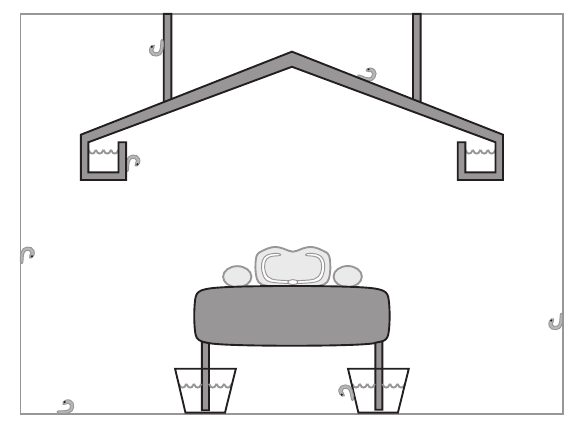
\includegraphics[scale=0.5]{pics/chervi}
\caption{Поперечный разрез Лори в защищённой от червей кровати.}
\label{pic:chervi}
\end{figure}

Если у червей нет способа проникнуть в спальню сверху, то Лори может защититься, обведя комнату по краю жёлобом с водой.

\subsubsection*{Инспекция страусиных яиц}

Вариант этой задачи появился в замечательной книге Джозефа Д. Э. Конхаузера, Дэна Веллемана и Стэна Уэгона \cite{konhauser-velleman-wagon}.

Часто полезно считать данное число (в нашем случае 102) переменной, даже если в конечном счёте нас интересует лишь одно значение.
Пусть $f(k)$ --- максимальное число этажей, которые можно проверить не более чем за $k$ бросков, имея вначале два яйца.
Таким образом, $f(1) = 1$ (прочность яйца может быть $0$ или $1$).
Предположим, что Оскару разрешено сделать $k$ бросков, и он делает первый с $n$-го этажа.
Если яйцо разбилось, то Оскару придётся бросить единственное оставшееся яйцо с 1-го этажа, затем с 2-го и так далее до $(n-1)$-го в худшем случае;
так что $n = k$ это наилучший вариант.
Если яйцо пережило падение с $k$-го этажа, то придётся проверить все этажи выше оставшимися $k-1$ броском (используя два яйца).
Следовательно, $f(k - 1) + k$ это максимальное число этажей, которые можно обработать,
и мы получили рекурсию $f(k) = f(k - 1) + k$.

Прямым вычислением получаем, что $f(2) = 3$, $f(3) = 6$, $f(5) = 10$ и так далее; в общем случае $f(k)$ равно сумме чисел от $1$ до $k$.
Поскольку таких чисел $k$, а их среднее равно $(k + 1)/2$, их сумма (иногда называемая «$k$-ым треугольным числом»), составляет $k(k + 1)/2$.
Первое значение $f(k)$, достигающее 102, это $f(14) = 14 \times 15/2 = 105$, то есть в худшем случае Оскару понадобится $14$ бросков.
Рекурсия указывает и на то как это сделать;
в нашем случае, трёхэтажный запас позволяет Оскару сбросить первое яйцо с одиннадцатого, двенадцатого, тринадцатого или четырнадцатого этажа.
Любой другой вариант может потребовать лишнего броска.

Давайте посмотрим, что происходит с тремя яйцами.
Определим $g(k)$ как максимальное число этажей, которые можно обработать $k$ бросками, начиная с трёх яиц.
Теперь Оскару нужно обработать $g(k \z- 1)$ этажей выше уровня первого броска, если яйцо переживёт падение;
или же $f(k - 1)$ этажей ниже этого уровня (тот же $f$, что и выше), потому что теперь у него лишь два яйца.
Получаем новую рекурсию: $g(k) = g(k-1) + 1 + (k - 1)k/2$, что даёт $g(2) = 3$ (пока без улучшений), но $g(3) = 7$.
В общем случае получаем $g(k)=k(k^2+5)/6$ и наименьшее значение $k$, для которого 
$g(k)\ge 102$, равно $9$.
То есть, если у Оскара есть три яйца,
то ему потребуется максимум девять бросков чтоб обработать Эмпайр-стейт-билдинг.

В общем случае, если $k$ велико, то число этажей, которые можно обработать, имея вначале $m$ яиц, равно $k^m/m!$ плюс члены низших порядков.
Отсюда следует, что с $m$ яйцами и небоскрёбом в $n$ этажей, где  $n$ намного больше $m$, число бросков, необходимых в худшем случае, будет около $(m!\times n)^{1/m}$.

\subsubsection*{Опасная картина}

Эту интересную головоломку предложил Джулио Дженовезе, аспирант в Дартмуте, который узнал её из нескольких источников в Европе.

Один из способов повесить картину изображён на рис. \ref{pic:kartina2}, с зазором, чтобы можно было в нём разобраться.
Шнур проходит над первым гвоздём,
далее идёт петля вокруг второго,
проходит опять над первым гвоздём, и затем снова петля вокруг второго гвоздя, но на этот раз с половинным поворотом.

\begin{figure}[h!]
\centering
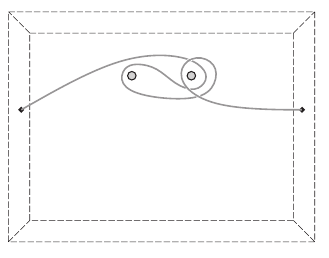
\includegraphics[scale=1]{pics/kartina2}
\caption{Эта картина упадёт если выскочит любой из двух гвоздей.}
\label{pic:kartina2}
\end{figure}

Существуют также некоторые нетопологические решения: например, можно сдавить петлю между двумя близко расположенными гвоздями, предполагая, что ширина головки гвоздя не намного больше толщины шнура.
Но зачем полагаться на трение, когда можно использовать математику?

\begin{addedbytheeditors}
Попробуйте повесить картину на $n$ гвоздей так, чтобы она упала если выскочит любой из них.
А можно ли повесить так, чтоб картина осталась висеть при выпадании одного гвоздя, но падала при выпадании двух?
Хороший обзор подобных задач дан в \cite{demaine2014}, но он не включает результата из \cite{gartside-greenwood}, дающего наилучий способ решения задачи с $n$ гвоздями (без заузливания шнура).
\end{addedbytheeditors}

\subsubsection*{Дефективный кодовый замок}

Этот шедевр комбинаторики достался мне от Амит Чакрабарти из Дартмута;
он был предложен Восточной Германией для Международную математическую олимпиаду 1988 года.

Задачи такого рода лучше решать геометрически.
Пространство всех комбинаций представляет собой комбинаторный куб $8 \times 8 \times 8$.
Каждый раз, когда мы проверяем точку куба, мы вычёркиваем все точки на трёх её координатных линиях.

Представив задачу таким способом, должно быть видно, что лучший способ вычеркнуть все точки это брать все тестовые точки в двух противоположных осьмушках $4 \times 4 \times 4$ нашего куба.
Так можно догадаться до следующего решения.

Давайте проверим все комбинации с числами из $\{1, 2, 3, 4\}$, сумма которых кратна $4$.
Их всего шестнадцать, так как если вы выбираете числа на первых двух (или любых двух) дисках, то число на третьем определяется однозначно.
Теперь попробуем те же комбинации, добавив $(4,4,4)$, то есть, добавив $4$ к каждому из трёх чисел;
их ещё $16$, и мы утверждаем, что вместе эти $32$ комбинации вычёркивают все.

Проверка довольно лёгкая.
Правильная комбинация должна иметь либо два (или более) числа из $\{1, 2, 3, 4\}$, либо два или более числа из  $\{5, 6, 7, 8\}$.
В первом случае положение третьего диска единственно (это число в правильной комбинации может не входить в $\{1, 2, 3, 4\}$), так что получена тройка среди первых $16$ тестовых комбинаций.
Второй случай аналогичен.

А вот способ Амита (есть и другие), объясняющий, что нельзя обойтись $31$-й или менее тестовой комбинацией.
Предположим, что $S$ --- это покрытие, и $|S| = 31$.
Пусть $S_i = \{\,(x, y, z) \z\in S : z = i\,\}$ будет $i$-м уровнем $S$.

Рассмотрим три множества:
$A=\{1, 2, 3\}$,
$B = \{4, 5, 6, 7, 8\}$,
и $C \z= \{2, 3, 4, 5, 6, 7, 8\}$.
По крайней мере, один уровень $S$ должен содержать три или меньше точек;
можно считать, что это $S_1$, и $|S_1| = 3$.
(Если $|S_1| \le 2$, то дойти до противоречия ещё проще.)
Точки $S_1$ должны лежать в некотором $3 \times 3 \times 1$ подкубе;
можно считать, что они лежат в $A \times A \times {1}$.

Заметим, что $25$ точек в $B \times B \times \{0\}$ должны быть вычеркнуты точками, не входящими в $S_1$.
Никакие две из них не могут быть вычеркнуты одной точкой в $S$.
Следовательно, $S - S_1$ содержит подмножество $T$ размером $25$, которое лежит в подкубе $B \times B \times C$.
Теперь рассмотрим множество $P = \{\,(x, y, z) : z \in C, (x, y, 1) \notin S_1 , (x, y) \notin B \times B\,\}$.
Легко подсчитать, что $|P| = (64-3-25) \times 7 = 252$.
Точки в $P$ не вычёркиваются $S_1$, и каждая точка в $T$ может вычеркнуть не более $3 + 3 = 6$ точек в $P$. Следовательно, есть по крайней мере $252 - 6 \times 25 = 102$ точки в $P$, которые должны быть вычеркнуты точками в $S - S_1 - T$.

Однако осталось всего $|S - S_1 - T | = 31 - 3 - 25 = 3$ тестовых точек, и каждая из них вычёркивает ровно $22$ точки.
Поскольку $22 \times 3 = 66 \z< 102$, приходим к противоречию. 

\subsubsection*{Альтернативные кубики}

Эта задача настолько известна, что у её решение есть имя: «кубики Шихермана».
В заметке Мартина Гарднера 1978 года \cite{gardner1978} или в ego книге \cite{gardner1989} можно узнать об их открытии полковником Джорджем Шихерманом, сейчас проживающим в Уэйсайд, Нью-Джерси.
Единственная пара кубиков Шихермана имеет метки $\{1, 3, 4, 5, 6, 8\}$ и $\{1, 2, 2, 3, 3, 4\}$.

Возможно, вы нашли ответ перебором, и это вполне подходящий способ решения.
Однако есть и другой способ, иллюстрирующий мощный математический инструмент --- \emph{производящие функции}.

Идея в том, чтоб сопоставить кубику многочлен от переменной $x$, в котором коэффициент при $x^k$ равен числу граней кубика с меткой $k$.
Обычный кубик, например, будет соответствовать многочлену $f(x) = x \z+ x^2 \z+ x^3 \z+ x^4 \z+ x^5 \z+ x^6$.

Ключевое наблюдение заключается в том, что результат броска двух (или более) кубиков представлен произведением их многочленов.
Например, если мы бросаем два обычных кубика, то коэффициент $x^{10}$ в произведении (то есть в $f(x)^2$) есть число способов выбора двух членов из $f(x)$, произведение которых равно $x^{10}$ ---
это $x^4 \times x^6$, $x^5 \times x^5$ и $x^6 \times x^4$; они представляют три способа получить сумму $10$.

Следовательно, если $g(x)$ и $h(x)$ --- многочлены наших кубиков, то $g(x) \times h(x) = f(x)^2$.
Многочлены, как и числа, единственным способом разлагаются на простые сомножители;
многочлен $f(x)$ разлагается как $x(x + 1)(x^2 + x + 1)(x^2 - x + 1)$.
Чтобы получить произведение $g(x)$ и $h(x)$ равное $f(x)^2$, нам нужно взять каждый из этих $4$ сомножителей и добавить по одной его копии в $g(x)$ и в $h(x)$, или же две его копии в один либо в другой.
Но есть следующие ограничения:
в полученных многочленах $g(x)$ и $h(x)$ не может быть свободных членов (это бы означало, что некоторые стороны помечены нулём);
не допускаются отрицательные коэффициенты;
также сумма коэффициентов в каждом из этих многочленов должна равняться 6.


Единственный решение (кроме $g(x) = h(x) = f(x)$) это
\[g(x)
=
x(x + 1)(x^2 + x + 1)
=
x + 2x^2 + 2x^3 + x^4\]
и
\[h(x)
=
x(x + 1)(x^2 + x + 1)(x^2 - x + 1)^2
=
x + x^3 + x^4 + x^5 + x^6 + x^8,\]
или наоборот.

Мы всё ещё использовали перебор, но таким методом можно решать задачи посложнее.
Во-первых, можно придумать альтернативы для пары восьмигранных игральных костей, пронумерованных от $1$ до $8$ (есть три альтернативных варианта), или для бросания трёх обычных кубиков (много способов).

Читателям, которые хотят поглубже изучить эту тему, стоит обратиться к отличной статье Джо Галлиана и Дейва Русина \cite{gallian-rusin}.

\subsubsection*{Совпадение монет}

Эту задачу предложил мне Одед Регев, из Техниона, в Израиле.
Сонни и Шер могут выиграть более чем в 2/3 случаев.
Для этого разделим последовательность бросков на блоки по три.
Перед каждым блоком Шер \emph{оповещает} Сонни, будут ли в следующем блоке в основном орлы или решки;
если первое, Сонни говорит «ООО» в этом блоке; если второе, то «РРР».

Но как Шер передать эту информацию?
Чаще всего Сонни ошибается (в точности) раз в блоке.
Перед этим броском Шер говорит «О», сообщая, что в следующем блоке будут в основном орлы, и «Р» в противном случае.
Для двух других бросков в текущей тройке Шер даёт правильный ответ (вместе с Сонни), гарантируя две из трёх побед.
Если случится, что Сонни может угадать все три броска в текущей тройке,
то один раз --- скажем на последнем броске, Шер действует, как описано выше, даже если это стоит им потери одной победы.
Таким образом, после первого блока Сонни и Шер будут набирать две победы из трёх, когда блок состоит из двух орлов и одной решки или двух решек и одного орла.
Когда блок состоит полностью из орлов или полностью из решек (что происходит с вероятностью 1/4), они получают две победы из трёх в половине случаев и три из трёх в остальной половине.
Значит доля успеха составит $3/4 \times 2/3 + 1/4 \times 5/6 = 17/24 > 70.8\%$.
Обратите внимание, что даже в наихудшем случае (например, если последовательные орлы и решки выбираются противником, а не случайны) этот метод гарантирует долю успеха хотя бы $2/3$.

Оливье Госснер, Пенелопа Эрнандес и Абрахам Нейман \cite{gossner} доказали, что с более сложными версиями этой схемы Сонни и Шер могут приблизиться к любой доле успеха равной $x$, где $x$ --- единственное решение уравнения
\[-x \log_2 x - (1 - x) \log_2 (1 - x) + (1 - x) \log_2 3 = 1,\]
и лучшего добиться нельзя.
Более того, это утверждение остаётся верным независимо от того, случайны ли броски монеты или нет!
Поскольку это значение $x$ составляет около $0{,}8016$, Сонни и Шер могут на самом деле добиться победы более чем в $80\%$ случаев, даже если оппонент играет против них.

\subsubsection*{Имена в ящиках}

У этой головоломки короткая, но увлекательная история.
Она придумана датским специалистом по информатике Петером Бро Милтерсеном;
её версия появилась в завоевавший широкое признание статье, написанной им и Анной Галь \cite{gal-miltersen}.
Однако Милтерсен не знал  решения, пока его коллега Свен Скиум не указал ему на это во время обеда.
В конечном итоге головоломка дошла до меня (в несколько усложнённой форме) через Дорит Ахаронов.

Чтобы её решить, заключённые должны сначала договориться о случайном соответствии ящиков со своими именами.
(Это сделает невозможным разложить имена в ящиках так, чтобы помешать протоколу, описанному ниже.)
Попадая в комнату, каждый заключённый проверяет свой собственный ящик (то есть ящик, с которому соответствует его имя).
Затем он заглядывает в ящик, соответствующий имени, которое он только что нашёл,
затем в ящик, соответствующий имени, найденному во втором ящике, и так далее, пока он не найдёт своё собственное имя или не откроет 50 ящиков.

Вот такая стратегия, но почему она работает?
Соответствие, между именем владельца ящика и именем, найденном в его ящике, представляет собой перестановку из 100 имён, выбранную равномерно случайным образом из набора всех таких перестановок.
Каждый заключённый идёт по циклу перестановки, начиная со своего имени.
Если цикл не длиннее 50, то он находит своё имя.
Если перестановка не длинней 50, то это сработает для всех, и заключённые будут спасены.

Вероятность того, что равномерно случайная перестановка чисел от $1$ до $2n$ не содержит ни одного цикла длиной более $n$, равна по крайней мере, $1$ минус натуральный логарифм от $2$, что составляет около $30,6853\%$.

Чтобы увидеть это, положим $n < k \le 2n$ и сосчитаем перестановки, имеющие цикл $C$ длиной ровно $k$.
Есть $\binom{2n}k$ способов выбрать имена в этом цикле, $(k - 1)!$ способов упорядочить их в $C$
и $(2n - k)!$ вариантов перестановки остальных имён;
произведение этих чисел равно $(2n)!/k$.
Поскольку в данной перестановке не более одного $k$-цикла, вероятность того, что такой имеется, в точности равна $1/k$.
Значит вероятность отсутствия длинного цикла равна
\[1-\frac{1}{n}-\frac{1}{n+1}-\dots-\frac{1}{2n}=1-H_{2n}-H_n\]
где $H_m$ --- сумма обратных чисел первых $m$ положительных целых чисел, что приблизительно равно $\ln m$.
Таким образом, наша вероятность будет близка к $1 - \ln 2n + \ln n = 1 - \ln 2$, на самом деле всегда чуть больше этого значения.
Для $n = 50$ мы получаем, что заключённые выживают с вероятностью $31,1827821\%$.
Недавно Юджин  Кертин и Макс Варшауэр \cite{curtin-warshaue} показали, что это решение нельзя улучшить.

Ламберт Брайт и Рори Ларсон, а также независимо Ричард Стэнли из Массачусетского технологического института, предложили следующую вариацию.
Предположим, что каждый заключённый должен заглянуть в \emph{не менее} чем 50 ящиков, и требование для выживания заключается в том, чтобы каждый заключённый \emph{не} нашёл собственное имя?
Несмотря на то, что цель полностью противоположна, похоже, что у заключённых нету лучшего варианта чем как следовать точно той же стратегии.
Однако теперь они выживают лишь, если каждый цикл длиннее $50$, а это происходит только при наличии единственного большого цикла длины $100$ --- шансы составляют ровно $1$ к $100$.
Не очень обнадёживает, но всё же лучше, чем $1$ к $2^{100}$.

Заметим, что у заключённых будут те же шансы, если каждому потребуется заглянуть в $99$ ящиков --- снова они следуют стратегии и выигрывают если случайная перестановка является циклом.
В этом случае сразу очевидно, что лучшей стратегии нет.
Ведь самый первый заключённый, чтобы он не делал, выживет с вероятностью $1\%$.
Забавно, что, если следовать этой стратегии, то как только повезло первому заключённому, так автоматически везёт всем остальным!

\chapter{Числовые загадки}


\setlength{\epigraphwidth}{.85\textwidth}
\epigraph{У творца вселенной таинственный образ действий.
Но он использует десятичную систему счисления и любит круглые
числа.
}{--- Скотт Адамс (1957---)}


Свойства чисел --- странная и прекрасная штука, и неудивительно, что на них основано много замечательных головоломок; иногда они даже помогают нам кое-что понять о самих числах.

\subsection*{Строки и столбцы}

Докажите, что если упорядочить каждую строку матрицы, а затем каждый столбец, то строки останутся упорядоченными!

\subsection*{Нежелательное раскрытие}

Дано алгебраическое выражение с переменными, сложением, умножением и скобками.
Вы рекурсивно раскрываете скобки, используя распределительный закон умножения.
Как убедиться, что этот процесс не будет продолжаться вечно?

\parit{Примечания.}
Может показаться, что число скобок должно уменьшаться.
Однако если раскрыть первые скобки в
\[(x + y)(s(u + v) + t),\]
то получим выражение
\[x(s(u + v) + t) + y(s(u + v) + t),\]
с б\'{о}льшим числом скобок.

\subsection*{Хамелеоны}\label{Хамелеоны}

На острове живут 20 красных, 18 синих и 16 зелёных хамелеонов.
Если встречаются два хамелеона разных цветов, то каждый из них меняет свой цвет на оставшийся третий.
Может ли случиться так, что через некоторое время все хамелеоны будут одного цвета? 

\subsection*{Отсутствующая цифра}

Число $2^{29}$ состоит из $9$ различных цифр; какая цифра отсутствует?

\subsection*{Очень честное разбиение}

Можно ли разбить целые числа от $1$ до $16$ на два набора одинакового размера так,
чтобы у них были равные суммы, равные суммы квадратов и равные суммы кубов?

\subsection*{Восстановление чисел}
Для каких положительных целых чисел $n$ верно следующее: зная все $\binom n2$ попарных сумм $n$ различных положительных целых чисел, всегда можно однозначно восстановить сами числа?


\subsection*{Уравнение ирисок}

$n$ детей стоят кружком и каждый держит несколько ирисок.
Учитель даёт дополнительную ириску каждому ребёнку, у которого их нечётное число,
затем каждый ребёнок передаёт половину своих ирисок ребёнку слева от себя.
Эта пара процедур повторяется, до тех пор пока они уже ничего не меняют.
Докажите, что этот процесс действительно завершится, и у всех детей будет по одинаковому (чётному) числу ирисок.

\subsection*{Девяносто девятая цифра}

Какая цифра стоит на 99-м месте после запятой в десятичном разложении числа 
$(1+\sqrt2)^{500}$?

\subsection*{Подмножества с ограничениями}

Каково максимальное число целых чисел от $1$ до $30$, произведение любой пары которых не является полным квадратом?
А что если (вместо этого) ни одно число не кратно другому?
Или, ни у какой пары нет общего делителя (отличного от 1)?

\subsection*{Единообразие бубликов}\label{Единообразие бубликов}

Чёртова дюжина (то есть 13 штук) бубликов обладают таким свойством: любую дюжину из них можно разделить на две кучки по шесть, которые в точности уравновесят друг друга на весах.
Докажите, что все 13 бубликов одинакового веса.

\medskip

Следующая головоломка сложней большинства остальных;
она включена по особой причине.

\subsection*{Юбилейная головоломка}

Поскольку ряд $1 - 1 + 1 - 1 + 1 - \dots$ не сходится,  функция 
$f(x)\z=x-x^2+x^4-x^8+x^{16}-x^{32}+\dots$ не определена при $x=1$.
Однако $f(x)$ сходится при всех положительных вещественных чисел $x<1$.
Сходится ли $f(x)$ при $x$ стремящимся к 1 снизу?

\subsection*{Надёжные мигалки}\label{Надёжные мигалки}

Две обычные мигалки мигают одновременно в момент времени $0$
и мигают дальше; при этом у них вместе \emph{в среднем} получается по одному миганию в минуту.
Известно, что они больше никогда не мигнут одновременно (или, что то же самое, отношение их частот иррационально).

Докажите, что после первой минуты (во временном интервале между $0{:}00$ и $0{:}01$) в каждом интервале между $t$ и $t + 1$ минутой будет ровно одно мигание ($t$ --- натуральное число).

\subsection*{Красные и синие игральные кости}\label{Красные и синие игральные кости}

У нас есть два набора (красный и синий) из $n$ игральных костей с $n$ гранями на каждой;
на гранях каждой кости стоят числа от $1$ до~$n$.
Мы бросили все $2n$ костей одновременно.
Докажите, что можно выбрать непустое подмножество красных и непустое подмножество синих костей с одинаковой суммой!

\section*{Источники и решения}

\subsubsection*{Строки и столбцы}

Это классическая теорема, простая и удивительная; о ней мне напомнил Дэн Ромик, сейчас он в Иерусалимском университете.
В третьем томе своего «Искусства программирования» \cite{41} Дональд Кнут проследил историю этого результата до сноски в книге 1955 года Германа Бёрнера \cite{7}.
Бриджет Теннер, студентка знаменитого комбинаторика Ричарда Стэнли из Массачусетского технологического института, недавно обобщила эту теорему \cite{57}.
Теорема Бёрнера --- одна из тех задач, где таинственность и очевидность чередуются при каждой попытке найти решение.

Предположим, что у матрицы $m$ строк и $n$ столбцов.
Положим, что $a_{ij}$ --- значение в $i$-й строке и $j$-м столбце матрицы
после упорядочивания каждой строки (будем считать, что самые маленькие значения находятся слева).
Обозначим через $b_{ij}$ значение в той же клетке матрицы после упорядочивания столбцов.

Нужно показать, что $b_{ij} \le b_{ik}$ если $j < k$.
Заметим, что $b_{ik}$ это $i$-й наименьший элемент в старом столбце $\{a_{1k}, a_{2k}, \dots, a_{mk}\}$.
Далее, $a_{i'j}\le a_{i'k}$ поскольку $a_{i'j}$ стоит левее $a_{i'k}$ в той же строке.
В частности, если $a_{i'k}\le b_{ik}$, то $a_{i'j}\le b_{ik}$.
Значит есть как минимум $i$ элементов из старого $j$-го столбца, которые не превосходят $b_{ik}$,
и в частности, $i$-й наименьший элемент в старом $j$-м столбце не превосходит $b_{ik}$;
то есть, $b_{ij} \le b_{ik}$ --- конец доказательства.

Может было б убедительней разобрать конкретный пример?
Решайте сами.


\begin{addedbytheeditors}
\textbf{Редакторам:} Перетащил одну фразу из одного абзаца в другой.
\end{addedbytheeditors}

\subsubsection*{Нежелательное раскрытие}

Эту любопытную головоломку мне подкинул Ричард Липтон с компьютерного колледжа Технологического института Джорджии.
Есть решение с использованием глубины дерева, но есть и более простой способ:
установите все переменные равными 2!
Поскольку применение закона дистрибутивности не меняет значения выражения, получаем ограничение на длину любого выражения, которое можно получить из него, раскрывая скобки.

\subsubsection*{Хамелеоны}

Борис Шейн, алгебраист из Университета Арканзаса, прислал мне эту головоломку; она может быть довольно древней.
Мне известен случай, когда её дали ученику восьмого класса в Харькове,
и ещё другой, когда её дали выпускнику Гарварда, проходившему собеседование в крупной финансовой фирме;
оба с ней справились!

Главное увидеть, что после каждой встречи разница между числом особей любых двух цветов не меняется по модулю~3.
Обозначим через $N_{\text{к}}$ число красных хамелеонов, и пусть
$N_{\text{с}}$ и $N_{\text{з}}$ --- число синих и зелёных.
Мы утверждаем, что, например, у разницы $N_{\text{к}} - N_{\text{с}}$ не меняется остаток при делении на~$3$ после каждой встречи хамелеонов.
В этом можно убедиться, проверив случай за случаем.
Таким образом, эти разницы остаются одинаковыми по модулю 3 навсегда, и поскольку ни одна из этих разниц не равна нулю по модулю 3, нам не удастся избавиться от двух цветов.

С другой стороны, если одна из этих разниц (скажем, $N_{\text{к}} - N_{\text{с}}$) является положительным кратным $3$, то её можно уменьшить, заставив красного хамелеона встретиться с зелёным (если зелёных нет, то придётся сначала заставить красного встретиться с синим).
Повторив это несколько раз, можно добиться, что $N_{\text{к}} = N_{\text{с}}$.
Затем заставим красных хамелеонов встречаться с синими, пока не останутся только зелёные.
Собрав всё воедино и отметив, что если две разницы кратны $3$, то и третья кратна $3$, мы увидим, следующее:
\begin{itemize}
\item если все три разницы кратны 3, то любой цвет может захватить остров;
\item если только одна из разниц кратна 3, то оставшийся цвет --- единственный, который может захватить остров; и наконец,
\item если ни одна из разниц не кратна 3, как в данной задаче, то все хамелоны не смогут стать одноцветными до тех пор, пока не вмешаются другие обстоятельства (например, рождение или смерть).
\end{itemize}

Эта головоломка была предложена осенью 1984 года на Турнире городов (с числами 13, 15 и 17) как задача 5 в подготовительном варианте для 9--10 классов и основном варианте для 7--8 классов.
Турнир городов, из которого дальше будет больше задач, был основан в 1980 году Николаем Константиновым из Москвы.
В то время начиналась перестройка и гласность, это затронуло и математические олимпиады, как и все другие аспекты советской жизни.
Константинов был недоволен определёнными переменами, вышел из жюри Всесоюзной олимпиады и сам организовал турнир для маленьких городов в сельской России.
Он собрал вокруг себя замечательных математиков, и успех турнира в конечном итоге привёл к тому, что Москва сама стала одним из «городов».
Эта же группа основала Независимый московский университет в 1993 году.
Сама же группа превратилась в МЦНМО.

Турнир распространился в Польшу и Болгарию.
В 1989 году, благодаря усилиям Питера Тейлора из Университета Канберры, был проведён в Австралии.
В настоящее время Тейлор является исполнительным директором Австралийского математического фонда, под его эгидой он выпустил пять книг о турнире.

В 1990 году Энди Лиу привёз Турнир в Канаду.
С тех пор он распространился по всему миру, с участниками из Соединённых Штатов, Западной Европы, Азии и Южной Америки.
Задачи и решения на английском языке подготавливаются Андреем Сторожевым и Энди Лиу.

\begin{addedbytheeditors}
Автор В. Ильичев.

\textbf{Редакторам:} Вроде история тургора не совсем правда.
\end{addedbytheeditors}

\subsubsection*{Отсутствующая цифра}

Эта забавная загадка взята из колонки головоломок Берлекэмпа и Бюлера в журнале Emissary [3], весна/осень 2006 года,
а они услышали её от теоретика чисел Хендрика Ленстры.
Конечно же можно загуглить ``\texttt{2\^{}29}'' и увидеть число, но как решить эту задачу в уме, без головной боли?

Ну возможно, вы помните технику из начальной школы, так называемое \emph{вычеркивание девяток} --- если сложить все цифры то получим значение числа по модулю 9 (то есть  с тем же остатком при деления на 9).
Этот метод иногда называют индийской или арабской проверкой;
он основан том, что $10 \equiv 1 \pmod 9$, следовательно, $10^n \equiv 1^n \equiv 1 \pmod 9$ для любого $n$.
Если обозначить через $x^*$ сумму цифр числа $x$, то получим $(xy)^* \equiv x^* y^* \pmod 9$ для любых $x$ и $y$.
В частности, $(2^n)^* \equiv 2^n \pmod 9$.
Остатки от деления степеней числа $2$ на $9$ начинаются с $2$, $4$, $8$, $7$, $5$, $1$, и зацикливаются;
так как $29 \equiv 5 \pmod 6$, получаем, что $2^n \pmod 9$ есть пятое число этой последовательности, то есть $5$.
Теперь сумма всех цифр равна $10 \times 4{,}5 = 45 \equiv 0 \pmod 9$, поэтому пропущенная цифра должна быть четвёрткой.
И действительно, $2^{29} = 536\,870\,912$.

\subsubsection*{Очень честное разбиение}

Мне эту головоломку подбросил Муту Мутукиршнан (Рутгерс),
а сам он узнал её от Боба Тарджана (Принстон);
оба они выдающиеся специалисты по информатике.

Оказывается, есть такое разбиение: $\{1$, $4$, $6$, $7$, $10$, $11$, $13$, $16\}$ и $\{2$, $3$, $5$, $8$, $9$, $12$, $14$, $15\}$.

Чтобы догадаться как его строить, можно подумать:
а ведь $16$ это степень двойки;
может попытаться обобщить?
Можно ли, например, разбить числа от $1$ до $8$ на две равные части с одинаковой суммой и суммой квадратов?
А как насчёт разделения чисел от $1$ до $4$ на две равные части с одинаковой суммой?
Последнее сделать легко: $\{1, 4\}$ и $\{2, 3\}$.
Заметим, что $\{5, 8\}$ и $\{6, 7\}$ разбивают числа от $5$ до $8$ и решает ту же задачу.
Если соединить эти два разбиения крест-накрест, то получим $\{1, 4, 6, 7\}$ и $\{2, 3, 5, 8\}$, по построению оно подходит для сумм, но вроде бы подходит и для сумм квадратов.

В общем случае, пользуясь индукцией, можно доказать, что числа от $1$ до $2^k$ можно разбить на множества $X$ и $Y$ так, что каждая часть имеет одинаковую сумму $j$-х степеней, где $j$ меняется от $0$ до $k - 1$, и, значит $p(X)=p(Y)$ для любого многочлена $p$ степени меньше $k$;
где $p(X)$ определятся как сумма всех значений $p(x)$ при $x \in X$.

Чтобы перейти от $2^{k}$ к $2^{k+1}$, возьмём $X' = X \cup (Y + 2^k)$
(где $Y + 2^k$ получается из $Y$ добавлением $2^k$ к каждому элементу) и $Y' \z= Y \cup (X + 2^k)$.
Заметим, что $p(X + 2^k) = p(Y + 2^k)$,
так как $p(X + 2^k)=q(X)$ и $p(Y + 2^k)=q(Y)$ для некоторого другого многчлена $q$ той же степени.
Таким образом, $X'$ и $Y'$ согласуются для многчленов степени меньше $k$, ну а что если наш многочлен $r$ степени $k$?

Но и здесь всё в порядке, ведь старшие члены в $r(x+2^k)$ и $r(x)$ совпадают;
то есть $s(x)=r(x+2^k)-r(x)$ есть многочлен степени меньше $k$.
Таким образом,
\begin{align*}
r(X')&=r(X)+r(Y+2^k)=r(X)+r(Y)+s(Y),
\\
r(Y')&=r(Y)+r(X+2^k)=r(Y)+r(X)+s(X).
\end{align*}
Поскольку $s(Y)=s(X)$, получаем, что $r(X')\z=r(Y')$.

Эта задача напрямую связана с так называемым \emph{многостепенном уравнением}.
Основной вклад в его изучение внёс Альберт Гроден в своей монографии \cite{gloden}.


\begin{addedbytheeditors}
\textbf{Редакторам:} Я расширил параграф «Но здесь...».
\end{addedbytheeditors}

\subsubsection*{Восстановление чисел}

Эту головоломку прислал мне Ник Райнгольд из AT\&T Labs.
Ответ таков: это возможно тогда и только тогда, когда $n$ не является степенью двойки!
И мы снова применим силу многочленов.

Предположим, что $X = \{x_1 , \dots , x_n\}$ и $Y = \{y_1 , \dots , y_n\}$ --- два различных множества с одинаковыми попарными суммами.
Пусть $p(z)$ --- многочлен $z^{x_1} + z^{x_2} + \dots + z^{x_n}$,
а $q(z)$ --- многочлен $z^{y_1} + z^{y_2} + \dots + z^{y_n}$.
По условию, смешанные члены в $p(z)^2$ те же, что и в $q(z)^2$;
то есть,
\[p(z)^2 -q(z)^2 = p(z^2 )-q(z^2).\]
Разделив равенство на $p(z) - q(z)$, получим
\[p(z) + q(z) =
\frac{p(z^2 ) - q(z^2 )}{p(z) - q(z)}.
\]
Поскольку $p(1) = q(1) = n$,
у многочлена $p(z) - q(z)$ есть корень $1$ с некоторой положительной кратностью $k$.
Значит
\[p(z) - q(z) = (z - 1)^k r(z).\]
Точно также получаем
\[p(z^2 ) - q(z^2 ) = (z^2 - 1)^k r(z^2 )= (z - 1)^k (z + 1)^k r(z^2).\]
Сократив дробь на $(z - 1)^k$, получаем
\[p(z) + q(z) =
\frac{(z + 1)^k r(z^2)}{r(z)}.
\]
Подставив $z = 1$, получаем $2n = 2^k$ --- полдела сделано!

Остаётся показать, что если $n$ степень двойки, то
числа не всегда можно восстановить.
Для этого воспользуемся множествами $X$ и $Y$ из предыдущей задачи.
Предположим, что $\{1, \dots , 2^k\}$ разбиты на подмножества $X$ и $Y$ с теми же парными суммами.
Рассмотрим $X' = X \cup (Y + 2^k)$ и $Y' = Y \cup (X + 2^k)$.
Парные суммы $X'$ имеют вид $x_1 + x_2$, $y_1 + y_2 + 2^{k+1}$ и $x + y + 2^k$.
По предположению индукции,
суммы $x_1 + x_2$, те же, что и $y_1 + y_2$.
Значит, попарные суммы из $Y'$ точно те же, что и из $X'$.

\begin{addedbytheeditors}
Про пример можно думать геометрически.
Если $X$ и $Y$ --- множества чётных и нечётных вершин $k$-мерного параллелепипеда, то легко видеть, что все середины диагоналей с вершинами в $X$ те же, что с вершинами в $Y$.
Остаётся спроектировать параллелепипед на прямую так чтоб все вершины попали в целые числа.
\end{addedbytheeditors}

\subsubsection*{Уравнение ирисок}

Эта задача была представлена Клиффом Смитом (Массачусетский технологический институт) на прекрасном сайте головоломок «The Puzzle Toad» \cite{bohman-pikhurko-frieze-sleator}, который ведут Том Боман, Олег Пихурко, Алан Фриз и Дэнни Слейтор в Университете Карнеги — Меллона.
Она появилась на Пекинском математическом соревновании старших классов 1962 года (12 класс, лист II, задача 4).

Пусть $M$ --- максимальное число ирисок у одного из детей в данный момент времени.
Заметим что число $M$ может увеличиться только если оно нечётное;
в этом случае оно может увеличиться только на единицу до следующего чётного числа.
Чтобы понять это, предположим сначала, что $M$ чётное; тогда оно, конечно же, не изменится, когда учитель раздаёт дополнительные ириски, а после передачи ирисок ни один ребёнок не сможет иметь их больше чем $\tfrac12 M + \tfrac12 M = M$ штук.
Если же $M$ нечётное, то оно увеличится на один до следующего чётного числа, и после этого заработает предыдущее рассуждение.

Значит, рано или поздно, учитель прекратит раздавать ириски.
Теперь наша задача --- показать, что ириски \emph{уравнятся}.

Хороший способ измерить \emph{неравенство} набора из $n$ чисел с фиксированной суммой --- рассмотреть сумму их квадратов; она минимизируется если числа стоят как можно ближе друг к другу.
Давайте рассмотрим этот параметр в нашем случае, а именно 
\[S = G^2_1 + G^2_2 + \dots + G^2_n,\]
где $G_i$ --- число ирисок, у $i$-го ребёнка.
Изменение $S$ после передачи ирисок составит
\begin{align*}
\left(\tfrac{1}{2}(G_n+G_1)\right)^2+\left(\tfrac{1}{2}(G_1+G_2)\right)^2+&\dots+\left(\tfrac{1}{2}(G_{n-1}+G_n)\right)^2-
\\
-G_1^2-G_2^2-&\dots-G_n^2=
\\
=-\tfrac12\bigl((G_n-G_1)^2+(G_1-G_2)^2+&\dots+(G_{n-1}-G_n)^2\bigr).
\end{align*}
Если есть пара соседей с разным числом ирисок, то это отрицательное целое число (ведь все $G_i$ сейчас уже чётные).
Таким образом, $S$ уменьшается каждый раз при передаче ирисок, пока числа ирисок не уравняться.
Поскольку положительное число $S$ не может бесконечно уменьшаться на целые числа, всё доказано!

\medskip

Тех кто знаком с теорией вероятностей, может заинтересовать, следующее впечатляющее обобщение этой задачи в стиле цепей Маркова.

Пусть $M=\{p_{ij}\}$ --- матрица перехода эргодической цепи Маркова с конечным числом состояний, и все $p_{ij}$ рациональны.
Если в конце раунда у $i$-го ребёнка $m_i$ ирисок,
то учитель раздает ириски так, чтобы у $i$-го ребенка стало $n_i$ ирисок, где $n_i$ --- наименьшее число, не меньшее  $m_i$ и при этом $p_{ij}n_i$ являлось бы целым для всех $i$ и $j$.
Далее, $i$-й ребёнок передаёт $p_{ij}n_i$ ирисок $j$-му ребёнку.

Верно ли, что этот процесс завершается после конечного числа раундов
(и при этом доля ирисок каждого ребёнка станет пропорциональна стационарному распределению цепи Маркова $\{\pi_i\}$)?
Этот вопрос был поставлен на математическом семинаре в Кембриджском университете примерно в 1975 году моим коллегой из Дартмута Лори Снеллом и решён Ричардом Вебером.

Вебер рассматривает целочисленный вектор $(M_1, \dots , M_n)$ пропорциональный $(\pi_1, \dots , \pi_n)$, такой, что каждая компонента $M_i$ не меньше начального числа ирисок у $i$-го ребёнка.
Далее он замечает, что если $m_i \leqslant M_i$ для всех $i$, то и $n_i \leqslant M_i$, так как пополнение $n_i$ до $M_i$ тоже сработало бы.
Отсюда 
\[m'_j
:=
\sum_i p_{ij} n_i
\leqslant
\sum_i p_{ij} M_i
=
M_j,\] где $m'_j$ --- число ирисок у $j$-го ребенка в конце раунда.
Воспользовавшись индукцией, можно заключить, что число ирисок у $i$-го ребенка никогда не превысит $M_i$.

Остается заметить, что в течение последовательности раундов, когда учитель не раздает ириски, доли ирисок у детей приближаются к стационарному распределению.
А это не может продолжаться вечно, ведь у нас лишь конечное число способов распределить ириски.
Следовательно, ириски добавляются конечное время до тех пор, пока их общее число $S\leqslant\sum_iM_i$ не достигнет некоторого значения, на котором стационарное распределение и будет достигнуто.

\subsubsection*{Девяносто девятая цифра}

Эта загадка взята из журнала Emissary \cite[осень 1999]{3}, и выглядит довольно сложной.
Даже если пользоваться компьютером, понадобится некоторое терпение (или специальная программа).

Вместо этого заметьте, что число
\[(1+\sqrt{2})^{500}+(1-\sqrt{2})^{500}\]
целое.
Ведь после раскрытия скобок, все нечётные степени $\sqrt{2}$ сокращаются.
Второе слагаемое чрезвычайно мало --- поскольку $|1-\sqrt{2}|\z<\tfrac12$, получаем $(\tfrac12)^5<0{,}1$, и, значит, оно гораздо меньше, чем $10^{-100}$ (на самом деле что-то около $4 \times 10^{-192}$).

То есть у $(1+\sqrt{2})^{500}$ не нахватает крошечной величины до целого, и значит его десятичная запись обладает внушительной последовательностью девяток после запятой.
(На самом деле их $191$, и за ними следует $590591051\dots$)
В частности, 99-ой цифрой будет девятка.

Фокус добавления $(1-\sqrt{2})^{500}$ может показаться немного из ниоткуда, но такие пары сопряжённых степеней, одна большая и одна маленькая, часто встречаются в математике.
Известная формула Бине\footnote{Формула Бине была известна Леонарду Эйлеру, она была получена Абрахамом де Муавром (1667---1754), а может быть и раньше него.}
\[F_n=\frac{1}{\sqrt{5}}\left(\frac{1+\sqrt{5}}2\right)^n-\frac{1}{\sqrt{5}}\left(\frac{1-\sqrt{5}}2\right)^n\]
выдаёт точные значения чисел Фибоначчи $1, 1, 2, 3, 5, 8, 13, 21, 34 \dots$
Второе слагаемое в этой формуле настолько мало, что для любого $n \ge 0$ достаточно вычислить
\[\frac{1}{\sqrt{5}}\left(\frac{1+\sqrt{5}}2\right)^n.\]
Округлив полученное число до ближайшего целого, получим в точности $F_n$.

\begin{addedbytheeditors}
\textbf{Редакторам:}
Я убрал следующий абзац --- по-моему он бессмысленный.

Странно, не так ли?
По тому же рассуждению $(1+\sqrt{2})^{502}$ также невероятно близко к целому,
а отношение этих двух огромных степеней равно $(1+\sqrt{2})^{2}$, что равно прозаическому  $5{,}82842712\dots$
\end{addedbytheeditors}

\subsubsection*{Подмножества с ограничениями}

Все три головоломки решаются одним способом.
Первая была представлена давним мастером головоломок Соломоном Голомбом (Университет Южной Калифорнии) на конференции
«Ga\-the\-ring for Gard\-ner VII»;
вторая предложена Прасадом Тетали из Технологического института Джорджии;
третья --- нехитрая её вариация.

Идея в том, чтоб покрыть числа от 1 до 30 группами чисел так, чтобы из каждой группы только одно число можно было бы включить в множество.
При этом если \emph{получится} собрать подмножество с одним элементом из каждой группы, то оно будет максимальным.

В первом случае рассмотрим любое число $k$ без квадратов (то есть его разложение содержит не больше одной копии любого простого числа).
Теперь посмотрим на множество $S_k$, которое получается, умножением $k$ на все возможные квадраты.

Если взять два числа, скажем, $kx^2$ и $ky^2$, из $S_k$, то их произведение будет квадратом: $k^2x^2y^2 = (kxy)^2$.
Поэтому оба числа не могут быть в нашем подмножестве.
С другой стороны, произведение пары чисел из разных $S_k$ не может быть квадратом.
Действительно, если $k_1\ne k_2$, то у одного будет простой делитель, не встречающийся в другом, и этот делитель появится нечётное число раз в разложении их произведения.

\emph{Каждое} число находится только в одном из этих множеств $S_k$;
то есть для данного $n$ есть единственное $k$, что $n \in S_k$.
Число $k$ можно найти, перемножив простые числа, появляющиеся с нечётной степенью в разложении $n$.
Между $1$ и $30$ таких $19$ штук: $1$, $2$, $3$, $5$, $7$, $11$, $13$, $17$, $19$,
$23$, $29$, $2 \times 3$, $2 \times 5$, $2 \times 7$, $2 \times 11$, $2 \times 13$, $3 \times 5$, $3 \times 7$.
Представителем в $S_k$ можно взять само $k$.
Таким образом, подмножество размером $19$ достижимо и наилучшее возможное.

Чтобы избежать деления одного числа на другое без остатка, заметим, что из группы $B_j \z= \{j, 2j, 4j, 8j, \dots\}$ при нечётном $j$ (то есть, $j$ умноженное на всевозможные степени двойки) можно взять только одно число.
Если включить в наше множество верхнюю половину чисел от $1$ до $30$, то есть с $16$ по $30$, то получим по одному представителю из каждого $B_j$, и, конечно, ни одно из этих чисел не делится друг на друга без остатка --- все их отношения меньше $2$.
Таким образом, $15$ полученных чисел составляют наилучшее возможное подмножество.

Наконец, чтобы получить максимальное подмножество попарно взаимно простых, естественно посмотреть на группы из всех кратных фиксированного простого числа $p$.
Представителем такой группы можно взять само $p$. 
И значит лучше, что можно сделать это выбрать все простые числа до $30$, плюс добавить $1$, получится $11$ штук.

\subsubsection*{Единообразие бубликов}

Эта милая головоломка взята с 12-й Московской математической олимпиады 1949 года;
она включена в первую часть «Избранных задач и теорем элементарной математики» %Д. О. Шклярского, Н. Н. Ченцова и И. М. Яглома
\cite[задача 127, стр. 28]{51}.

Предположим, что не все веса одинаковы.
Если все веса целые, то можно прийти к противоречию следующим образом.
Сдвинем веса вниз (это ни на что не влияет), чтобы самый лёгкий бублик стал нулевого веса.
Теперь давайте делить все веса на два до тех пор, пока не останется бублик с нечётным весом.
Если отложить бублик с нечётным весом, то сумма весов оставшихся должна быть чётной, иначе их невозможно было бы уравновесить.
Но то же самое верно, если мы отложим бублик с нулевым весом --- противоречие.

Это рассуждение работает, если все веса рациональны, ведь единицу измерения можно выбрать так, чтобы все веса стали целыми.
Но что, если веса иррациональны?
Кажется заманчивым заменить каждый вес на близкое рациональное число и применить приведённое рассуждение.
Однако эта идея не срабатывает.

Для иррационального случая, мы воспользуемся техникой посерьёзней.
О вещественных числах $\mathbb{R}$ придётся думать как о векторах над рациональными числами $\mathbb{Q}$;
другими словами, будем считать, что каждое вещественное число это сумма некоторого набора чисел, умноженных на рациональные коэффициенты.
Пусть $V$ будет подпространством (конечномерным), порождённым всеми весами бубликов.
Пусть $r$ --- один из членов базиса $V$, а $q_i$ --- рациональный коэффициент при $r$ у веса $i$-го бублика, записанного в нашем базисе.
Воспользовавшись рассуждением для рациональных весов, получаем, что все $q_i$ обнуляются, но это означает, что $r$ не содержится в $V$ --- противоречие.

Кстати, стоит отметить, требование класть по шесть бубликов на чашки весов является необходимым.
В противном случае, можно взять $7$ бубликов по $50$ грамм и $6$ по $70$, и эти $13$ бубликов будут обладать указанным свойством!
Приведённое доказательство разваливается там, где мы сдвигаем все веса;
в этот момент мы использовали, что на каждой чашке весов равное число бубликов.

\begin{addedbytheeditors}
Идея приближения весов всё же срабатывает, но требует дополнительных усилий.
Для этого достаточно найти приближения весов $m_i$ дробями $\tfrac{p_i}q$ так, чтобы следующие неравенства
$|m_i-\tfrac{p_i}q|<\tfrac\varepsilon q$,
выполнялись для всех $i$ и для произвольно малого наперёд заданного $\varepsilon>0$.
Эту оценку следует из теоремы Дирихле о диофантовых приближениях.
Подобным образом можно получить вариацию решения третье проблемы Гильберта \cite[Lemma 1]{benko}. 
\end{addedbytheeditors}


\subsubsection*{Юбилейная головоломка}

Эта недетская головоломка взята из журнала Emissary \cite[Осень 2004]{3}.
Она появилась на свет гораздо раньше, в статье великого английского математика Годфри Х. Харди \cite{37}. 
Харди нашёл правильный ответ, и отметил, что ему неизвестно элементарное доказательство.
К счастью, за последующие 100 лет таковое нашлось.

Ясно, что у Харди не было доступа к компьютеру.
Если бы он попытался вычислять $f(x)$ вручную для различных $x$ близких к $1$, то могло бы показаться, что функция сходится к $1/2$.
Однако, на самом деле предела нет.

Следующее милое доказательство нашёл Ноам Элкис, Гарвардский математик и композитор \cite[Problem 8]{elkies}.
Предположим, что предел есть%
\footnote{Сам Харди однажды сказал: «\emph{Reductio ad absurdum}, так любимое Евклидом, --- одно из лучших оружий математика.
Это гораздо более изощрённый ход, чем любая партия в шахматы:
шахматист может пожертвовать пешку или даже фигуру, а математик жертвует самой игрой».};
поскольку $f(x)\z=x\z-f(x^2)$, он обязан быть равен $1/2$.
Но $f$ также удовлетворяет соотношению $f(x)\z=x\z-x^2\z+f(x^4)$.
Так как $x^2 < x$, это означает, что последовательность $f(c)$, $f(\sqrt[4]{c})$, $f(\sqrt[16]{c}),\dots$ строго возрастает при любом $c$.
Значит, если $f(c)\ge1/2$ для какого-то $c<1$, то предела нет.
И такое число на самом деле есть; например, $f(0{,}995)=0{,}50088\dots$

Значения $f(x)$ виляют вокруг $1/2$ быстрее и быстрее, заметая при каждом вилянии интервал длиной порядка $0{,}0055$. 
Похоже, что функция капризничает?
Другая функция $g(x)=1-x+x^2-x^3+x^4-\dots$ очень похожа на $f$;
она также определена для положительных $x < 1$, и у ней те же проблемы в точке $x = 1$.
Однако, добавив $xg(x)$ к $g(x)$, легко увидеть что $g(x)=1/(x+1)$.
Поэтому $g(x)$ покорно идёт к $1/2$ при $x \to 1$.

\begin{addedbytheeditors}
\textbf{Редакторам:}
Было бы здорово придумать доказательство, которое можно проверить в уме --- без подсчёта $f(0{,}995)$.
\end{addedbytheeditors}

\subsubsection*{Надёжные мигалки}

Этот замечательный факт (в другом контексте) был обнаружен лордом Рэйли и, вероятно, открыт много раз с тех пор, а возможно, и раньше.
Книга И. Дж. Шёнберга \cite{52} --- достойный современный источник.
Предупреждение: этот факт может пригодиться в следующей главе!

Положим, что первая мигалка мигает в моменты времени $pt$, $t \z= 0, 1, \dots$, а вторая в моменты времени $qt$.
Тогда частота первой равна $1/p$ миганий в минуту, а второй --- $1/q$.
Поскольку вместе в среднем они мигают раз в минуту, получаем, что $1/p + 1/q = 1$.

То, что $m$-ое мигание первой мигалки произошло во временном интервале $[t, t + 1]$ при целом $t$,
можно записать как $\lfloor pm\rfloor = t$, где $\lfloor x\rfloor$ — целая часть $x$; то есть наибольшее целое число, меньшее или равное~$x$.
Значит, надо доказать, что каждое натуральное число $t$ можно единственным образом представить либо как $\lfloor pm\rfloor$ для некоторого натурального $m$, либо как $\lfloor qn\rfloor$ для некоторого $n$, но не и то и другое одновременно!
Может ли такое быть правдой?

Давайте сначала покажем, что нам не удастся получить и то, и другое сразу;
то есть, мы не можем получить два мигания в интервале $[t, t+1]$, где $t$ --- целое число.
Действительно, если такое случилось, то $pm = t+\delta$ и $qn = t + \varepsilon$, где $m$ и $n$ --- натуральные, а $\delta$ и $\varepsilon$ --- положительные величины, меньшие $1$. 
Разделив первое уравнение на $p$ и второе на $q$ и сложив, получим
\[m+n=(\tfrac1p+\tfrac1q)t+\tfrac1p\delta+\tfrac1q\varepsilon.\]
Но коэффициент при $t$ равен $1$, а сумма оставшихся двух слагаемых это взвешенная сумма $\delta$ и $\varepsilon$ --- опять-таки положительная величина, меньше $1$, и она никак не может быть разностью двух целых чисел --- противоречие.

Осталось показать, что мы \emph{действительно} получаем мигание в каждом интервале.
Для это достаточно показать, что было ровно $t - 1$ миганий с $0$ по $t$;
ведь между временем $0$ и $1$ миганий нет, а как мы уже знаем, после этого в каждом интервале их не может быть более одного.
А это совсем просто, ведь первая мигалка мигает $\lfloor t/p\rfloor$ раз в этот период, а вторая --- $\lfloor t/q\rfloor$ раз.
Поскольку $t/p + t/q = t$ и ни $t/p$, ни $t/q$ не являются целыми числами, $\lfloor t/p\rfloor + \lfloor t/q\rfloor$ есть в точности $t - 1$.

\begin{addedbytheeditors}
Абзац «Давайте сначала покажем...» не нужен --- всё следут из последнего абзаца, ведь если есть $t-1$ мигание в $(0,t)$ и $t$ миганий в $(0,t+1)$, то будет ровно одно в $(t,t+1)$.
\end{addedbytheeditors}


\subsubsection*{Красные и синие игральные кости}

Эту замечательную головоломку предоставил мне Дэвид Кемп из Университета Южной Калифорнии, ему потребовался этот результат в статье по информатике;
похожие результаты нашлись в более ранней статье очень известных математиков Перси Диакониса, Рона Грэма и Бернда Штурмфельса \cite{14}.

Кажется, что есть шансы доказать утверждение подсчётом: ведь можно получить много различных сумм, выбирая разные подмножества красных костей, и то же самое с синими, так что два набора сумм должны пересечься?
Но вроде это не сработает;
возьмём к примеру случай $n = 6$,  можно выбросить все тройки красными и все четвёрки синими, тогда для каждого цвета есть всего шесть возможных сумм.
Поэтому наличие пары равных сумм кажется огромным везением,
хоть и в этом случае такая пара есть (четыре красные тройки и три синие четвёрки).

Ещё есть соблазн воспользоваться индукцией по $n$, но и это, вроде, не работает.
Если бы повезло выбросить не более одной $n$-ки каждым набором костей,
то можно было бы удалить по кубику из каждого набора и свести задачу к случаю $n-1$;
но как только $n$-ок больше начинаются проблемы.

Что же делать?
Иногда, как это ни странно, \emph{проще усложнить}.
То есть, найти более сильное утверждение, которое всё ещё верно и надеяться, что его легче доказать.
Выставим красные кости в линию, как угодно, и сделаем то же самое с синими костями.
Тогда найдётся \emph{непустой интервал} в каждой линии с одинаковыми суммами.

Говоря более математически, для данных двух последовательностей  $a_1,a_2,\dots,a_n$ и $b_1,b_2,\dots,b_n$, состоящих из чисел от $1$ до $n$, существуют 
$j\le k$ и 
$s\le t$ такие, что 
\[\sum_{i=j}^ka_i=\sum_{i=s}^tb_i.\]

Пусть $\alpha_m$ обозначает сумму первых $m$ штук $a_i$-ых,
а $\beta_m$ --- сумму первых $m$ штук $b_i$-ых.
Предположим, что $\alpha_n\z\ge \beta_n$ (иначе поменяем $a$ и $b$ ролями).
Для данного индекса $m$, пусть $m'$ будет наибольшим индексом, для которого выполняется $\beta_{m'}\le \alpha_m$.

Можно считать, что все $a_i$-ые записаны в строку слева направо, а $b_i$-ые стоят под ними.
При этом от каждого $a_m$ проведена стрелка к самому правому $b_\ell$, для которого сумма $b_i$-ых до $b_\ell$ включительно не превосходит сумму $a_i$-ых до $a_m$ включительно.
На рисунке \ref{pic:kubiki} записаны две такие строки для $n=6$,
разницы сумм написаны на стрелках.

\begin{figure}[ht!]
\centering
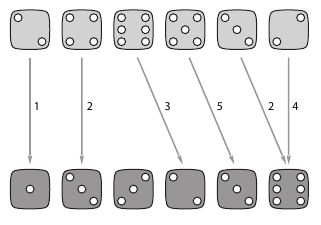
\includegraphics[scale=1]{pics/kubiki}
\caption{Две линии из шести игральных кубиков, с соответственными частичными суммами.}
\label{pic:kubiki}
\end{figure}

По построению, разница $\alpha_m-\beta_{m'}\ge 0$ не превышает $n-1$ 
(если $\alpha_m-\beta_{m'}\ge n$, то индекс $m'$ не максимален).
Если какая-то из разниц $\alpha_m-\beta_{m'}$ равна $0$, то задача решена --- в этом случае, взяв $j=s=1$, $k=m$ и $t=m'$, получим два начальных сегмента с одинаковыми суммами.
Если же ни одна из разниц $\alpha_m-\beta_{m'}$ не равна $0$, то все $n$ разниц 
$\alpha_m-\beta_{m'}$ лежат в множестве $\{1,\dots,n-1\}$ и, значит, две из них равны.
Предположим, что это $\alpha_p-\beta_{p'}$ и $\alpha_q-\beta_{q'}$.
Но тогда 
\[\sum_{i=p+1}^qa_i=\sum_{i=p'+1}^{q'}b_i.\]
--- снова победа.

Ну ведь хитр\'{о}! --- возражения не принимаются.

На рисунке есть только одна пара совпадающих разностей (обе равны 2), а именно $p=2$, $q=5$, $p'=2$ и $q'=6$;
вот соответственные подстроки с равными суммами:
\[a_3+a_4+a_5=6+5+3=3+2+3+6=b_3+b_4+b_5+b_6.\]

\begin{addedbytheeditors}
У этой идеи есть и другие применения; иногда неожиданные как например следующий результат \cite{petrunin}:
\textit{Если $\tilde M\to M$ --- $n$-листное локально-изометрическое накрытие компактного риманова многообразия $M$, то $\mathrm{diam}\, \tilde M\le n\cdot \mathrm{diam}\, M$}, где $\mathrm{diam}\, M$ обозначает \textit{диаметр $M$}, то есть максимальное расстояние между парой точек в $M$.

\textbf{Редакторам:} Надо исправить картинку --- третья стрелка слева должна указывать на 5-ку. 
\end{addedbytheeditors}

\chapter{Приключения муравья Элиса}

% читает Кноп

\setlength{\epigraphwidth}{.67\textwidth}
\epigraph{Пойди к муравью, ленивец, посмотри на действия его и будь мудрым.
}{--- Книга Притчей Соломоновых 6:6-8} 

Муравьи, даже в одномерном мире, привлекают математиков и любителей головоломок.
Я приведу десяток головоломок (все авторские, если не сказано обратное) про моего любимого муравья Элиса
(см. рис. \ref{pic:alice1}).
Каждая головоломка иллюстрирует какую-то математическую идею.

\begin{figure}[ht!]
\centering
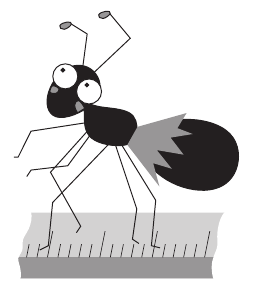
\includegraphics[scale=.7]{pics/alice1}
\caption{Муравей Элис, собственной персоной.}
\label{pic:alice1}
\end{figure}

Начнём с классической муравьиной головоломки.

\subsection*{Уже упал?}\rindex{Уже упал?}\label{Уже упал?}

На метровом стержне случайным образом расставлены 25 муравьёв; Элис стоит тринадцатым с западного конца.
Каждый муравей повёрнут на восток или на запад с равной вероятностью.
Муравьи начинают маршировать (туда, куда смотрят) со скоростью 1 см/с;
при встрече, они меняют направление движения.
Сколько надо подождать, дабы точно знать, что Элис уже упал?

\subsection*{Элис на окружности}\rindex{Элис на окружности}\label{Элис на окружности}

Теперь Элис --- один из 24 муравьёв, случайно расставленных на окружности метровой длины.
Каждый муравей случайно повёрнут по или против часовой стрелки и движется со скоростью 1 см/с.
Как и раньше, при встрече муравьи разворачиваются.
Какова вероятность того, что через 100 секунд Элис окажется точно в том же месте, где начал?

\subsection*{Какой конец?}\rindex{Какой конец?}

Муравьи опять на стержне.
Какова вероятность того, что Элис упадёт с того конца, на который смотрел вначале?

\subsection*{Кто последний?}\rindex{Кто последний?}

А какова вероятность того, что Элис упадёт последним?

\subsection*{Число столкновений}\rindex{Число столкновений}

Во время всего процесса, каково ожидаемое (то есть среднее) число столкновений муравьёв?

\subsection*{Ущерб для Элиса}\rindex{Ущерб для Элиса}

Каково ожидаемое число столкновений у самого Элиса?

\subsection*{Страховой рейтинг Элиса}\rindex{Страховой рейтинг Элиса}

Какова вероятность того, что у Элиса больше столкновений, чем у любого другого муравья?

\subsection*{Насморк}\rindex{Насморк}

Элис подхватил насморк, который мгновенно передаётся от муравья к муравью при столкновении. Сколько муравьёв заразится в среднем, прежде чем все упадут?

\subsection*{Элис посередине}\rindex{Элис посередине}

Теперь новый эксперимент.
Элис стоит точно посередине метрового стержня; 12 муравьёв расставлены случайным образом к западу от него, и ещё 12 к востоку.
Как и раньше, каждый муравей случайно повёрнут на восток или на запад и движется туда, куда смотрит, со скоростью 1 см/с, меняя направление при встрече лоб в лоб.
Однако на этот раз муравьи не падают ---
на концах стержня они разворачиваются и идут назад.
Через 100 секунд муравьи застыли на месте.
На каком максимальном расстоянии от своего начального положения Элис может оказаться?

\subsection*{Новое место Элиса}\rindex{Новое место Элиса}

На стержне теперь только 24 муравья:
12 на западной половине смотрят на восток,
остальные на восточной половине стержня смотрят на запад.
Элис --- пятый с западного конца.
Муравьи движутся как обычно, разворачиваясь при столкновениях и падая с концов.
Что требуется знать об их начальной конфигурации, чтобы сказать, где очутится Элис через 63 секунды?

\section*{Источники и решения}

\subsubsection*{Уже упал?}

Насколько мне известно, первая публикация этой замечательной головоломки состоялась в веб-колонке «Math Fun Facts» Фрэнсиса Су из Колледжа Харви Мадда \cite{math-fun-facts};
Фрэнсис припоминает, что услышал её в Европе от некого Феликса Варди, кого он не смог найти.
После этого головоломка появилась в журнале Emissary \cite[Весна/Осень 2003]{berlekamp-buhle}.

Дэн Амир, бывший ректор Тель-Авивского университета, увидел головоломку в Emissary и показал её тель-авивскому математику Ноге Алону, который принёс головоломку в принстонский Институт перспективных исследований;
я же услышал её от Ави Вигдерсона из этого института в конце 2003 года.

Ключ к этой и последующим головоломкам в том, что если бы муравьи были взаимозаменяемы, то было бы без разницы, проходят они сквозь друг друга или разворачиваются при встрече.
Тогда каждый муравей просто идёт прямо и должен упасть в течение 100 секунд.
Поскольку через 100 секунд все муравьи упали, то упал и Элис.

Если хочется избежать анонимности муравьёв, то можно думать, что каждый из них несёт флажок.
При встрече они обмениваются флажками и разворачиваются.
Таким образом, каждый муравей всегда несёт один флажок, а при встрече муравьёв флажки проходят мимо друг друга.
Если со стержня упали все флажки, то упали и муравьи.

Если начать с муравья, стоящего лицом на восток на западном конце шеста, то легко добиться того, чтоб к 100-й секунде Элис поднёс его флажок к восточному концу.
Поэтому 100 секунд ожидания необходимы и достаточны.

\subsubsection*{Элис на окружности}

Как и раньше, будем думать, что муравьи несут по флажку и обмениваются ими при встрече.
Тогда каждый флажок проходит полный круг за заданный период времени, заканчивая там, где начал.
При этом циклический порядок муравьёв не меняется, и значит (в большинстве случаев) произошёл циклический сдвиг.
То есть каждый муравей сдвинулся на определённое число позиций, скажем $k$, по часовой стрелке.
В частности, если Элис вернулся на своё место, то вернулись и все остальные.

Заметим, что если изначально $m$ муравьёв направлены по часовой стрелке, то в любой момент времени ровно $m$ муравьёв идут по часовой стрелке, и ровно $24 - m$ против.
Ведь при каждом столкновении муравей, движущийся по часовой стрелке, становится движущимся против часовой стрелки, и наоборот.
(Про это можно думать как о сохранении момента импульса!)
В любом случае, за время всего эксперимента один муравей сдвинется в среднем на $100(2m - 24)/24$ см по часовой стрелке.
Значит, каждый вернётся на своё место тогда и только тогда, когда $2m - 24$ кратно $24$; то есть, если $m = 0$, $24$ или $12$.

Первые два случая (когда все смотрят в одном направлении) имеют незначительную вероятность, но вклад последнего составляют внушительные $16{,}1180258\%$. %??? было неправильно 16,1180377 

Чтобы быть совсем точными, у нас есть $2^{24}=16\,777\,216$ вариантов выбрать направления, из которых  $\binom{24}0+\binom{24}{12}+\binom{24}{24}=1+2\,704\,156+1$ возвращают Элисa на место.
Это даёт вероятность $2\,704\,158/16\,777\,216 \z\sim 0{,}161180377$.

\subsubsection*{Какой конец?}

Заметим, что с восточного конца падают столько же муравьёв, сколько их смотрело на восток вначале.
Действительно, число муравьёв, смотрящих на восток, меняется только при падении муравья с воточного конца.
(Также можно думать об упавших со стержня флажках).
В любом случае, если $k$ муравьёв падают с восточного конца, то это происходит с $k$ самыми восточными муравьями, ведь их порядок на стержне не меняется.

Воспользовавшись симметрией, можно предположить, что вначале Элис смотрит на восток.
Как мы уже знаем, он упадёт с восточного конца, если вначале на восток смотрело $13$ или более муравьёв.
Это означает, что $12$ или более из оставшихся $24$-х смотрят на восток.
Вероятность того, что $13$ или более из $24$-х муравьёв смотрят на восток, такая же, как вероятность того, что $11$ или менее смотрят на восток, поэтому вероятность события, которое нас интересует, равна половинке плюс половине вероятности того, что ровно $12$ из $24$-х муравьёв смотрят на восток.

Последняя составляет $\binom{24}{12}/2^{24}$, что даёт $0{,}161180258$.
Получаем ответ $0{,}580590129\dots$, то есть чуть больше чем 58\%.

\subsubsection*{Кто последний?}

Можно предположить (снова используя симметрию), что Элис падает с восточного конца,
а значит и $12$ муравьёв к востоку от него делают то же самое.
Если он падает последним, то 12 муравьёв к западу от Элис упадут с западного конца.
То есть изначально ровно 12 флажков, а значит, и 12 муравьёв, повёрнуты на запад.
Это происходит с вероятностью $\binom{25}{12}/2^{24}$, то есть примерно в $31\%$ случаев.

Однако и в этом случае Элис не обязательно упадёт последним;
примерно в половине случаев эта честь достанется его западному соседу.
Таким образом, интересующая нас вероятность будет около $15{,}5\%$.

Но не стоит довольствоваться приближением, когда можно найти точный ответ.
Время, которое каждый флажок обречён провести на стержне, независимо и равномерно распределено между $0$ и $100$ секундами.
Таким образом, вероятность того, что самый долгоживущий флажок это один из 13 восточно-направленных флажков, составляет $13/25$.
Значит точный ответ $13/25 \z\times\binom{25}{12}/2^{24}$, и это уже знакомое нам число $\binom{24}{12}/2^{24}\sim 0{,}161180258$.

\subsubsection*{Число столкновений}

Каждый флажок встретится с каждым флажком расположенным впереди него и направленным к нему.
В среднем перед флажком стоит $12$ других и
половина из них (в среднем) направлена к нему.
Таким образом, флажок сталкивается с шестью другими, и всего $25 \times 6 = 150$ столкновений для всех флажков в среднем.
При этом каждое столкновение считается дважды, и ответ $75$.

А вот другой, немного более строгий способ вычисления:
Какова вероятность того, что два флажка столкнутся?
Независимо от их местоположения это происходит, только если они направлены друг к другу,
таким образом, вероятность $\tfrac14$.
По линейности матожидания число столкновений равно $\binom{25}2 \times \tfrac14 = 25 \times 24 /8 = 75$.

Кстати, максимальное число столкновений достигается, если все муравьи направлены к Элис (центральностоящему муравью).
В этом случае все $13$ флажков за Элисом сталкиваются со всеми $12$-ю флажками перед Элисом --- всего $12 \times 13 = 156$ столкновений.

Наименьшее возможное число столкновений, конечно, равно нулю, но это происходит с ничтожной вероятностью $26/2^{25} \sim 0{,}000000774860382$.


\subsubsection*{Помятость Элиса}

Легко подсчитать столкновения флажка Элиса.
Пусть Элис изначально смотрит на восток, в среднем $6$ из $12$ флажков перед Элисом, смотрят на запад.
Следовательно, в среднем  флажок Элиса столкнётся с шестью другими.

Но Элис не всегда несёт свой исходный флажок, и похоже, он сталкивается чаще других.
Почему?
Ну в среднем у муравья по шесть столкновений ($75 \z\times 2/25$), у крайних не больше одного, а у Элиса, стоящего посредине, должен быть больше среднего.

Заметим, что каждый муравей сталкивается только со своими двумя соседями,
и чередует их (ведь и его направление чередуется между столкновениями).
Последнее столкновение муравья будет с его западным соседом, если он свалится с восточного конца, и наоборот --- с его восточным соседом, если он свалится с западного конца.

Предположим, что вначале $k$ муравьёв смотрят на запад.
Поскольку их флажки идут к западному концу, $k$ самых западных муравьёв сваливаются с западного конца.
Тот из них, кто вначале смотрел на запад, имеет одинаковое число столкновений с обоих сторон;
тот же, кто смотрел на восток, имеет на одно столкновение больше с восточной стороны.
Таким образом, число столкновений между $j$-ым  (считая с запада) и 
$(j+1)$-ым муравьём равно числу, смотрящих на восток, среди муравьёв от $1$ до $j$ --- при условии, что $j\le k$.

В силу симметрии можно предположить, что $k$ находится между $13$ и $25$ (так, что Элис сваливается с западного конца).
Тогда число столкновений между Элис и его западным соседом равно числу муравьёв, смотрящих на восток, к западу от Элис; обозначим это число $x$.
Значит общее число столкновений Элиса будет равно $2x$ или $2x+1$ в зависимости от того, смотрел он на запад или восток вначале.

Априорное матожидание $\mathbb{E}[x]$ для $x$ равно $6$, так как западнее Элис $12$ муравьёв, каждый из которых может смотреть в любом направлении.
Однако мы только что предположили (чёрт!), что больше половины муравьёв смотрят на запад.
Но обратите внимание, что поскольку ожидаемое число муравьёв, смотрящих на восток, к востоку от Элис также равно $\mathbb{E}[x]$, число, которое мы ищем, является именно общим ожидаемым числом муравьёв, смотрящих на восток, даже учитывая, что они в меньшинстве.

Предположим, что муравьи были расставлены в алфавитном порядке, и последним стоял Яша.
Существует $2^{25}/2=2^{24}$ способа сделать такое распределение, чтобы получить большинство западных направлений и $\binom{24}{12}$
из них дают ровно $12$ муравьёв, направленных на восток, среди первых $24$ муравьёв.
В этом случае Яша обязан смотреть на запад,
а в остальных случаях он равновероятно смотрит на запад или на восток.
Следовательно, вероятность того, что Яша смотрит на восток, составляет
$0{,}419409871$.

Поскольку вероятность того, что Яша смотрит на восток, не отличается от этой же вероятности для любого другого муравья, умножив её на $25$, получим матожидание числа муравьёв, смотрящих на восток, что примерно $10{,}4852468$.
Именно это и является средним числом столкновений Элиса.

\subsubsection*{Страховой рейтинг Элиса}

Предположим, что самые западные $k$ муравьёв падают с западного конца,
а остальные с восточного.
Мы уже видели в предыдущем решении, что если $c_i$ --- число столкновений между $i$-ым (считая с западного конца) и $(i + 1)$-ым муравьём, то $c_i$ остаётся тем же или увеличивается на $1$ до $i = k$; после этого остаётся тем же или уменьшается на $1$.
В частности, $c_i=c_{i-1}$ ровно тогда, когда $i$-ый муравей смотрит (изначально) в том же направлении, с которого он упадёт.

Число столкновений $i$-го муравья равно $c_{i-1}+c_{i}$.
Значит, Элис обойдёт всех по числу столкновений, если $c_{11}+c_{12}\z<c_{12}\z+c_{13}\z>c_{13}\z+c_{14}$, а это значает, что  $c_{11}<c_{13}$ и $c_{12}>c_{14}$.
Это может произойти только если $c_{11}<c_{12}=c_{13}>c_{14}$, а значит, что $k = 12$ или $13$, и что Элис смотрит в том направлении, с которого падает,
и что оба его соседа смотрят в противоположные стороны от тех концов, с которых они падают.
Похоже, что это даёт вероятность 
\[\left(\tbinom{25}{12}+\tbinom{25}{12}\right)/2^{25}\cdot (\tfrac12)^3\sim 3.87452543\%,\]
однако эти события не совсем независимы.

Предположим, что Элис смотрит на восток, его восточный сосед --- Шурик, а западный сосед --- Юрик.
Шурик, как и Элис, будет падать с восточного конца и, следовательно, изначально должен был смотреть на запад (вероятность $1/2$).
Юрик --- один из $12$ муравьёв, падающих с западного конца и, следовательно, вначале он смотрел на восток (опять вероятность $1/2$).
Из оставшиеся 22 муравьёв половина должна смотреть на запад, а половина на восток (вероятность $\binom{22}{11}/2^{22}$), поэтому точный ответ составит
\[\left(\frac12\right)^2\cdot\binom{22}{11}/2^{22}\sim 4{,}20470238\%.\]

\subsubsection*{Насморк}

Эта головоломка чисто комбинаторная, как и многие другие в этой главе.
В частности, хоть это и не совсем очевидно, ответ не зависит от длины стержня.
Может показаться, что более короткий стержень позволит некоторым муравьям выбраться с него до того, как они успеют заразиться, однако как только муравей направляется к концу и перед ним нет других, его столкновениям пришёл конец.

Наверно, проще всего считать, что заражаются не муравьи, а флажки.
Мы можем предположить, что Элис смотрит на восток.
Тогда флажки, направленные на запад впереди него, встретят его флажок и заразятся.
В то же время флажки, направленные на восток впереди него, избегут заражения.
Тем временем флажки, направленные на запад, после встречи с флажком Элиса, заражают все флажки, направленные на восток позади Элиса, и в то же время флажки, направленные на запад позади Элис, избегут заражения.

Поскольку в среднем впереди Элиса находится 6 флажков, направленных на запад, и 6 флажков, направленных на восток, у нас 13 заражённых флажков (включая флажок Элиса) и, таким образом, всего 13 заражённых муравьёв в среднем.

Однако в наше рассуждение закралась небольшая ошибка: если впереди Элиса вовсе нет муравьёв, смотрящих на запад, то нет и флажка, который мог бы встретить флажок Элиса и заразить флажки, направленные на восток, позади него.
Такое происходит с вероятностью $1/2^{12}$ и уменьшает ожидаемое число заражённых с $7$ (Элис плюс в среднем 6 флажков, направленных на восток, позади него) до 1 (только Элис).
Таким образом, правильный ответ не $13$, а $13 - 6/2^{12} \sim 12{,}9985352$ заражённых муравьёв в среднем.

\subsubsection*{Элис посредине}

Джон Гилфорд из Agilent Technologies показал эту головоломку Стэну Вагону,
тот однажды осенью 2003 года объявил её «задачей недели» колледжа Макалестер.
Я узнал о задаче в январе 2004 года от Элвина Берлекэмпа на конференции «Joint Mathematics Meetings» в Финиксе.
Именно тогда главный герой этой главы получил своё имя;
думаю, что у Элвина действительно есть тётя Элис.
На меня ещё повлияло и присутствие на конференции издателя этой книги, Элис Питерс из A K Peters, Ltd.

Предположим, как обычно, что каждый муравей несёт флажок, и флажками обменивается при встрече.
Затем каждый флажок проходит ровно один метр, один раз отскакивая от конца и заканчивая свой путь в точке, симметричной его начальной позиции.
В частности, флажок Элис заканчивает свой путь снова в центре. Но будет ли Элис его нести?

Несоменно будет, потому что муравьи остались в исходном порядке.
$12$ флажков с западной стороны теперь находятся на восточной, и наоборот, так что у Элиса опять $13$-й флажок, и сам Элис всё ещё $13$-й с конца.

Таким образом, Элис оказывается там, где начал.
Другими словами, максимальное расстояние, на которое он может отойти от своей начальной точки, равно нулю.

\subsubsection*{Новое место Элиса}

Это вариация головоломки, придуманной Ногой Алоном и Одедом Маргалитом из Тель-Авивского университета, которую передал мне Нога.

Пусть $x_1,\dots,x_{12}$ --- начальные позиции $12$ муравьёв, обращённых на запад, пронумерованные с запада на восток.
Позиции задаются в сантиметрах от западного конца.
Положим, что $k$ таково, что флажки, стартовавшие с $x_k,\dots,x_{12}$, не упадут, и следовательно окажутся в позициях $x_k-63,\dots,x_{12}-63$.

Муравьи, конечно же, не меняют порядка на стержне.
Поскольку $k-1$ флажок упадёт с западного конца, Элис упадёт в случае если $k> 5$.
В противном случае он становится $(6-k)$-м оставшимся муравьём, считая с западного конца, что помещает его в позицию $x_{k+(5-k)}-63=x_5-63$.
Таким образом, всё, что вам нужно знать, это позиция 12-го муравья к востоку от Элиса, то есть $17$-го от западного конца.
Элис окажется на $63$ см к западу от этой точки;
если эта точка уже находится менее чем в $63$ см от западного конца, то Элис свалился.

\begin{figure}[ht!]
\centering
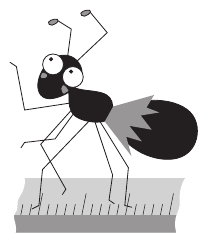
\includegraphics[scale=1]{pics/alice2}
\caption{Элис прощается.}
\label{pic:alice2}
\end{figure}

\chapter{Многословное отступление: Игра ХОМО}

%You could leave it out, or keep it in English, but the best option would be to redo the game in Russian!
%To do that, I'd suggest getting a good computer wordlist (e.g., a list of Scrabble-eligible Russian words), and write a program that checks for rare substrings.
%Then pick out the ones that are particularly clever or amusing, and you'll have a great list of Russian HIPEs. 

%Of course it is possible that, since spelling in Russian is more reliable than in English, the game of HIPE doesn't work as well in Russian.
%But why not give it a try?

%---Pete

Рассматривайте эту главу как антракт, --- перерыв, не связанный с математикой. Однако многие математики любят игры со словами, и (по моему личному опыту) эту в особенности. 

Возможно, вы слышали такую загадку: какое английское слово содержит четыре последовательных буквы, которые являются последовательными буквами алфавита?
Ответ: undeRSTUdy.
Вдохновившись этой и другими словесными головоломками, я и ещё трое старшеклассников на летней программе Национального научного фонда в 1963 году начали обстреливать друг друга комбинациями букв, требуя найти слово, содержащее эту комбинацию\footnote{Здесь и далее автор, разумеется, «обстреливает» читателя английскими примерами. Мы постарались, сохранив дух главы, насытить её аналогичными русскими примерами, и даже название игре дали своё собственное. \pr}.

Между буквами, входящими в комбинацию, не должно быть других букв.
Пример:
\textbf{ТСЧ} = оТСЧёт,
\textbf{МПЦ} = презуМПЦия.
В некоторых загаданных комбинациях были всего две буквы, например, 
\textbf{ЦД} = плаЦДарм, 
\textbf{ГШ} = флаГШток (или другое заимствованное из немецкого языка слово, зинГШпиль).
Начните с \textbf{ОДС} (подсказка: здесь более одного возможного ответа, но один лежит совсем на поверхности). 

Удвоенные буквы 
(\textbf{ЧЧ}, \textbf{ГГ} и даже \textbf{АА}) могут быть интересными, но самые сложные загадки, которые мы отыскали, --- это комбинации из трёх или четырёх букв.
Мы назвали игру в честь комбинации \textbf{ХОМО} = муХОМОр%
\footnote{В оригинале у П. Уинклера было название \textbf{HIPE} от arcHIPElago.}.
Конечно, ХОМО, несомненно, изобретали и переизобретали тысячи раз, и вы не обязаны использовать наше название --- но всё равно полезно как-то её назвать. 

При придумывании заданий в ХОМО есть очень естественная цель --- искусно замаскировать отгадку;
ещё приятнее, если отгадка окажется распространённым словом, которое тем не менее тяжело найти. 

Например, у \textbf{ОТОЙ} решается одним из самых распространённых слов, но сможете ли вы его найти?
Ведь забавно поставить приятеля в тупик, задав ему, например \textbf{СОБЬ}, а потом ещё сказать, что нужно добавить всего одну букву! 

В идеале лучше, чтоб решение было единственным (среди нарицательных существительных, имена собственные в этой игре не используются), но это не является строго обязательным требованием, если вы играете с друзьями.

ХОМО-загадки из более чем четырёх букв редко бывают интересными, потому что много известных букв подряд даёт уж очень много информации.
Так что мы ограничились буквосочетаниями из двух, трёх и четырёх букв.
Хотя, например, \textbf{УКВОС} тоже вполне неплохая загадка, не так ли?

В общем, попробуйте свои силы.

Загадки из двух букв:

\begin{multicols}{4}
{\bf
ГБ

ГЗ

ГШ

ЖЧ

ЖЮ

ЗФ

ЙГ

ЙЯ

КП

КФ

ЛФ

МД

МТ

ПД

СЖ

ТЖ

ФЧ

ХХ

ХЪ

ЦН

ЧЧ

ШЦ

ЩМ

ЫИ

ЬЭ

ЮИ
}
\end{multicols}

Ответы:

\begin{multicols}{2}

реГБи

шлаГБаум

зиГЗаг

флаГШток

зинГШпиль

муЖЧина

ЖЮри 

фиЗФак

таЙГа 

саЙГак

маЙЯ 

папаЙЯ

секвоЙЯ

параноЙЯ

аллилуЙЯ

блоКПост

роКФор

саЛФетка

шаЛФей

фиЛФак

аЛФавит

заМДекана

лоМТик

драМТеатр

экспроМТ

проМТовары

креПДешин

СЖигание

СЖатие

СЖимаемость

оТЖим

оТЖиг

борТЖурнал

шкаФЧик

треХХвостка

сверХЪестественность

спеЦНаз

каприЧЧио

мыШЦа

веЩМешок

вЫИгрыш

белЬЭтаж

сЮИта 

флЮИд

трЮИзм
\end{multicols}

Загадки из трёх букв:
\begin{multicols}{4}
{\bf
БСЦ

ДДВ

ДМН

ДСН

ДЧУ

ИЭД

ЛГЕ

МБД

МРУ

НКН

НТВ

НУУ

ОЯБ

ПФР

РАЭ

РГК

РГС

РКК

РРУ

РХЗ

САЭ

ТАЭ

ТИЭ

ТСР

ТСЧ

ТФИ

УСФ

УЧЛ

ФМЕ

ФМИ

ХГР

ХУГ

ХЧЛ

ЦШК

ЯТЫ
}
\end{multicols}

Ответы:


\begin{multicols}{2}

аБСЦисса

преДДВерие

поДМНожество

поДСНежник

преДЧУвствие

полИЭДр

аЛГЕбра

ляМБДа

изуМРУд

баНКНота

глиНТВейн

контиНУУм

нОЯБрь

грейПФРут

тетРАЭдр

оРГКомитет

оРГСтекло

аРККосеканс

аРККотангенс

аРККосинус

коРРУпция

свеРХЗадача

гекСАЭдр

икоСАЭдр

окТАЭдр

пенТАЭдр

гепТАЭдр

пяТИЭтажка

отсрочка

оТСЧёт

мульТФИльм

полУСФера

двУЧЛен

ариФМЕтика

логариФМИрование

треХГРанник

четыреХГРанник

четыреХУГольник

треХЧЛен

спеЦШКола

свЯТЫня
\end{multicols}

Загадки из четырёх букв
\begin{multicols}{4}
{\bf
АТЫН

АЧЕЛ

ВАБР

ГОУГ

ГРИР

ДМНО

ЕПИП

ЗОЦИ

ИМАД

ИФМИ

ИЩЕТ

КАЧО

ЛЕЛЕ

ЛУОК

МАША

НАЧО

НЕРЛ

НСОИ

РКТА

СС-Р

УШЛА

ФМОМ

ФУРК

ХУГО

ЯГИН
}
\end{multicols}

Ответы:

\begin{multicols}{2}
лАТЫНь

кАЧЕЛи

шВАБРа

мноГОУГольник

интеГРИРование

поДМНОжество

параллелЕПИПед

бенЗОЦИстерна

прИМАДонна

логарИФМИрование

нИЩЕТа

сКАЧОк

паралЛЕЛЕпипед

поЛУОКружность

маМАША

зНАЧОк

пиоНЕРЛагерь

тангеНСОИда

аРКТАнгенс

преСС-Релиз

бУШЛАт

ариФМОМетр

биФУРКация

четыреХУГОльник

кнЯГИНя
\end{multicols}

\chapter{2D и 3D}

\setlength{\epigraphwidth}{.83\textwidth}
\epigraph{Математики давно считают унизительным заниматься задачами элементарной геометрией в размерностях два и три, несмотря на то что как раз такая математика имеет практическую ценность.}{Бранко Грюнбаум и Джеффри Шепард,\\ Handbook of Applicable Mathematics}

Для многих первое знакомство с теоремами и доказательствами
происходит при изучении евклидовой плоскости
в старших классах школы.
Однако сейчас вам придётся решать задачи далеки от «Начал» Евклида;
они проверят насколько глубоко вы проникли в мир двух и трёх измерений.

\subsection*{Монеты на столе}

На прямоугольном столе лежат 100 идентичных монет так, что нельзя добавить ещё монету без налегания.
(Монета может выступать за край, главное, чтобы её центр находился на столе.)
Докажите, 400-та таких монет достаточно чтобы покрыть весь стол!
(Монеты могут пересекаться и выступать за край стола).

\parit{Примечание:}
Предполагается, что каждая монета является идеальным кругом пренебрежимо малой толщины.

\subsection*{Четыре точки с двумя расстояниями}

Опишите все расположения четырёх точек на плоскости таких, что меду их парами есть только два различных расстояния.

\subsection*{Преступница и собака}

Преступница содержится в поле, окружённом круглым забором.
Её охраняет свирепая собака, она способна бегать вчетверо быстрее преступницы, но приучена бегать только вдоль забора.
Если преступница подбежит к забору в месте, где собаки нет, то сможет мгновенно его перелезть и сбежать.
Но сможет ли она добраться до какой-то точки забора быстрее собаки?

\subsection*{Теннисная загадка}

Мяч при подаче попал \emph{вне поля}, но ни один из линейных судей не может сказать «аут».
Где же он приземлился?

\parit{Замечание:}
На крупном теннисном турнире каждый линейный судья отвечает за одну линию и объявляет «аут», когда мяч пролетает мимо этой линии и приземляется на неправильной стороне.
К сожалению, возможен удар вне поля, который к этому не приводит; что это за удар?

\subsection*{Двойное покрытие прямыми}

Используя два полных набора параллельных прямых, можно покрыть плоскость так, что каждая точка лежит ровно на двух прямых.
Можно ли сделать это иным способом, то есть покрыть каждую точку плоскости ровно дважды, используя набор прямых, с более чем двумя разными направлениями?

\parit{Замечание:} К примеру, можно попробовать взять все прямые, касающиеся некоторой окружности.
Это отлично работает за пределами окружности, но точки на окружности покрыты лишь раз, а те, что внутри вовсе не покрыты.

\medskip

Подошло время для трёхмерных задач.

\subsection*{Кривая на сфере}

Докажите, что если замкнутая кривая на единичной сфере короче $2\pi$, то она содержится в какой-то полусфере.

\parit{Замечание:} Похоже на правду, ведь периметр большого круга (границы полусферы) равен $2\pi$.
Но как это доказать?

\subsection*{Лазерная пушка}

Вы стоите в большой прямоугольной комнате с зеркальными стенами.
В другом месте этой комнаты стоит ваш враг с лазерной пушкой.
Вы оба --- идеальные точки.
Единственный способ защититься от лазера --- расставить телохранителей (тоже точки) в комнате так, чтобы они поглощали лазерный лучи.
Сколько телохранителей необходимо для защиты от всех возможных выстрелов?

\parit{Замечание:} «Бесконечно много» --- приемлемый ответ, если конечно он верен!

\medskip

Мы завершаем главу замечательной задачей, применимой в обычной жизни.
Часто для определения стоимости отправки или доставки прямоугольного ящика складывают его длину, ширину и высоту,
и находят эту сумму в таблице;
конечно же, чем больше сумма, тем выше стоимость.
Можно ли сэкономить на стоимости отправки, засунув какой-то ящик в ящик побольше, но подешевле?

\subsection*{Ящик в ящике}

Допустим, что стоимость прямоугольного ящика равна сумме его длины, ширины и высоты.
Докажите или опровергните: невозможно уместить ящик в более дешёвый ящик.

\parit{Замечание:}
Очевидно, что длинный тонкий ящик можно поместить в более короткий, расположив его вдоль диагонали;
но, похоже придётся слишком много пожертвовать другими двумя измерениям.
На плоскости, то есть с прямоугольниками, используя неравенство треугольника, легко увидеть, что аналогичная экономия невозможна.
Но вроде бы, этот метод не работает в трёхмерном пространстве.

\section*{Источники и решения}

\subsubsection*{Монеты на столе}

Эта интересная головоломка досталась мне от специалиста по информатике Гая Киндлера во время чудесного года, проведённого нами в принстонском Институте перспективных исследований.

\begin{figure}[t!]
\centering
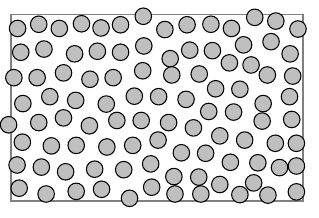
\includegraphics[scale=1]{pics/coin1}
\caption{Нельзя добавить новую монету без перекрытия со старыми.}
\label{pic:coin1}
\end{figure}

\begin{figure}[b!]
\centering
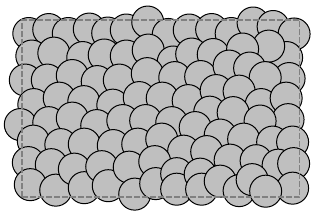
\includegraphics[scale=1]{pics/coin2}
\caption{Стол покрыт удвоенными монетами.}
\label{pic:coin2}
\end{figure}

Начнём с того, что если удвоить радиус каждой монеты (скажем, с $1$ до $2$), то как видно на рисунках \ref{pic:coin1} и \ref{pic:coin2}, покроется весь стол.
Почему?
Ну если какая-то точка $P$ не покрыта, то она лежит на расстоянии $2$ или более от центра любой монеты, так что к исходной конфигурации можно было добавить (маленькую) монету, с центром в $P$.

Дело было бы сделано, если бы большая монета покрывалась четырьмя маленькими.
Однако это не так.

Тем не менее нужным свойством обладает \emph{сам} прямоугольник --- он разбивается на четыре уменьшенные копии самого себя.
Итак, сожмём вдвое всю картинку (рис. \ref{pic:coin2}, где большие монеты покрывают весь стол) и воспользуемся четырьмя её копиями (как на рис. \ref{pic:coin3}).
Так мы покроем весь исходный стол!


\begin{figure}[t!]
\centering
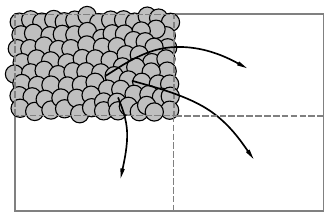
\includegraphics[scale=1]{pics/coin3}
\caption{Четыре уменьшенные стола покрывают стол целиком.}
\label{pic:coin3}
\end{figure}

\medskip

Это красивое рассуждение, выглядит грубым, однако (как ни странно) оно даёт наилучшую оценку --- замените $4$ на что-то меньшее, скажем, $3{,}99$, и полученное утверждение перестанет быть верным.

Чтобы это понять, рассмотрим предельный случай, когда стол очень большой, а монет так много, что граничные эффекты пренебрежимо малы.
Заменим стол на пол ванной комнаты, покрытый мозаикой в виде пчелиных сот;
то есть каждая плитка это правильный шестиугольник диаметра (скажем) 2.
Сама плитка имеет площадь $6\times\sqrt{3}/4=3\times\sqrt{3}/2$, ведь каждая плитка разбивается на шесть равносторонних треугольников со стороной 1 и, значит, площади $\sqrt{3}/4$.

\begin{figure}[t!]
\centering
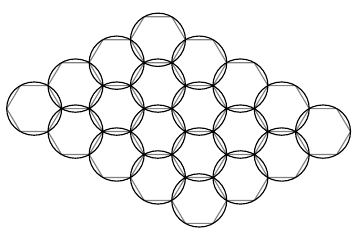
\includegraphics[scale=1]{pics/coin4}
\caption{Покрытие описанными кругами правильных шестиугольников.}
\label{pic:coin4}
\end{figure}

\begin{figure}[b!]
\centering
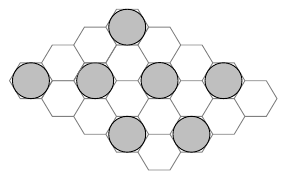
\includegraphics[scale=1]{pics/coin5}
\caption{Разряженная конфигурация.}
\label{pic:coin5}
\end{figure}

Весь пол можно покрыть, положив на каждую плитку монету, граничная окружность которой описана вокруг плитки (см. рис. \ref{pic:coin4}).

Тогда каждая монета имеет радиус $1$ и, следовательно, площадь~$\pi$.
Если $A$ --- площадь всего пола, то, игнорируя граничные эффекты, общая площадь монет будет $\pi A/(3\sqrt{3}/2)\sim 1{,}2092\times A$.

Теперь разберёмся, насколько разрежённо можно расположить монеты на полу, чтобы нельзя было добавить новую монету без перекрытия со старыми.
Воспользуемся той же плиткой, но на этот раз покроем только треть плиток (рис. \ref{pic:coin5}).
В середину каждой такой плитки положим по монете с радиусом чуть больше радиуса вписанной в шестиугольник окружности. 
Это не позволит добавлять монет.

Какова же площадь всех этих монет?

Радиус монеты чуть больше высоты одного из шести равносторонних треугольников, составляющих шестиугольник — а именно, $\sqrt{3}/2$.
Следовательно, площадь монеты чуть превысит $\pi \z\times (\sqrt{3}/2)^2 \z= 3\pi/4$.

Отсюда следует, что общую площадь монет на полу можно сделать произвольно близкой к $(1/3) \times (3\pi/4) \times A/(3\sqrt{3}/2) = \pi A/(6 \sqrt{3}) \z\sim 0{,}3023 \times A$, а это ровно четверть того, что было раньше!

\medskip

Мы не только решили головоломку, но и доказали пару экстремальных свойства кругов.

Первое утверждает, что нет лучшего способа покрыть плоскость единичными кругами, чем описать круги вокруг плиток шестиугольной мозаики, как мы сделали выше.
Второе, --- что нет более разреженной конфигурации монет \emph{без} возможности добавить лишнюю, чем помещать на каждой третьей плитке круг, чуть больший, чем вписанный, опять же, как мы проделали выше.

Если вам эти свойства очевидны, то подумайте о следующем ещё более очевидном утверждении: \emph{самая плотная упаковка единичных кругов на  плоскости получается из кругов, вписанных в шестиугольники пчелиных сот}.
Это было доказано только в 1972 году видным венгерским геометром Ласло Фейешем Тотом (1915---2005)!

\begin{addedbytheeditors}
Доказательства всех трёх последних утверждений приводятся в замечательной книжке Фейеша Тота \cite[III §3]{tot}.
Конечно же все они были доказаны раньше публикации немецкого оригинала книги в 1953 году, а никак не в 1972 году!
Приведённые в решении аргументы на примере двумерного случая иллюстрируют связь между двумя фундаментальными задачами геометрии чисел~--- проблемой упаковки шаров и задачей о покрытии пространства перекрывающимися шарами. Подробности на эту тему см. в книге Джона Конвея и Нила Слоэна \cite{conway-sloane}. 

У задачи про монеты есть две вариации. Они отличаются тем, что связывают между собой упаковки (в первом случае) и покрытия (во втором) кругами разных радиусов. 
Если на прямоугольный противень помещается $100$ печений радиуса $2$, то на такой же противень поместится и $400$ печений радиуса $1$.
Если прямоугольник можно покрыть (без просветов, но разрешается вылезать за пределы) $100$ кругами радиуса $2$, то его можно покрыть и $400$-ми кругами радиуса $1$.
\pr
\end{addedbytheeditors}

\subsubsection*{Четыре точки с двумя расстояниями}

Эта замечательная головоломка годится для болтовни за обедом;
она была включена в раздел головоломок журнала «Pi Mu Epsilon» \cite[1985 год, задача 3a, предложена Ш. Дж. Эйнхорном и И. Дж. Шёнбергом]{16}.
Позже появилась на первой странице книги Ноба Ёсигахары \cite{61}, где была приписана Дику Хессу.

Я заметил, что очень мало людей находят все шесть конфигураций;
почти каждый упирается в какое-то препятствие или совершает ошибку, пропуская одну из них.
При этом непредсказуемо, \emph{какую} именно; один из испытуемых упустил квадрат!

\begin{figure}[ht!]
\centering
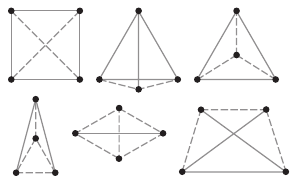
\includegraphics[scale=1]{pics/2dist}
\caption{Все шесть вариантов.}
\label{pic:2dist}
\end{figure}

Все конфигурации показаны на рис. \ref{pic:2dist}.
Последняя из них (трапеция) образована четырьмя вершинами правильного пятиугольника.


\subsubsection*{Преступница и собака}

Моё внимание к этой интересной задаче привлёк Хулио Дженовезе;
она появилась в книге Мартина Гарднера \cite{24}.

Будем считать, что круг имеет единичный радиус.
Представим, что преступница бегает в меньшем концентрическом круге радиуса $r$, где $r < \tfrac14$.
Тогда она сможет попасть в точку круга, которая находится на максимальном расстоянии от собаки (см. рис. \ref{pic:dog}).
Это потому, что длина окружности меньшего круга составляет меньше четверти длины забора.

Если $r$ достаточно близко к $\tfrac14$, то преступница может бежать прямо к забору.
Это расстояние чуть больше чем $3/4$, а собаке придётся пробежать пол окружности поля, то есть $\pi$.
Так как $\pi > 3$, это более чем в четыре раза превысит путь преступницы.

\begin{figure}[h!]
\centering
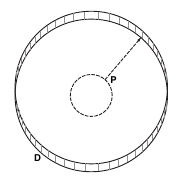
\includegraphics[scale=1]{pics/dog}
\caption{Точка, из которой преступница бежит к забору.}
\label{pic:dog}
\end{figure}

Преимущество собаки в скорости можно увеличить с $4$ до $4{,}6033388$; при этом лучшая стратегия обеих сторон приведёт к тому, что они финишируют одновременно.
Больше информации об этой задаче  можно найти на сайте головоломок IBM «Ponder This» за \cite[май 2001]{ponder-this}.

\subsubsection*{Теннисная загадка}

На этот недочёт указал мне Дик Хесс --- знаток головоломок и тенниса.
На рис. \ref{pic:tenis} показано место приземления мяча; и это ошибка при подаче --- мяч не задевает «коробку» подачи, но при этом задевает две линии линейных судей. 
Использование электронных систем контроля задней линии не помогает.
Интересно бы выяснить, часто ли такая подача ошибочно засчитывается.

\begin{figure}[ht!]
\centering
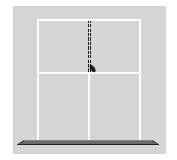
\includegraphics[scale=1]{pics/tenis}
\caption{Кто должен увидеть эту ошибку при подаче?}
\label{pic:tenis}
\end{figure}


\subsubsection*{Двойное покрытие прямыми}


Некоторых читателей это разочарует, но ответ да (если принять аксиому выбора), и есть уйма способов это сделать. 
Однако доказательство требует трансфинитной индукции (!), не оставляя места геометрии.
Задачу (и её решение) мне подбросил физик Сеня Шлосман, который не знает её происхождения.

Данное решение мне нравится как пример простого применения мощного инструмента.
Идея в следующем: мы начинаем с трёх пересекающихся прямых, так что у нас уже есть три направления.
Пусть $\kappa$ --- наименьший ординал мощности континуум (то же, что множество точек на прямой, точек на плоскости или углов на плоскости).
Посмотрим на множество ординалов ниже $\kappa$.
Каждый из них --- либо последовательный ординал (как, например, $17$, $188$ или $\omega + 1$), либо предельный ординал (как, например, $\omega$, первый бесконечный ординал); у каждого мощность строго меньше континуума.
Мощность ординалов ниже $\kappa$ --- континуум, поэтому этими ординалами можно пометить все точки плоскости.
Теперь точки плоскости образуют \emph{вполне упорядоченное} множество, то бишь каждое непустое подмножество содержит точку с минимальной меткой.

Приступим к трансфинитной индукции.
Предположим, у нас есть конфигурация прямых, покрывающая все точки множества точек $S$ с метками меньше $\sigma$ ровно дважды,
точка $P$ с меткой $\sigma$ покрыта менее двух раз,
и ни одна из точек плоскости не покрыта три раза или более.
Напомним, что $\sigma$ --- ординал, меньший $\kappa$.
Можно считать, что каждая прямая в конфигурации проходит через одну из точек множества $S$, и, значит, прямых в конфигурации меньше чем континуум.
Значит, и мощность всех двойных точек конфигурации меньше континуума.
Так как множество направлений прямых континуально, через точку $P$ можно провести прямую, не проходящую через двойные точки,
то есть её можно добавить к нашей конфигурации.
Если $P$ всё ещё не двойная, то придётся повторить ещё один раз.

Похоже на обман?
Ну да; наше построение совсем не конструктивно.
Означает ли это, что \emph{не существует} хорошего построения двойного покрытия?
Нет, но я такой пример найти не смог; не смог и Сеня.

\begin{addedbytheeditors}
Всего есть $2^{\mathfrak{c}}$ решений --- столько даёт приведённое решение, а больше быть не может, поскольку $2^{\mathfrak{c}}$ это мощность всех подмножеств прямых на плоскости.\pr
%\textbf{Редакторам:} Я переписал заново абзац с трансфинитной индукцией --- оригинал написан очень криво.
\end{addedbytheeditors}


\subsubsection*{Кривая на сфере}

Эту головоломку мне подкинул физик Сеня Шлосман, который услышал её от Алекса Красносельского.
Предложенное Сеней решение следующее.

Выберем любую точку $P$ на кривой, пройдём вдоль кривой половину её длины до точки $Q$.
Пусть $N$ будет точкой сферы на полпути между $P$ и $Q$.
(Будем думать, что $N$ это северный полюс; эта точка определена однозначно, поскольку сферическое расстояние $d(P, Q)$ от $P$ до $Q$ меньше $\pi$.)
Полюс $N$ определяет экватор, и если кривая полностью находится в северном полушарии, то дело сделано.
В противном случае кривая пересечёт экватор.
Пусть $E$ --- одна из точек пересечения.
Тогда $d(E,P) + d(E,Q) = \pi$, ведь если отразить $P$ в экваториальной плоскости, то полученная точка $P'$ будет антиподом $Q$; и, следовательно, $d(E, P') + d(E, Q) = \pi$.

Однако для любой точки $X$ на кривой сумма $d(P, X) + d(X, Q)$ меньше $\pi$, и это приводит к противоречию.

Омер Ангел из Университета Британской Колумбии
предложил другое доказательство,
менее элементарное, но все же изящное и познавательное.
Пусть $C$ --- наша замкнутая кривая, а $\hat C$ --- её выпуклая оболочка, то бишь наименьшее выпуклое множество, содержащее~$C$.
Если $C$ не содержится в полусфере, то $\hat C$ содержит начало координат;
в противном случае $0$ можно было бы отрезать от~$\hat C$ плоскостью.
Таким образом, по теореме Каратеодори (смотри ниже), существует набор из четырёх точек на $C$, выпуклая комбинация которых даёт $0$.
Другими словами, тетраэдр, вершинами которого являются эти четыре точки, содержит начало координат.

Давайте теперь двигать эти точки непрерывно друг к другу вдоль кривой.
Когда точки слились вместе, их тетраэдр уже не содержит начало координат, так что где-то по дороге начало координат оказалось на одной из граней тетраэдра.
Три точки, определяющие эту грань, лежат на большом круге, и самый короткий маршрут между любой из пар идёт по этому экватору, не проходя через оставшуюся третью точку.
Следовательно, сумма попарных расстояний трёх точек равна $2\pi$, что невозможно, так как все они лежат на $C$.

Математик Константин Каратеодори (1873---1950) доказал множество красивых теорем.
Вот одна из наиболее известных: \textit{если $v$ содержится в выпуклой оболочке некоторых точек $d$-мерного  пространства, то $v$ лежит и в выпуклой оболочке подмножества из не более чем $d+1$ из этих точек.}

Чтобы это доказать, отметим, что принадлежность точки выпуклой оболочке множества
эквивалентна тому, что точка представима как конечная линейная комбинация точек этого множества с положительными коэффициентами, сумма которых равна $1$.
Пусть $k>d+1$, и положим $v=\sum_{i=1}^k a_iv_i$, где $\sum_{i=1}^k a_i=1$ и $a_i>0$ при любом $i$.

Поскольку есть более чем $d$ векторов $v_1-v_i$ при $i=2,\dots,k$, эти векторы линейно зависимы;
следовательно, существуют коэффициенты $b_i$, не все равные нулю, такие что $\sum_{i=2}^k b_i(v_1-v_i)=0$.
Положим $b_1=-\sum_{i=2}^k b_i$; тогда $\sum_{i=1}^k b_i v_i=0$ и $\sum_{i=1}^k b_i=0$, но $b_i\ne 0$ для какого-то $i$.
Таким образом, $v=\sum_{i=1}^k a_iv_i-r\sum_{i=1}^k b_iv_i=\sum_{i=1}^k (a_i-rb_i)v_i$ для любого вещественного $r$.
В частности, если $r$~--- наименьшее отношение $a_i/b_i$  при $b_i>0$ (пусть оно достигается, скажем, при $i=j$), то $r$ положительно, и $a_i-rb_i\ge0$ для всех $i$.
Таким образом, $v$ представимо в виде выпуклой комбинации, по крайней мере, один из коэффициентов которой (а именно, $a_j-rb_j$) равен нулю, так что $v$ находится в выпуклой комбинации не более чем $k-1$ точек.
Остаётся повторять процесс, пока число $k$ не уменьшимся до $d+1$.

\begin{addedbytheeditors}
Головоломка использовалась как промежуточный результат \cite[Satz I$'$]{fenchel}
в доказательстве Вернера Фенхеля, что \emph{любая замкнутая кривая в пространстве обязана повернуть хотя бы на полный оборот}.
Его доказательство почти совпадает со вторым из приведённых выше.
(Кстати, согласно теореме Фари --- Милнора, \emph{любой узел обязан повернуть хотя бы на два полных оборота}; обзор шести различных доказательств этой теоремы представлен в \cite{petrunin-stadler}.)

Этот результат и его обобщения востребованы в дифференциальной геометрии.
По следам одной беседы за обедом 1997 года, Боб Фут собрал из различных его доказательств короткую заметку.
Первое из доказательств в его коллекции практически совпадает с первым приведённым здесь;
его нашли Майк Керкхов, Дан Клинг и сам Боб Фут.
Улучшение этого доказательства принадлежит Стефани Александер, оно, между прочим, обсуждается в ютубовском ролике Серхио Заморы \cite{zamora}.
Ещё одно замечательное доказательство легко строится на основе сферической формулы Крофтона --- \emph{длина сферической кривой равна $\pi$ домноженному на среднее число пересечений кривой с экваторами}.
И ещё одно интересное уточнение этой задачи можно разглядеть в так называемой \emph{теореме мажоризации Решетняка} \cite{reshetnyak}.\pr
\end{addedbytheeditors}

\subsubsection*{Лазерная пушка}

На эту головоломку мне указал Джулио Дженовезе, тот узнал её от Энрико Ле Донне; они отследили её историю до Ленинградской математической олимпиады 1990 года \cite{17}.
Удивительно, но достаточно 16 охранников!

Похоже, что именно эта головоломка вызвала цепную реакцию исследований \emph{вопросов безопасности}, то есть в каких комнатах, кроме прямоугольных, достаточно конечного числа охранников.
Вопрос ещё не полностью решён даже для многоугольников с рациональными углами, но из работы Евгения Гуткина \cite{34} следует, что среди правильных многоугольников безопасны только равносторонний треугольник, квадрат и правильный шестиугольник.

Вернёмся к головоломке --- как же её решить?
Будем считать, что комната --- это прямоугольник, вы находитесь в точке $P$, а пушка --- в точке $Q$.
Замостим плоскость копиями комнаты, последовательно отражая комнату относительно её стен.
В каждую копию поместим копию пушки (рис. \ref{pic:room1}).

\begin{figure}[b!]
\centering
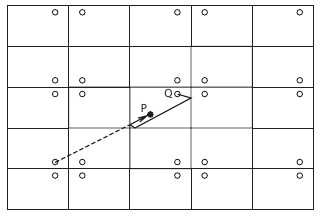
\includegraphics[scale=1]{pics/room1}
\caption{Замощение плоскости отражёнными копиями комнаты.}
\label{pic:room1}
\end{figure}

На полученной картинке каждый выстрел представляется отрезком от какой-то копии точки $Q$ до точки $P$.
Каждый раз, когда такая линия пересекает границу между прямоугольниками, лазерный луч отражается от стенки.
На рисунке показана одна из таких (пунктирных) линий; сплошная линия --- это путь соответствующего луча.

Нам надо перехватить любой выстрел.
Для этого сделаем копию плоскости, показанной на рис. \ref{pic:room1}, прикрепим её к плоскости в точке $P$, и уменьшим эту копию вдвое по вертикали и горизонтали.
Копии точки $Q$ на уменьшенной плоскости будут подходящими позициями охранников.
Они выполняют свою задачу, ведь они лежат ровно на полути между копиями пушки исходного замощения и вами.

На рис. \ref{pic:room2} уменьшенная копия изображена серым цветом, и указаны некоторые воображаемые пути лазера; можно видеть, что на полпути они проходят через соответствующие более мелкие точки серой сетки.

\begin{figure}[t!]
\centering
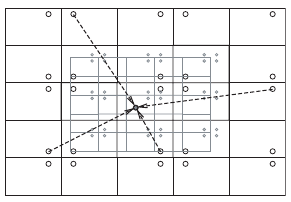
\includegraphics[scale=1]{pics/room2}
\caption{Уменьшенная копия плоскости с точкой $P$ наложенной на себя.}
\label{pic:room2}
\end{figure}

\begin{figure}[b!]
\centering
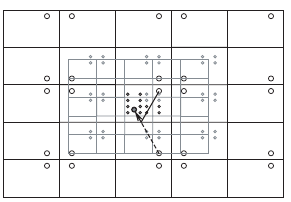
\includegraphics[scale=1]{pics/room3}
\caption{Позиции телохранителей в исходном прямоугольнике.}
\label{pic:room3}
\end{figure}

Конечно, таких точек бесконечно много, но мы утверждаем, что все они являются отражениями набора из 16 точек в исходной комнате.
Четыре из них уже находятся в исходной комнате.
Четыре точки в комнате слева от исходной можно отразить обратно, получив четыре новые точки; аналогично для комнаты выше исходной.
Наконец, четыре точки в комнате \emph{выше и слева} от исходной комнаты могут быть отражены дважды, и так мы получим последние четыре точки в исходной комнате.
На рис.~17 к исходной серой четвёрке точек добавлены двенадцать новых чёрных,
а также показан воображаемый путь лазера и его настоящий путь, проходящий через одну из новых точек.

Поскольку каждая комната выглядит точно так же, как и исходная, или одна из трёх других, которые мы только что рассмотрели, все позиции охранников в плоскости являются отражениями описанных шестнадцати точек в исходной комнате.
Поскольку каждая линия от копии $Q$ проходит через отражённого охранника, фактический выстрел попадает в поставленного охранника на полпути (если не раньше) и поглощается.

Если выбрать местоположения точек $P$ и $Q$ специальным образом, то позиции некоторых охранников совпадут, но в общем случае потребуется полный набор из шестнадцати.

\begin{addedbytheeditors}
Возможно, проще разобрать сначала задачу на плоском торе (то есть в прямоугольнике со склеенными противоположными сторонами).
Убедиться, что в этом случае достаточно четырёх охранников, а потом свести   задачу про прямоугольник к четырём задачам о торе.

Если вам понравилась задача, попробуйте расставить конечное число охранников произвольно близко к точке $P$.\pr
\end{addedbytheeditors}



\subsubsection*{Ящик в ящике}

Эту замечательную головоломку мне подкинул Энтони Квас (Университет Виктории), который услышал её и приведённое ниже решение от Исаака Корнфельда, профессора Северо-Западного университета (Иллинойс).
Корнфельд узнал о ней много лет назад в Москве.

Пусть $B_\varepsilon$ --- $\varepsilon$-окрестность параллелепипеда $B$;
другими словами, это множество всех точек в пространстве, находящихся на расстоянии $\varepsilon$ или меньше от какой-либо точки $B$.
Если $B$ имеет размеры $a \z\times b \z\times c$, то множество $B_\varepsilon$ выглядит как параллелепипед $(a + 2\varepsilon) \z\times (b + 2\varepsilon) \z\times (c + 2\varepsilon)$ с закруглёнными краями и углами.
Точный объём $B_\varepsilon$ будет равен
$abc$ (объем $B$)
плюс $2ab\varepsilon + 2ac\varepsilon + 2bc\varepsilon$ (объем пластин, добавленных к шести граням)
плюс $4a\pi\varepsilon^2 /4 + 4b\pi\varepsilon^2 /4 + 4c\pi\varepsilon^2 /4$ (объем 12-ти штапиков вдоль рёбер --- каждый с поперечным сечением в виде четверти круга),
плюс $4\pi\varepsilon^3 /3$, так как восемь осьмушек, добавленных к углам, образуют целый шар.
Всего получим
\[V(B_\varepsilon)=\tfrac43\pi\varepsilon^3+(a+b+c)\pi\varepsilon^2+2(ab+bc+ca)\varepsilon+abc.\]

Изобразить $B_\varepsilon$ довольно сложно, поэтому мы спустимся на плоскость;
на рис. \ref{pic:box}, показано как выглядит $B_\varepsilon$ для прямоугольника $B$ размера $a \times b$.
Формула для площади $B_\varepsilon$ будет:
\[S(B_\varepsilon)=\pi\varepsilon^2+2(a+b)\varepsilon+ab.\]

\begin{figure}[ht!]
\centering
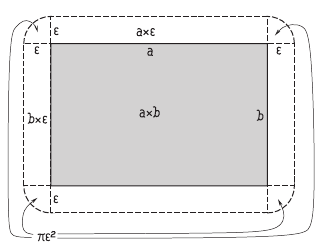
\includegraphics[scale=1]{pics/box}
\caption{$\varepsilon$-окрестность прямоугольник $a \times b$.}
\label{pic:box}
\end{figure}

Вернёмся в трёхмерное пространство.
Если ящик $A$ (с размерами, скажем, $a'\times b'\times c'$) находится внутри ящика $B$, то $A_\varepsilon$ также находится внутри $B_\varepsilon$ для любого $\varepsilon > 0$.
Следовательно, $V(A_\varepsilon ) \z< V(B_\varepsilon)$.
Однако, если выбрать \emph{огромное} $\varepsilon$, то доминирующим членом в разнице их объёмов станет
\[(a+b+c)\pi\varepsilon^2-(a'+b'+c')\pi\varepsilon^2\]
Этот член обязан быть неотрицательным, значит, ящик $B$ дороже чем~$A$.

Эта задача появлялась на Турнире городов 1998 года (5-я задача основного варианта).
Предложенное там решение было другим.
Оно принадлежало Андрею Сторожеву, выходцу из России, который сейчас работает в Австралийском Математическом Фонде.
Решение Сторожева основано на наблюдении, что площадь поверхности внутреннего ящика $A$ должна быть меньше, чем у  $B$.
Это можно увидеть, спроецировав каждую грань $A$ наружу перпендикулярно самой себе и посмотрев на покрытые части поверхности $B$.
Утверждение следует из того, что эти 6 частей не пересекаются, и каждая не меньше соответствующей грани $A$.

Сравнение площадей записывается алгебраически 
\[2a'b'\z+2b'c'\z+2c'a' \z< 2ab\z+2bc\z+2ca\] 
и мы также знаем, что $a'^2\z+b'^2\z+c'^2\z<a^2\z+b^2\z+c^2$, сравнивая диагонали двух ящиков.
Сложив эти два неравенства, получаем 
\[(a'+b'+c')^2<(a+b+c)^2\]
--- готово!

\begin{addedbytheeditors}
Приведённое рассуждение и несколько его вариаций были опубликованы Александром Шенем в 1999 году \cite{shen}.
Заметим, что оно влечёт требуемое неравенство для всех параллелепипедов (не обязательно прямоугольных): если один параллелепипед содержит другой, то сумма рёбер внешнего не меньше суммы рёбер внутреннего.

В книге~А. К. Толпыго \cite{Tolpygo2010} приводится ещё одно решение:
предлагается рассмотреть $9$ длин проекций рёбер внутреннего параллелепипеда на рёбра внешнего.
Сумма трёх проекций любого ребра не меньше, чем само ребро,
а сумма трёх проекций на данное ребро внешнего параллелепипеда не больше длины этого ребра.
Отсюда видно, что сумма рёбер внутреннего параллелепипеда не больше суммы девяти проекций, которая (в свою очередь) не превосходит суммы рёбер внешнего параллелепипеда.

Саму задачу можно воспринимать как рекламу \emph{смешанным объёмам} --- замечательному инструменту в исследовании выпуклых тел.
С ним можно познакомиться по классической книге Ю. Д. Бураго и В. А. Залгаллера \cite{burago-zalgaller}.

То, что объём $\varepsilon$-окрестности любого выпуклого тела (не обязательно параллелепипеда) выражается многочленом, было замечено Якобом Штейнером \cite{steiner}.
Коэффициенты этого многочлена (с точностью до множителя) --- это так называемые \emph{поперечные меры} --- полезные характеристики тела.

В частности, наша задача обобщается следующим образом: если одно выпуклое тело содержится в другом, скажем, $K'\subseteq K$,
то первая поперечная мера $K'$ не превосходит первой поперечной меры $K$.
То же верно и для остальных поперечных мер, но доказательство основано на другой идее.
В размерности три получаем лишь, что объём и площадь поверхности $K'$ не превосходит соответственной характеристики $K$, однако в старших размерностях дело становится интересней.

Первая поперечная мера также равна средней длине проекции тела на случайную прямую (отсюда название).
Ясно, что если одно тело содержится в другом, то тоже верно для всех его проекций.
Так получается другой вариант доказательства, также приведённый в статье Шеня \cite{shen}.
%В терминах поперечных мер решение исходной задачи можно получить из того, что проекция параллелепипеда на случайную прямую (1-мерная поперечная мера параллелепипеда) пропорциональна сумме его измерений.
%Это решение было опубликовано в 1999 году Александром Шенем \cite{shen}.
\pr
\end{addedbytheeditors}

%В статье  приведено и другое решение, основанное на вероятностных соображениях (согласно смутным воспоминаниям автора, это решение ему рассказал кто-то другой).
%Пусть $X$~---  выпуклое множество в $\mathbb{R}^3$.
%Рассмотрим случайную прямую $\ell$ в $\mathbb{R}^3$. Ортогональная проекция $X$ на $\ell$ является отрезком. Обозначим через $d(X)$ ожидаемую длину этого отрезка.
%Если $X_m$ отрезок длины $m$, то $d(X_m)$ пропорционально $m$, т. е. $d(X_m) =km$ для некоторой константы $k>0$.
%(На самом деле $k =1/2$, но точное значение здесь не имеет значения.)
%Пусть теперь $X$~--- ящик размерами $a\times b\times c$. Для каждой прямой $\ell$ проекция $X$ на $\ell$ имеет длину $p_a + p_b+p_c$, где $p_a$, $p_b$, $p_c$~---  проекции отрезков рёбер коробки с длинами $a$, $b$, $c$ соответственно. Усредняя, получаем, что $d(X) = k(a + b + c).$
%Если ящик $X'$ размерами $a'\times b'\times c'$ находится внутри $X$, то проекция $X'$ на произвольную прямую $\ell$ будет покрыта проекцией $X$ на $\ell$, поэтому $d(X')\le d(X)$.
%Объединив это наблюдение с предыдущим, мы видим, что $a'+b'+c'\le a+b+c.$ 
%А: я закоментил эту часть так как здесь повторялось то, что уже сказано.

\chapter{Пути и графы}

\setlength{\epigraphwidth}{.53\textwidth}
\epigraph{Человеку приятен небольшой беспорядок в своей геометрии.}{--- Луи де Берниер (1954---)}

%Человеку нравится неаккуратность в его геометрии

%Louis de Bernieres (2012). “Corelli's Mandolin: A Novel”, p.256, Vintage:

%The captain clicked his tongue disapprovingly, `Symmetry is only a property of dead things.
%Did you ever see a tree or a mountain that was symmetrical?
%It's fine for buildings, but if you ever see a symmetrical human face, you will have the impression that you ought to think it beautiful, but that in fact you find it cold.
%The human heart likes a little disorder in its geometry, Kyria Pelagia.
%Look at your face in a mirror, Signorina, and you will see that one eyebrow is a little higher than the other, that the set of the lid of your left eye is such that the eye is a fraction more open than the other.
%It is these things that make you both attractive and beautiful, whereas . . . otherwise you would be a statue. Symmetry is for God, not for us.'

%– Симметрия свойственна только мертвому. Вы когда-нибудь видели симметричные дерево или гору? Это хорошо для строений, а вот если бы вы увидели симметричноечеловеческое лицо, у вас бы сложилось впечатление, что его только полагается считать красивым, а на самом деле оно холодное. Человеческой душе нравится, чтобы в ее геометрии был небольшой беспорядок, кирья Пелагия. Посмотрите на себя в зеркало, синьорина, и вы увидите, что одна бровь у вас немного выше другой, что левое веко делает этот глаз чуточку шире. Но вы привлекательны и красивы, несмотря на... а иначе вы были бы статуей. Симметрия – для Господа, не для нас.

Спустимся в одномерный мир --- к кривым, которые вам должны быть известны, и графам, о которых вы, возможно, не слышали.
Граф это набор точек, называемых вершинами, некоторые пары из которых образуют \emph{рёбра}.
Часто вершины графа изображаются точками на плоскости, а его рёбра — отрезками или кривыми, соединяющими одну свою вершину с другой.
Если при этом можно обойтись без пересечений рёбер друг с другом, то граф называется \emph{планарным}.

\subsection*{Укрепление сетки}\rindex{Укрепление сетки}

Дана сетка размера $n \times n$ из стержней единичной длины, шарнирно соединённых в концах.
Разрешается укрепить некоторый набор $S$ клеток диагональными скобами (длиной $\sqrt{2}$).

Какие наборы $S$ достаточны для того, чтобы сетка стала жёсткой на плоскости?

\begin{figure}[ht!]
\centering
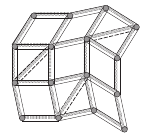
\includegraphics[scale=1]{pics/lattice1}
\caption{Недоукреплённая сетка.}
\label{pic:lattice1}
\end{figure}

На рис. \ref{pic:lattice1} показана недоукреплённая сетка $3 \times 3$.

\subsection*{Путешествие по острову}\rindex{Путешествие по острову}

Алоизий катается по острову на своём прекрасном автомобиле.
Известно, что на каждом перекрёстке острова сходится ровно три (двусторонние) улицы.
Алоизий придерживается следующего правила:
начав с какого-то перекрёстка, он едет в произвольном направлении, на следующем перекрёстке он поворачивает направо, затем налево,
направо,
налево
и так далее.

Докажите, что рано или поздно Алоизий вернётся на перекрёсток, с которого начал.

\parit{Примечания.}
Граф, в котором к каждой вершине подходят ровно три ребра, называется \emph{кубическим}.
В нашем графе есть понятия \emph{право} и \emph{лево},
для этого достаточно изобразить граф на плоскости, с рёбрами (улицами) образованы кривыми.
При этом не обязательно требовать, чтобы граф был \emph{планарным};
можно разрешить мосты и туннели, то есть места, где ребра проходят друг над другом.

\subsection*{Провода под Гудзоном}\rindex{Провода под Гудзоном}

Пятьдесят одинаковых проводов проведены под рекой Гудзон.
Требуется определить все пары концов на обоих берегах.
Для этого разрешается замыкать любые пары проводов на западном берегу, а на восточном проверять концы;
другими словами, вы можете выяснить, какие пары проводов на восточном берегу соединены на западном.

Сколько потребуется поездок через Гудзон, чтобы справиться с этим заданием?

\subsection*{Жуки на четырёх прямых}\rindex{Жуки на четырёх прямых}

Даны четыре прямые на плоскости в общем положении (никакие две не параллельны и никакие три не пересекаются в одной точке).
Вдоль каждой прямой ползёт жук-призрак с постоянной скоростью (скорости разных жуков могут быть разными).
Будучи призраками, при встрече жуки продолжают ползти сквозь друг друга.

Докажите, что если было пять из всех шести возможных встреч,
то была и шестая.

\medskip

Ну раз уж мы начали про жуков...

\subsection*{Пауки на кубе}\rindex{Пауки на кубе}

Три паука и муравей бегают по рёбрам куба.
Каждый паук бегает в три раза медленней муравья.
Докажите, что пауки смогут поймать муравья.

\medskip

Следующая головоломка подведёт нас к прекрасной теореме теории графов.

\subsection*{Вменяемые мыслители}\rindex{Вменяемые мыслители}\label{Вменяемые мыслители}

Жители Перевёртовска каждую неделю встречаются и обсуждают городские дела, в частности, поддерживать ли им строительство нового торгового центра.
Во время встреч каждый перевёртовец обсуждает этот вопрос со всеми своими друзьями (у каждого их нечётное число по какой-то причине) и на следующий день (если требуется) он меняет своё мнение о торговом центре так, чтоб оно совпадало со мнением большинства его друзей.

Докажите, что с какого-то момента каждую \emph{вторую} неделю у каждого перевёртовца будет то же самое мнение.

\parit{Примечания.}
Очевидно, что рано или поздно произойдёт зацикливание, ведь существует только конечное число наборов мнений (их $2^n$, если в городе $n$ жителей). 
В данном случае утверждается, что период цикла должен быть $2$ (или $1$).
С чего бы это?

\medskip

И под конец задача о ком-то, кто хотел бы остаться на своём графе.

\subsection*{Лемминг на шахматной доске}\rindex{Лемминг на шахматной доске}\label{Лемминг на шахматной доске}

На каждой клетке шахматной доски $n\times n$ поставлена стрелка к одной из его восьми соседних клеток (или за пределы доски, если это клетка на краю).
Однако направления стрелок в соседних клетках (включая диагональные) могут различаться не более чем на 45 градусов.

Лемминг начинает свой путь с центральной клетки, и идёт по стрелкам.
Придётся ли ему упасть с доски?

\section*{Источники и решения}

\subsubsection*{Укрепление сетки}

Эту интересную (и, возможно, практически полезную) головоломку подкинул мне геометрический гуру Боб Коннелли из Корнеллского университета; она основана на работе Этана Болкера и Генри Крапо \cite{8}.


\begin{figure}[ht!]
\centering
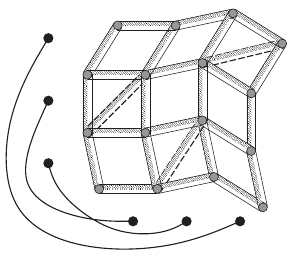
\includegraphics[scale=1]{pics/lattice2}
\caption{Недоукреплённая сетка и её граф.}
\label{pic:lattice2}
\end{figure}

\begin{figure}[t!]
\centering
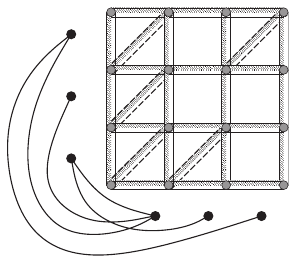
\includegraphics[scale=1]{pics/lattice3}
\caption{Полностью укреплённая сетка и её граф.}
\label{pic:lattice3}
\end{figure}

Задачу полезно перевести на язык графов, но не самым очевидным образом (не нужно смотреть на граф с вершинами в сочленениях стержней).
Предположим, что скобы расставлены.
Рассмотрим граф $G$, вершины которого соответствуют строкам и столбцам сетки.
Каждое ребро в $G$ соответствует строке и столбцу, пересекающимся по закреплённой клетке, так что число рёбер в $G$ равно числу скоб.
Сетка с рис. \ref{pic:lattice1}, показана снова на рис. \ref{pic:lattice2}, но уже с её графом.

Предположим, что некоторая строка смежна в $G$ с некоторым столбцом.
Тогда вертикальные стержни этой строки перпендикулярны горизонтальным стержням этого столбца.
Если $G$ --- связный граф (то есть любые две вершины в нём соединяются путём), то все горизонтальные стержни перпендикулярны всем вертикальным.
Таким образом, все горизонтальные стержни параллельны друг другу,
также параллельны и все вертикальные.
Теперь ясно, что сетка жёсткая.

С другой стороны, предположим, что граф несвязен.
Пусть $C$ --- его \emph{компонента}, то бишь связный кусок $G$, рёбра из которого не идут к остальным вершинам $G$.
Тогда ничто не мешает любому вертикальному стержню в строке $C$ или любому горизонтальному стержню в столбце $C$ крутиться относительно остальных стержней в сетке.

Таким образом, жёсткость в точности означает связность $G$.
Поскольку $G$ имеет $2n$ вершин, если он связен, то у него как минимум $2n - 1$ ребро
(если это для вас новость, то попробуйте доказать индукцией по числу вершин).
Следовательно, чтобы сделать сетку жёсткой, нужно как минимум $2n - 1$ скоб.

Обратите внимание, что скобы нельзя ставить где попало.
На рисунке 21 показана полностью закреплённая сетка $3 \times 3$, и её граф.
Попробуйте подсчитать сколькими способами можно укрепить сетку $3 \times 3$ используя минимальное число скоб  (пять штук).
Есть теорема в теории графов о том, что у каждого связного графа есть \emph{остовое дерево}; то бишь связный подграф с минимальным числом рёбер.
Она позволяет сделать следующий вывод: \emph{если закреплено больше чем $2n - 1$ клеток и сетка жёсткая, то можно удалить все кроме $2n - 1$ скоб, сохраняя жёсткость.}

\subsubsection*{Путешествие по острову}

Вариант этой головоломки был взят на веб-страницу «The Puzzle Toad» \cite{bohman-pikhurko-frieze-sleator} из упомянутой выше книги «Московские математические олимпиады» Г. А. Гальперина и А. К. Толпыго \cite{23}.

Между перекрёстками текущее состояние Алоисия характеризуется тройкой, состоящей из ребра, на котором он находится, направления движения и типа последнего поворота (вправо или влево).
Эта тройка полностью определяет будущие и прошлые положения Алоисия.
Поскольку таких троек конечное число, настанет момент, когда Алоисий впервые попадёт в одну и ту же тройку, и это может произойти только на его стартовом ребре!

%\begin{addedbytheeditors}
%\textbf{Редакторам:} Добавил фразу про будущее и прошлое
%\end{addedbytheeditors}


\subsubsection*{Провода под Гудзоном}

Вариант этой головоломки рекламировал Мартин Гарднер,
иногда её называют задачей Грэма --- Нолтона.
Для электриков это просто задача идентификации кабельных линий.
В версии Гарднера можно было замыкать любое число проводов на любом берегу и также проверять их на любом берегу.
Следующее решение было предложено Роландом Спрэгой в его книге \cite{54}, а также в недавней статье трёх молодых специалистов по информатике Навина Гойала, Сачина Лодхи и Муту Мутукришнана \cite{33}.
Оно удовлетворяет нашим дополнительным ограничениям и требует только две операции на каждом конце (таким образом, потребуется три переправы через реку, не считая дополнительной для размыкания проводов перед использованием).
Однако решение не единственное, и если ваше трёхпереправное решение отличается, то оно может быть ни чуть не хуже.

Пометим концы проводов $w_1$, $w_2, \dots, w_{50}$ на западном берегу
и $e_1, \dots, e_{50}$ на восточном. %??? n>50
При первом посещении западного берега соединим $w_1$ с $w_2$, $w_3$ с $w_4$, $w_5$ с $w_6$ и так далее, но последнюю пару $w_{49}$ и $w_{50}$ соединять не будем.
Затем будем изучать провода на восточном берегу, пока не найдём все пары.
Возможно мы узнали, что $e_4$ соединён с $e_{29}$, $e_2$ с $e_{15}$, $e_8$ с $e_{31}$ и так далее, а концы $e_{12}$ и $e_{40}$ остались без парных.
Затем мы едем на западный берег, рассоединяем все пары и соединяем $w_2$ с $w_3$, $w_4$ с $w_5$ и так далее, оставив $w_1$ и $w_{50}$ без соединения.
Опять изучаем восточные концы, пока не найдём все пары.
Продолжая пример, пусть $e_{12}$ соединён с $e_{15}$, $e_{29}$ с $e_2$, и $e_4$ с $e_{31}$, а концы $e_{40}$ и $e_8$ остались без парных.

Удивительно, но этой процедуры достаточно!

Тот восточный конец провода, который был спарен в первый раз, но не во второй (в нашем примере это $e_8$), должен соответствовать $w_1$.
Следовательно, восточный конец провода, с которым $e_8$ был спарен в первый раз (у нас это $e_{31}$), должен соответствовать $w_2$.
Но тогда $w_3$ должен соответствовать восточному концу провода, с которым $e_{31}$ был спарен во второй раз, а именно $e_4$.
Продолжая таким образом, мы находим, что $w_4$ соответствует $e_{29}$ (парному к $e_4$ на первом круге), $w_5$ соответствует $e_2$ (парному к $e_{29}$ на втором круге) и так далее.
В конце концов мы видим, что $w_{50}$ соответствует $e_{40}$.

Если число проводов (скажем, $n$) нечётно, то в первый раз можно оставить без пары только $w_n$, а во второй --- $w_1$, и всё сработает примерно так же.

\subsubsection*{Жуки на четырёх прямых}

Эта головоломка мне досталась от Мэтта Бэйкера из Технологического института Джорджии.
Иногда её называют \emph{задачей четырёх путешественников};
её можно увидеть на веб-сайте «Cut the knot» \cite{cut-the-knot}.

В наиболее изысканном решении, которое мне известно, требуется подняться из плоскости в пространство, добавив ось времени.
Предположим, что все встречаются, кроме (возможно) третьего и четвёртого жука.
Проведём ось времени перпендикулярно плоскости с жуками, и пусть $g_i$ --- график $i$-го жука в пространстве.
Поскольку каждый жук ползёт с постоянной скоростью, каждый такой график является прямой;
его проекция на плоскость с жуками --- это та самая прямая, по которой ползёт жук.
Два жука встречаются тогда (и только тогда) когда их графики пересекаются.

Прямые $g_1$, $g_2$ и $g_3$ находятся в одной плоскости, так как они попарно пересекаются.
То же самое относится и к тройке  $g_1$, $g_2$ и $g_4$.
Следовательно, все четыре графика лежат в одной плоскости.
Конечно же, $g_3$ и $g_4$ не параллельны, ведь не параллельны их проекции.
Таким образом, эти две прямые обязаны пересечься в своей плоскости,
а это и значит, что третий жук встретит четвёртого.

\subsubsection*{Пауки на кубе}

У этой головоломки тот же источник, что и у «Путешествия по острову» выше.

\begin{figure}[ht!]
\centering
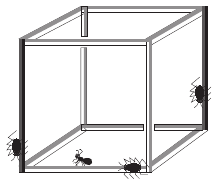
\includegraphics[scale=1]{pics/cube}
\caption{Два чёрных ребра под контролем, и муравей ловится в серой зоне.}
\label{pic:cube}
\end{figure}

Для поимки муравья можно заставить двух пауков охранять по одному ребру.
Для охраны ребра $PQ$ паук сначала выгоняет с него муравья, если это необходимо, а затем бегает по ребру так, что он всегда хотя бы в три раза ближе к $P$ (и к $Q$) чем муравей.
Это возможно, ведь если запрещено использовать ребро $PQ$, то путь от $P$ до $Q$ вдоль рёбер куба в три раза длиннее самого ребра.

Если охранять два \emph{противоположных} ребра (другие варианты также работают), то в оставшейся части куба без этих рёбер и их концов не будет циклов (см. рис. \ref{pic:cube}).
Значит, третий паук сможет преследовать муравья до конца охраняемого ребра, где тот встретит свою грустную участь.

\subsubsection*{Вменяемые мыслители}

Эту головоломку мне предложил Саша Разборов из Института перспективных исследований;
с его слов я знаю, что она была кандидатом на Международную математическую олимпиаду, однако была отвергнута как слишком сложная.
Она была рассмотрена и решена в статье Э. Голеса и Х. Оливоса \cite{31}.

Нам надо доказать, что мнения установятся или будут меняться с периодом в пару недель.
Будем думать о каждом знакомстве как о паре стрелок, по одной в каждом направлении.
Назовём стрелку \emph{обидной}, если мнение перевёртовца в начале стрелки отличается от мнения его знакомого на конце стрелки на \emph{следующей неделе}.

Рассмотрим стрелки, выходящие от некого превёртовца Клайда на неделе $t - 1$, во время которой Клайд выступает (скажем) за торговый центр.
Предположим, что из них $m$ обидных.
Если Клайд все ещё (или снова) за торговый центр на неделе $t + 1$, то число, скажем $n$, обидных стрелок, указывающих на Клайда на неделе $t$, будет в точности равно~$m$.

Однако, если Клайд против торгового центра на неделе $t + 1$, то $n$ будет строго меньше $m$, так как большинство его друзей были против торгового центра на неделе $t$.
Следовательно, большинство стрелок от Клайда были обидными на неделе $t - 1$, а на неделе $t$ только меньшинство обидных стрелок направлены к Клайду.

Всё это остаётся верным и если Клайд был против торгового центра на неделе $t - 1$.

Но вот какое дело: \emph{каждая} стрелка начинается у \emph{кого-то} на неделе $t - 1$ и заканчивается у кого-то на неделе $t$.
Таким образом, общее число обидных стрелок между неделями $t - 1$ и $t$ не увеличивается и даже строго уменьшается, за исключением случая, когда каждый перевёртовец имел такое же мнение на неделе $t - 1$, как и на неделе $t + 1$.

Общее число обидных стрелок в данную неделю не может бесконечно уменьшаться.
В итоге оно достигнет значения, с которого уже не опустится.
В этот момент каждый перевёртовец либо сохранит своё мнение навсегда, либо будет менять его туда-сюда каждую неделю.

\medskip

Задачу можно значительно обобщить, например, добавив веса вершинам (это означает, что мнения одних ценнее, других), разрешив петли (то есть разрешив учитывать своё текущее мнение), введя механизмы разрешения конфликтов и даже установив различные пороги для смены мнений «за» и «против».

\subsubsection*{Лемминг на шахматной доске}

Эту замечательную головоломку придумал Кевин Пурбху, ещё будучи старшеклассником в Торонто.
С тех пор он защитил диссертацию по математике в Университете Калифорнии в Бёркли и
сейчас проходит постдоктурантуру в Университете Британской Колумбии,
занимаясь чем-то под названием \emph{тропическая геометрия}.
Сам я узнал головоломку от Рави Вакила из Стэнфордского университета.

Лемминг действительно обречён.
Один из способов это понять (найденный независимо Вакилом и мной) --- представить, что лемминг может перемещаться на любую соседнюю клетку, но должен при этом повернуться в направлении стрелки, которую он там обнаружит.
Лемминг не может повернуться на 360°, обойдя цикл;
ведь если бы он мог, то можно уменьшать такой цикл, пока не придём к противоречию.
Но настоящий лемминг, если он хочет остаться на доске, в конечном итоге должен обойти цикл, и когда это произойдёт, ему придётся повернуть на 360°.

Собственное решение Пурбху, с его школьных лет, использует индукцию.
Если лемминг остаётся на доске, он, как мы уже отметили, должен будет обойти цикл.
Пусть $C$ --- цикл наименьшей возможной площади (на любой доске), на котором это может произойти; будем считать, что лемминг обходит его по часовой стрелке.
Обрежем всю доску до $C$ и того, что он окружает.
Затем повернём все стрелки на 45° по часовой стрелке.
Это приведёт к меньшему циклу!

\begin{addedbytheeditors}
Нехитрая техника, сводит головоломку к следующему утверждению про векторные поля: \emph{Векторное поле без нулей на плоскости не имеет замкнутых интегральных линий.}
Решение получится сложней, но возможно полезней.\pr
\end{addedbytheeditors}

\chapter{Игры и стратегии}

% читает Устинов

\setlength{\epigraphwidth}{.63\textwidth}
\epigraph{Если не найти игры, в которую стоит играть, тогда придумайте новую. 
}{— Энтони Д'Анджело}%, «Справочник абитуриента»}

Даже если бы мы не играли в игры, нам пришлось бы их придумать.
Ведь про многие математические задачи удобно думать как об играх.
Мы уже обсудили несколько задач о поиске лучшей стратегии, и сейчас обсудим ещё несколько.

Начнём с простого вопроса о покере --- игре, в которую люди играют всерьёз.

\subsection*{Покер: быстрый вопрос}\rindex{Покер: быстрый вопрос}

Какой фул-хаус самый лучший?

\parit{Примечания.}
Можно считать, что вы играете в обычный покер \emph{стад} обычной колодой с пятью партнёрами, а Господь Бог оказался вашим должником.
В результате у вас есть право на фул-хаус --- можно получить любой фул-хаус, какой только пожелаете.
Какой лучше всего выбрать?

\subsection*{Восстановление многочлена}\rindex{Восстановление многочлена}

Дельфийский оракул загадал многочлен $p$ с неотрицательными целочисленными коэффициентами (от одной переменной).
Если назвать любое целое число $x$, то оракул выдаст значение $p(x)$.

Сколько запросов нужно сделать, чтобы найти многочлен $p$?

\subsection*{Спасите наши души}\rindex{Спасите наши души}

Дан лист бумаги с рядом из $n$ пустых клеток.
Тристан и Изольда ходят поочерёдно, записывая по букве $S$ или $O$ в незанятую клетку.
Побеждает тот, кто первым напишет $SOS$ в последовательных клетках.
Для каких значений $n$ у второго игрока (Изольды) есть выигрышная стратегия?

\subsection*{Пасьянс с шарами}\rindex{Пасьянс с шарами}

Перед вами урна с некоторым числом зелёных и красных шаров (по крайней мере, по одному каждого цвета).
На первом раунде вы вытаскиваете шар за шаром вслепую (всегда случайным образом), пока не вытянете шар другого цвета; этот шар затем возвращается в урну.

На втором и последующих раундах процесс повторяется, и продолжается пока урна не опустеет.
Если последний вытянутый шар зелёный, то вы победили.

Сколько зелёных и красных шаров следует положить в урну, чтобы максимизировать вероятность выигрыша?

\subsection*{Пиратская демократия}\rindex{Пиратская демократия}

Сотня пиратов на корабле захватила сундук с золотыми монетами и решила поделить их демократически.
Каждый пират, по порядку ранга от капитана до самого младшего, вносит предложение, кто и сколько монет получит.
Все пираты, включая того, кто выдвигает предложение, голосуют.
Для принятия предложения достаточно половины голосов.
В этом случае монеты распределяются соответственно, и процесс завершается.
Если же предложение отвергнуто, то предлагавшего выкидывают за борт, и далее предложение вносит следующий по рангу.

Учтите, что пираты коварны, жадны, осторожны, мыслят очень логично и все они это отлично понимают.
Главное для них --- не попасть за борт.
Если у пирата нет предпочтений между двумя вариантами, то он действует непредсказуемо.

Сколько монет должно быть в сундуке, чтобы капитан смог гарантированно выжить?

\subsection*{Волшебные рамки}\rindex{Волшебные рамки}

Дана обычная красно-чёрная шахматная доска $8 \times 8$ и две \emph{волшебные рамки},  $2 \times 2$ и $3 \times 3$.
Если аккуратно приложить такую рамку к сетке шахматной доски, то $4$ или $9$ покрытых клеток тут же сменят цвета.

Возможно ли так достичь всех $2^{64}$ расцветок доски?

\subsection*{Больше рамок на меньшей доске}\rindex{Больше рамок на меньшей доске}

Теперь у нас доска $6 \times 6$, с целым числом в каждой из $36$ клеток.
Разрешается выбрать любой подквадрат $2 \times 2$, $3 \times 3$, $4 \times 4$, $5 \times 5$ или $6 \times 6$ и добавить единицу к каждому числу внутри него.
Можно ли из любой начальной конфигурации достичь конфигурации со всеми числами, кратными $3$?


\medskip

Покер и многие другие игры включают в себя элемент блефа, а он может быть довольно сложной штукой.
В следующей игре мы разберёмся с основами блефа.

\subsection*{Простой блеф}\rindex{Простой блеф}

Рассмотрим следующую простую игру в блеф.
Луиза и Джереми делают начальную ставку по одному доллару каждый.
Далее Луиза берёт карту из перетасованной колоды и смотрит на неё.
Она может поднять ставку на 10 долларов (добавив свои 10 долларов в банк) или оставить ставку как есть.

Если Луиза не поднимает ставку, то она выигрывает банк, если у неё на руках пика, в противном случае --- проигрывает.

Если Луиза поднимает ставку, то Джереми может проверить (добавив свои 10 долларов в банк) или же сбросить свои карты.
Если Джереми сбрасывает карты, то Луиза забирает деньги в банке, тем самым выигрывая доллар Джереми.
Если же Джереми проверяет и у Луизы действительно пика, то Луиза снова забирает банк, на этот раз с 11 долларами Джереми.
Ну а если карта не пика, то банк забирает Джереми.

Кому выгодна такая игра?
А что, если вместо 10 долларов выбрать другое повышение ставки?

\subsection*{Китайский ним}\rindex{Китайский ним}

На столе лежат две кучки бобов.
Алекс должен взять несколько бобов либо из одной кучки, либо по одинаковому числу бобов из обеих.
Затем Бет делает ход по тем же правилам.
Так они чередуют ходы до тех пор, пока один из игроков не выиграет, взяв со стола последний боб.

Какова правильная стратегия в этой игре?
Что если Алекс начинает с кучек с 12\,000 и 20\,000 бобов?
А что если с 12\,000 и 19\,000?

\section*{Источники и решения}

\subsubsection*{Покер: быстрый вопрос}

Этим вопросом меня озадачил Стэн Уэгон, а он нашёл его в книге Аарона Фридланда \cite{18}.

Суть в том, что все \emph{фулл-хаусы} с тремя тузами одинаково сильны, ведь из одной колоды двух таких не набрать.
Однако фулл-хаусы бьются другими комбинациями: любое \emph{каре}, а их 11 штук, и, что важнее для нас, \emph{стрит-флэшами}.
Фулл-хаусы ТТТ99, ТТТ88, ТТТ77 и ТТТ66 выбивают из колоды максимальное число стрит-флэшей.
Каждый туз выбивает два стрит-флэша, и каждая фоска (карта младшего достоинства) выбивает по пять --- всего 16.
Эти фулл-хаусы и являются лучшими.

Если же вы всё равно потребуете ТТТКК, то вас побьют $40 - 9 \z= 31$ стрит-флэшей, или даже $40 - 16 = 24$, если в вашем фулл-хаусе не нашлось всех четырёх мастей.

\subsubsection*{Восстановление многочлена}

Эту загадку мне подкинул Джо Булер (Рид-колледж), который считает, что она должна быть очень древней.

Как вы наверно уже догадались, достаточно двух запросов:
если $p(1)=n$, то коэффициенты не превышают $n$.
Далее можно взять $x = n + 1$, и записать ответ $(n + 1)$-ичной системе счисления.
Получим все коэффициенты многочлена!

Джо отметил, что если бы разрешалось задавать произвольные числа, то было бы достаточно одного запроса $x = \pi$.
Надо думать, что Оракул найдёт способ выдать значение $p(\pi)$ за конечное время;
если же вместо этого он станет выдавать его десятичное разложение по одной цифре,
то вам придётся понять, когда остановиться.

Хельге Тверберг заметил, что эта задача имеет смысл для многочленов с неотрицательными вещественными коэффициентами.
Чтобы восстановить $p$, сначала спросим $p(1)$; если ответ $0$, то $p = 0$ и задача решена.
В противном случае будем стоить \emph{конечные разности}.
Положим $p_0(x) = p(x)$, и определим рекурсивно последовательность многочленов $p_{i+1}(x) = p_i (x+1) - p_i(x)$.
Отметим, что коэффициенты всех $p_i$-х неотрицательны.
За $k$ вопросов мы можем узнать $p(1),\dots,p(k)$,
а из них вычислить $p_{k-1}(1)$.
Наименьшее $k$ при котором мы получим $0$ это $d+2$, где $d$ --- степень $p$.
Как только мы знаем $d$, любых $d+1$ из $d+2$ имеющихся у нас значений $p$ достаточно, чтобы восстановить многочлен.

\subsubsection*{Спасите наши души}

На эту игру указал мне аспирант Рэйчел Эссельштейн.
Вместе с множеством других игр, она обсуждается в книге Тома Фергюсона по теории игр \cite{ferguson}.
Этот вариант игры также предлагался на 28-ой Американской математической олимпиаде 1999 годa.

Вопрос кажется туманным, пока не увидишь следующее.
Единственный способ заставить противника походить так, чтобы выиграть на следующем ходу это заставить его ходить внутрь конфигурации S-пусто-пусто-S (мы её будем называть \emph{ямой}).
Например, Тристан может выиграть, если $n = 7$, поставив $S$ в середину, а затем поставив ещё одну $S$ в конце, подальше от ответного хода Изольды.
Теперь у нас есть яма.
После пары ходов на другой стороне, Изольде придётся сходить в яму и проиграть.

То же самое справедливо для любого нечётного $n$ больше $7$ --- Тристану достаточно поставить $S$, в $4$-х или более клеток от обоих концов, построить яму с одной или другой стороны, а затем ждать.

Если $n$ чётное, то у Тристана нет шансов, ведь Изольде не могут достаться одни ямы --- каждый раз на её ходе у неё нечётное число пустых клеток.
Если же $n$ чётное и большое, то Изольда выигрывает, сыграв $S$ далеко от концов и от первого хода Тристана.
Однако, если Тристан начинает с $O$, то Изольде нельзя поставить $S$ рядом, поэтому потребуется дополнительное место.

В случае $n = 14$, если Тристан поставит $O$ на $7$-ю клетку (нумерация от $1$ до $14$), то лучший ответ Изольды --- $S$ на в позиции $11$ (угроза создать яму с $S$ на $14$-й клетке).
В ответ, Тристан может поставить $O$ на $13$-ю или $14$-ю клетку (или $S$ на $12$-ю). 
Теперь Изольда хотела бы построить яму поставив $S$ на $8$-ю клетку, но ей нельзя, ведь тогда Тристан выиграет, поставив $S$ в $6$-ю позицию.

Таким образом, при $n = 14$ --- ничья;
Изольде нужно, чтобы $n$ было чётным и не менее 16.
В итоге, Тристан выигрывает, если $n$ --- нечётное и не менее $7$,
Изольда --- если $n$ --- чётное и не меньше $16$;
все остальные значения $n$ приводят к ничьей при оптимальной игре.

\subsubsection*{Пасьянс с шарами}

Эту головоломку (немного в другом виде) можно найти в книге Мартина Гарднера \cite[2.16]{30}, однако там ответ дан без доказательства.
Доказательство из статьи \cite{45}, которое там упомянуто, занимает три страницы и слишком техническое и для Гарднеровской книги, и для моей.

К счастью, есть простой способ понять, что вероятность выигрыша всегда равна $1/2$, независимо от соотношения красных и зелёных шаров в урне.
Ниже приведено рассуждение Серджио Харта из Иерусалимского университета, который и обратил моё внимание на эту задачу.

Иногда в анализе случайного процесса лучше переместить случайность в другое место.
В этой задаче полезно (и допустимо) представить, что перед каждым раундом оставшиеся шары случайно упорядочиваются, и после этого выбираются слева на право.
Тогда в последним раунде, все шары одноцветны.
В предыдущем раунде есть шары обоих цветов, но все красные шары стоят слева, а все зелёные справа, или наоборот.
Независимо от числа шаров каждого цвета на этом этапе (или изначально), эти два порядка равновероятны.
Поскольку первый приводит к выигрышу, а второй к проигрышу, получаем, что вероятность выигрыша равна 1/2.

Серджиу заметил, что этот пасьянс в некотором смысле эквивалентен «Потерянному посадочному талону» \cite[стр. ???]{59}.
Хельге Тверберг (Бергенский университет в Норвегии) отметил что есть также не столь хитрое, но вполне изящное решение индукцией по числу шаров.

\subsubsection*{Пиратская демократия}

Мне напомнил об этой старой загадке аспирант Дартмутского университета Джулио Дженовезе.
Как и многие игры, она решается обратным ходом.
Давайте пронумеруем пиратов от младшего к старшему, и пока будем счиать, что у них всего $n$ монет.
Если дело дойдёт до самого младшего $P_1$, то, он конечно же возьмёт всё золото себе.
(Будем надеяться, что в одиночку он сможет довести корабль к пристани!)

Однако, если дело дошло до $P_1$, то оно дошло и до $P_2$, а
$P_2$, конечно же, оставит себе все монеты и проголосует «за», останется в живых, и возглавит корабль.

Далее, если дело дошло до $P_3$, то он купит голос $P_1$ за одну монету, взяв оставшиеся $n - 1$ себе.
Следовательно, наилучшим вариантом для $P_4$ будет подкупить $P_2$ одной монетой ---
этого достаточно, ведь иначе $P_2$ не получит ничего.

$P_5$ нужны уже два голоса, и он получит их отдав по монете $P_1$ и $P_3$ --- этого достаточно.

Уже видна закономерность, и даже есть что доказывать индукцией:
если осталось нечётное число пиратов, то следует предложить по одной монете каждому оставшемуся нечётному пирату (предполагая, что монет хватит);
если же их чётное число, то следует предложить по одной монете каждому оставшемуся чётному пирату.
По предположению индукции, все получающие монеты пираты проголосуют «за», и теперь уже нечего доказывать.

Ну так что там по поводу капитана?
Чтобы точно выжить, ему потребуется 49 монет; дабы предложить по монете всем чётным пиратам ниже 100.

\subsubsection*{Волшебные рамки}

Эту головоломку предложил Эхуд Фридгут из Еврейского университета; это вариация одной из задач, которая появилась на израильском молодёжном математическом соревновании.
В соревновании рамки были размером $3 \times 3$ и $4 \times 4$.
В этом случае подсчёт вариантов говорит, что всех конфигураций цветов достичь невозможно.
Суть в том, что порядок, в котором располагаются рамки, не имеет значения;
достаточно знать какими способами установки рамок мы воспользовались.
У нас есть $5^2$ способов установки рамки $4 \times 4$
и $6^2$ способов установки рамки $3 \times 3$.
Таким образом, всего $2^{25} \times 2^{36} = 2^{61}$ варианта, этого мало.

Однако, в варианте Фридгута, у нас уже $2^{49} \times 2^{36}$ вариантов, и теоретически этого хватает для получения всех $2^{64}$ конфигураций.
Думаете, теперь получится?

\begin{figure}[ht!]
\centering
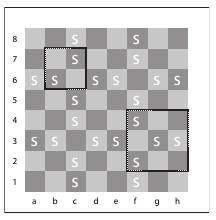
\includegraphics[scale=1]{pics/chess}
\caption{Особые клетки (помечены буквой S) и пара рамок.}
\label{pic:chess1}
\end{figure}

Назовём клетку \emph{особой}, если она находятся в третьей или шестой строке или в третьем или шестом столбце, но не в обоих таких позициях сразу (рис. \ref{pic:chess1}); тогда каждая рамка $2 \times 2$ или $3 \times 3$ покрывает чётное число особых клеток.

Поскольку на доске изначально чётное число чёрных особых клеток, у нас не получится достичь конфигурации, с нечётным  числом чёрных особых клеток.

\subsubsection*{Больше рамок на меньшей доске}

Эту головоломку подкинул мне Джулио Дженовезе, он узнал её от Владимира Чернова, тренеровавшего Джулио к Олимпиаде Патнема; сам Владимир, нашёл её в книге «Новые олимпиады по математике» \cite{markova}.

Как и в предыдущей задаче, нужно найти чудесный инвариант.
Однако начнём с совсем неправильной идеи.

Конечно же, достаточно рассматривать только рамки $2 \times 2$, $3 \times 3$ и $5 \times 5$, ведь из них можно составить все остальные.

Как уже было отмечено, стоит проверить, хватит ли всего того, что \emph{разрешается}, для того чтобы сделать всё, что \emph{нужно}.
Можно думать, что номера на доске это числа по модулю $3$ ($0$, $1$ или $2$, и $2 + 1 = 0$).
Следовательно, нам надо беспокоится о $3^{6^2} = 3^{36}$ возможных конфигурациях.
На каждой клетке доски каждый тип квадрата может быть установлен, не установлен или установлен дважды; установка трижды ничего не даёт.
У нас $5^2$ мест для установки квадрата $2 \times 2$,
$4^2$ для $3 \times 3$
и $2^2$ для $5 \times 5$, так что в общей сложности есть $3^{25} \times 3^{16} \times 3^4 = 3^{45}$ возможных действий, и этого более чем достаточно.
Видимо, многие из этих действий имеют один эффект.
Так или иначе, пока неясно, можем ли мы получить желаемый результат.

Математически говоря, у нас есть линейное отображение из векторного пространства $\mathbb{Z}_3^{45}$ в векторное пространство $\mathbb{Z}_3^{36}$, и мы хотим узнать всё ли покрывает образ.
(Возможность перехода от конфигурации со всеми нулями к любой произвольной конфигурации эквивалентна обратному.)

Если ответ да, то мы способны перейти от всех нулей к конфигурации, где все нули, кроме одной единицы в выбранном месте.
Более того, если такое возможно, то задача решена, ведь можно проделать это для каждого местоположения, которому не хватает единицы, и дважды для каждого местоположения, которому не хватает двойки.
Это напоминает поиск решения (с нуля) для кубика Рубика --- нужны операции, которые мало, что меняют.
Например: начнём с двух диагонально смежных квадратов $3 \times 3$ так, что они перекрываются по квадрату $2 \times 2$.
Теперь, если добавить по два подквадрата $2 \times 2$ в каждый угол квадрата $4 \times 4$ и ещё два центральных квадрата, то всё отменится, кроме двух диагонально противоположных углов квадрата $4 \times 4$.
Таким образом, можно увеличить две позиции, одна из которых находится на трёх шагах от другой по диагонали.

Однако сложно представить, что возможно изменить одно значение в произвольной позиции.
Давайте поменяем подход.
Если это \emph{не так}, то есть невозможно получить любую конфигурацию, тогда должен существовать \emph{инвариант}: некоторое число, связанное с конфигурацией, которое ни один шаг не меняет.
В линейной задаче, подобного рода, этот инвариант сам должен быть линейной функцией.
Это означает, что должно быть два подмножества $A$ и $B$ клеток таких, что если сложить числа в $A$ и прибавить удвоенную сумму чисел в $B$ (в нашей арифметике по модулю $3$ это тоже, что сумма чисел в $A$ минус сумма чисел в $B$), то это даст инвариант.

\begin{figure}[t!]
\centering
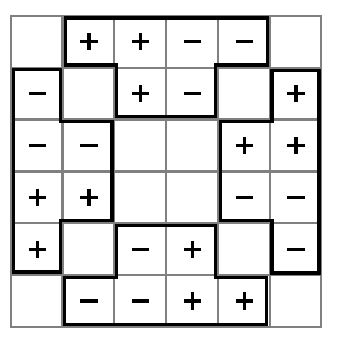
\includegraphics[scale=1]{pics/chess2}
\caption{Множества $A$ и $B$ помеченные знаками $+$ и $-$.}
\label{pic:chess2}
\end{figure}

Построение выше влечёт, что если некоторая позиция находится в $A$, то позиция (всегда есть ровно одна такая) на расстоянии трёх шагов по диагонали должна находиться в $B$, и наоборот.
Исходя из этого наблюдения и зная, что нам нужно в каждом возможной рамке равное число позиций в $A$ и позиций в $B$ (по модулю 3), мы можем найти чудесный узор на рис. \ref{pic:chess2}, в котором точки в $A$ помечены плюсами, а точки в $B$ --- минусами.
И так, мы утверждаем, что сумма значений в позициях $+$, минус сумма значений в позициях $-$, не может измениться.
Отсюда следует, что мы не можем перейти от любой позиции, где это значение не равно $0$, к позиции, в которой все значения равны~$0$.

\subsubsection*{Простой блеф}

Эта головоломка была предложена Джереми Торпом и Луизой Фуше из Калифорнийского технологического института, но похожие игры были известны и раньше.

Отметим, что имея на руках пику, Луиза всегда выгодно поднимать ставку.
Поэтому у неё есть две \emph{чистые} стратегии:
\begin{itemize}
 \item \textbf{честная} --- поднимать ставку только если есть пика.
 \item \textbf{нахальная} --- всегда поднимать ставку.
\end{itemize}
Если Луиза подняла ставку, то у Джереми есть два варианта ответа:
\begin{itemize}
 \item \textbf{робкий} --- сбросить.
 \item \textbf{смелый} --- проверить.
\end{itemize}

Вероятность вытянуть пику составляет $1/4$.
Значит честная стратегия против робкой даёт Луизе 1 доллар $1/4$ времени, и остальное время 1 доллар выигрывает Джереми.
Ожидаемый выигрыш Джереми составит $1/2$ доллара.
Честная стратегия против смелой даёт Луизе 11 долларов, если у неё пика,
a в среднем приносит ей 2 доллара ($\tfrac14 \times 11 - \tfrac 34 \times 1 = 2$).

Далее, нахальная стратегия против робкой приносит Луизе 1 доллар каждый раз,
в то время как нахальная против смелой обходится ей в $5{,}50$ долларов в среднем ($\tfrac34 \times 11- \tfrac14 \times11 = 5{,}50$).
Если вставить эти числа в матрицу игры $2 \times 2$,
то мы не увидим доминирующей стратегии ни для одного из игроков.
Значит, как и следовало ожидать, придётся использовать вероятностную стратегию.

Из работ Джона фон Неймана (ещё до Джона Нэша) известно, что существует \emph{равновесие Нэша} для этой игры --- пара стратегий, при которых ни один из игроков не может улучшить свою стратегию, при условии, что другой игрок не меняет свою.
Посмотрим, что это означает для Луизы: если ей не выгодно переходить к честной или нахальной стратегии, то в среднем ей все равно, проверит ли её Джереми или сбросит.

Предположим, что Луиза решила блефовать с вероятностью $p$, если у неё нет пики.
Против робкой стратегии её ожидаемый выигрыш в среднем составит $\tfrac14 \times 1 + p \times \tfrac34 \times 1 - (1 - p) \times \tfrac34 \times 1 =(\tfrac32p - \tfrac12)$ долларов.
Ну а против смелой, $\tfrac14 \times 11 - p \times \tfrac34 \times 11 - (1 - p) \times \tfrac34 \times 1 \z= (2 - \tfrac{15}2p)$ долларов.

Поскольку Луизе должно быть всё равно, эти две величины должны совпасть, и это даёт $p = 5/18$.
То есть, Луизе следует блефовать $5$ из $18$ раз, когда у неё нет пики и, конечно, всегда повышать ставку, если пика есть.
Её ожидаемый выигрыш независимо от стратегии Джереми будет
\[\frac32\times\frac5{18}-\frac12=2-\frac{15}2\times\frac5{18}=-\frac1{12}\]
долларов.
То есть в среднем Луиза теряет по $\tfrac1{12}$ доллара за игру.

Немного поразмыслив, можно убедиться, что Луизе выгодно увеличить размер повышения ставки,
однако в среднем она останется в минусе, если конечно играют честно.
Причина в том, что если у неё нет пики, то она не может позволить себе блефовать чаще чем один раз из трёх.
Иначе, с точки зрения Джереми, вероятность того, что у неё была бы пика, составила бы не больше половины, и поэтому Джереми мог бы просто всегда проверять.
Луиза в лучшем случае выйдет в ноль, при повышениях ставки, и будет терять по доллару без повышений, и значит в среднем будет проигрывать.
Но если $p < 1/3$, то Луиза проигрывает робкой стратегии Джереми;
в этом случае она чаще теряет свою ставку, чем выигрывает.

Здесь важно, что вероятность вытянуть пику составляет одну четверть.
Если бы шансы были чуть выше (скажем, если в колоде нет дамы червей), то большая ставка повернула бы удачу в сторону Луизы.

Вернёмся к исходным 10 долларам.
Можно вычислить стратегию равновесия для Джереми (хотя нам этого и не требуется).
Предположим, что если Луиза повышает ставку, то Джереми проверяет с вероятностью $q$.
Тогда, против луизиной честной стратегии, он получает $\tfrac34 \times 1 - \tfrac14 \times q \times 11 - \tfrac14 \times (1 - q) \times 1 = \tfrac12 - \tfrac52q$ доларов,
а против смелой стратегии $\tfrac34 \times q \times 11 - \tfrac14 \times q \times 11 - (1 - q) \times 1 = \tfrac{13}2q - 1$ долларов.
Полагая, что эти величины равны, получаем $q = \tfrac3{18}$; то есть, Джереми должен проверять только $\tfrac3{18}$ всего времени.
Подстановка $q = \tfrac3{18}$ обратно в выражения даёт Джереми $\tfrac1{12}$ доллара за игру в среднем, как и должно быть, ведь ровно столько теряет Луиза.

\subsubsection*{Китайский Ним}

Эта игра известна как Китайский ним или как Игра Витоффа;
она появилась в его статье 1907 года \cite{60}.
Игра обсуждается несколько раз в первом и втором томе классической книги Элвина Берлекампа, Джона Конвея и Ричарда  Гая \cite{4}.
Связь с «Надёжными мигалками» приведённой выше была замечена в прекрасной книге Сергея Табачникова \cite{56}.
Однако ни одна из этих книг не приводит вывод стратегии.

Каждая позиция $\{x, y\}$ в игре Алекса и Бет является либо выигрышной, либо проигрышной для игрока, который делает следующий ход, при условии оптимальной игры обоих.
Как и в классическом ниме, проще всего попытаться характеризовать проигрышные позиции, поскольку их меньше.

Как только известны проигрышные позиции, можно вывести правильную стратегию.
Если, например, Алекс находится в выигрышной позиции, то у него должна быть возможность одним ходом перейти к проигрышной позиции для Бет.
Если же Алекс находится в проигрышной позиции, то он может только надеяться на ошибку Бет, или же он по-джентльменски предложит ей сделать первый ход.
Таким образом, стратегия сводится к списку проигрышных позиций.
Но разве здесь нет порочного круга?
Разве нам не нужно знать правильную стратегию, чтобы найти проигрышные позиции?
К счастью, поскольку число бобов всегда уменьшается, мы можем начать снизу и постепенно подниматься вверх.

Любая позиция с одной пустой кучей или с кучами одинакового размера автоматически является выигрышной.
Не сложно понять, что самая простая проигрышная позиция это $\{1, 2\}$.
После этого можно увидеть, что $\{3, 5\}$, $\{4, 7\}$ и $\{6, 10\}$ также проигрышные.
Но где же закономерность?

Пусть $\{x_1 , y_1\}$, $\{x_2 , y_2\},\dots$ будут проигрышными позициями для первого игрока (не считая $\{0, 0\}$);
мы предполагаем что $x_i < y_i$ и $x_i < x_j$ при $i < j$.
Заметим, что $x_i \ne x_j$ для $i \ne j$, ведь если $x_i = x_j$ то Алекс мог бы сделать ход, от большего из $y_i$ и $y_j$ к меньшему, оставляя Бет в проигрышной позиции --- противоречие.

Немного поразмыслив, приходим к выводу, что если известны все проигрышные позиции от $\{x_1 , y_1\}$ до $\{x_{n-1}, y_{n-1}\}$, то $x_n$ есть наименьшее положительное число, которого нет среди чисел из $\{x_1, \dots , x_{n-1}\} \z\cup \{y_1, \dots , y_{n-1}\}$, а $y_n = x_n + n$.
Заметим, что в этом случае $y_n$ превосходит любое число из $\{x_1, \dots , x_{n-1}\} \cup \{y_1, \dots , y_{n-1}\}$.

Доказательство ведётся индукцией по $n$.
Мы уже знаем, что $x_n$ не может быть среди чисел в $\{x_1, \dots , x_{n-1}\} \cup \{y_1, \dots , y_{n-1}\}$, а также, что не может быть более одного $y_n$, который соответствует этому $x_n$.
Остаётся показать, что позиция $\{x_n, y_n\}$ проигрышная.

Если $\{x_n, y_n\}$ была бы выигрышной, то из неё можно было бы прийти в $\{x_i, y_i\}$ для некоторого $i < n$; но такой позиции нельзя достичь уменьшив меньшую кучу или уменьшив обе кучи на одинаковое число бобов, ведь это сделало бы разницу между двумя кучами $n$ или больше.
Также нельзя её достичь, уменьшив б\'{о}льшую кучу, ведь тогда был бы ещё один игрек для одного икса.
Таким образом, $\{x_n, y_n\}$ проигрышная.

Теперь есть возможность создать список проигрышных позиций любой длины.
Из этого легко вывести стратегию Алекса.
Если он столкнётся с $\{x_i , y_i\}$, он убирает один или два боба и надеется на ошибку.
Если он видит $\{x_i , z\}$ для $z > y_i$, он уменьшает $z$ до $y_i$.
Если он видит $\{x_i , z\}$ с $x_i < z < y_i$, то есть разница $d = z - x_i < i$, он берет из обеих куч, чтобы дойти до $\{x_d , y_d\}$ (если $z = y_j$ для некоторого $j < i$, то у него также есть вариант уменьшить $x_i$ до $x_j$).
Если он видит $\{y_i , z\}$ с $y_i \le z$, то может уменьшить $z$ до $x_i$, а может иметь и другие варианты.

Однако потребуется значительное время, чтобы вычислить все проигрышные позиции, скажем до тысячи бобов в каждой куче.
Может можно найти более явное описание проигрышных позиций?

Как мы уже знаем, $x_n$ лежит между $n$ и $2n$ для каждого $n$, ведь $x_n$ стоит сразу после всех $x_i$ и некоторых $y_i$ при $i < n$.
Разумно предположить, что $x_n$ примерно равно $rn$, для некоторого $r$ между $1$ и $2$.
Если это так, то $y_n$ должно быть примерно равным $rn + n = (r + 1)n$.

Если это подтвердится, то $n$ чисел иксов между $1$ и $x_n$ примерно равномерно распределены, и, следовательно, доля $r/(r + 1)$ от их числа будет соответствующих игрекам ниже $x_n$.
Таким образом, у нас около $nr/(r + 1)$ игреков ниже $x_n$, и вместе с $n$ иксами, всего получается $x_n$ чисел; то есть
\[n+n\frac{r}{r+1}=nr,\]
что даёт нам $r + 1 = r^2$ или $r = (1 + \sqrt{5})/2$ --- знакомое \emph{золотое сечение}.

Наверное теперь к вам на ум пришло блестящее наблюдение --- поскольку $r$ иррационально и $\tfrac1r+\tfrac1{r^2}=1$, числа $r$ и $r^2$($= r + 1$) подходят на роль $p$ и $q$ в решении «Надёжных мигалок» из главы 3.
Как мы знаем, любое положительное целое число представлено единственным способом как $\lfloor pm\rfloor$ для некоторого целого $m$, \emph{либо} как $\lfloor qn\rfloor$ для некоторого целого $n$.

А теперь уже возникает подозрение, что $x_n=\lfloor rn\rfloor$, а $y_n=\lfloor r^2 n\rfloor$.
Конечно же, эти значения обладают желаемым свойствам:
каждое $x_n$ --- наименьшее положительное число, не из $x_1, \dots , x_{n-1}$ или $y_1, \dots, y_{n-1}$, иначе его было бы невозможно получить.
Остаётся, проверить, что $\lfloor r^2 n\rfloor - \lfloor rn\rfloor = n$, но это легко, ведь $r^2 n - rn$ равно целому числу $n$,
поэтому и разница их целых частей обязана быть $n$ --- готово!

Чтоб развлечься давайте найдём ход Алекса из предложенных примеров позиций.
Обратите внимание, что $12 000/r$ чуть меньше $7417$, и $7417r = 12 000.9581\dots$ так что $12 000$ это один из иксов, точнее $x_{7417}$.
Соответствующее значение $y_{7417}$ равно $\lfloor 7417r^2\rfloor = 19 417$, поэтому если в другой куче $20 000$ бобов, Алекс может выиграть, забрав из неё $20 000 - 19 417 = 583$ боба.
Если же в другой куче всего $19 000$ бобов, то Алекс может выиграть, уменьшив кучи одновременно до $\{x_{7000}, y_{7000}\} = \{11 326, 18 326\}$.

\begin{addedbytheeditors}
\textbf{Редакторам:}
Думаю стоит добавить диаграмму с отмеченными проигрышными позициями скажем до 30--40 --- могу заняться.
\end{addedbytheeditors}

\chapter{Новые встречи со старыми знакомыми}

\setlength{\epigraphwidth}{.53\textwidth}
\epigraph{Забыть ли дружбу прежних дней\\
И не грустить о ней?}{--- Роберт Бёрнс (1759---1796)}

Как и вино, головоломки могут улучшаться с возрастом, приобретая новые, захватывающие версии, а иногда и лучшие решения.
В этой главе представлены головоломки, которые знакомы многим.
Однако даже если вы очень хорошо знаете какие-то из них, 
вы обнаружите новые удивительные повороты!

Один из самых запоминающихся персонажей головоломок --- логик, любящий отдыхать на южных морях.
Если верить Мартину Гарднеру \cite{27}, этот логик постоянно теряется и вынужден спрашивать аборигенов дорогу.

\subsection*{Три аборигена на перекрёстке}\rindex{Три аборигена на перекрёстке}

Гарднеровский логик снова поехал на юг и, как обычно, стоит на развилке, желая узнать, по какой из двух дорог можно добраться до деревни.
На этот раз рядом с ним три аборигена, по одному из трёх племён:
племени правдолюбов,
племени лжецов
и племени случайно отвечающих.
Конечно же, логик не знает, к какому племени отнести каждого из аборигенов.
Ему разрешается задать только два вопроса с ответом «да» или «нет».
Каждый вопрос задаётся только одному аборигену.
Сможет ли он получить необходимую информацию?
А что если ему разрешено задать только \emph{один} вопрос с ответом «да» или «нет»?

\medskip

Перейдём к известной и изящной геометрической головоломке, которая, к моему стыду, появилась в моей предыдущей книге \cite{59} с не вполне верным решением.

\subsection*{Новая встреча с тремя окружностями}\rindex{Новая встреча с тремя окружностями}

Назовём фокусом двух окружностей пересечение двух их общих внешних касательных.
Таким образом, если три окружности имеют разные радиусы (и ни одна не лежит в другой), то они определяют три фокуса (см. рис. \ref{pic:3circ}).
Докажите, что эти три фокуса лежат на одной прямой.

\begin{figure}[h!]
\centering
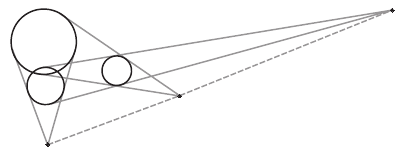
\includegraphics[scale=1]{pics/3circs}
\caption{Три окружности и их фокусы.}
\label{pic:3circ}
\end{figure}

\parit{Примечания.}
В моей предыдущей книге \cite{59} предлагается построить три сферы с экваторами на данных окружностях, а затем рассмотреть плоскость, касающуюся этих трёх сфер.
Однако Джером Льюис, профессор информатики в Университете Южной Каролины в Апстейте, справедливо указал мне на то, что такой плоскости может не быть!
Например, её нет, когда две окружности большие, и между ними находится меньшая.

Однако доказательство можно спасти, не отказываясь от основной идеи.
Попробуйте найти способ.

\medskip

Следующая задача является отличным представителем головоломок про знания о знаниях.

\subsection*{Самоубийцы Точкинска}\rindex{Самоубийцы Точкинска}

У каждого жителя Точкинска есть красная или синяя точка на лбу.
Если он когда-либо решит, что знает, какого цвета его точка, то покончит с собой.
Все точкинцы встречаются каждый день и видят друг друга.
Однажды приезжий сказал им что-то (что угодно не тривиальное) о числе синих точек.
Докажите, что рано или поздно все точкинцы покончат с собой.

\parit{Примечания.} Что-то \emph{нетривиальное} означает, что некоторое число синих точек делает это утверждение верным, а какое-то другое число --- неверным.
Однако мы не предполагаем, что то, что сказал им приезжий, является правдой!
Увы, точкинцы легковерны --- они верят всему, что слышат, если только их собственные глаза не говорят обратное.

\medskip

Возможно, вы помните задачу об инфекции на шахматной доске --- прекрасную головоломку, в которой надо доказать, что нельзя заразить доску размера $n \times n$, начиная с менее чем $n$ заражённых клеток;
клетка заражается, если две или более из её соседей (по сторонам) заражены.
Показать, что $n$ заражённых клеток достаточно, было лёгкой частью; достаточно заразить клетки на главной диагонале.

А что случится, если увеличить размерность?

\subsection*{Заражённые кубы}\rindex{Заражённые кубы}

Инфекция распространяется по $n^d$ единичным $d$-мерным кубам в кубе $n \times n \times \dots \times n$ следующим образом: если у единичного куба $d$ или более заражённых соседей, то он сам заражается.
(Соседями считаются кубы с общей гипергранью; в частности, у куба не может быть более $2d$ соседей.)

Докажите, что \emph{можно} заразить все кубы, начав с $n^{d-1}$ заражённых кубов.

\medskip

Задачи, в которых заключённые надевают красные или синие шляпы, затем видят цвета шляп своих товарищей по несчастью и должны угадать свой собственный, произвели довольно много шума.
В версии, ставшей темой статьи в Нью-Йорк таймс \cite{50}, каждый заключённый мог выбрать, угадывать ли или нет.
При этом все заключённые будут казнены, за исключением случая, когда все угадывающие правы и при этом нашёлся хотя бы один угадывающий.
Как обычно, заключённым было разрешено сговориться заранее, но всякое общение прекращалось, как только они увидели шляпы.

Конечно же один заключённый может угадывать, а все остальные молчать --- 
это обеспечит 50\%-ю вероятность выживания. 
Может показаться, что лучшего добиться нельзя.
Однако есть гораздо лучшая стратегия --- $n$ заключённых смогут добиться того, чтобы вероятность казни была бы примерно $1/n$.

Для тех, кто считает такие задачи чересчур фантастичными, приготовьтесь:
следующий вариант заставит вас думать, что старые версии слишком реалистичны.

\subsection*{Шляпы и бесконечность}\rindex{Шляпы и бесконечность}\label{Шляпы и бесконечность}

Каждому из бесконечного множества заключённых, пронумерованных $1,2,\dots$, должна быть надета красная или синяя шляпа.
По заранее договорённому сигналу все заключённые являются друг перед другом, так что каждый видит цвета всех шляп.
При этом никакое общение не позволяется.
Затем каждого заключённого отводят в сторону и спрашивают, какого цвета его шляпа.

Если ошиблось бесконечное число заключённых, то \emph{всех} казнят. 
У заключённых есть шанс сговориться заранее;
существует ли стратегия, которая обеспечит их выживание?

\parit{Примечания.}
Обратите внимание, что это более простая задача, чем описанная выше:
здесь нельзя молчать, нет никаких параметров и нет вероятности;
от вас требуется чистое решение.
Однако необходимо предположить, что каждый заключённый способен воспринять всю последовательность цветов шляп, которую он видит, и каким-то образом обработать всю эту информацию за конечное время, прежде чем высказать свою догадку.

\subsection*{Все правы или все неправы}\rindex{Все правы или все неправы}

На этот раз обстоятельства те же самые, но цель другая:
угадывания должны быть либо \emph{все верными}, либо \emph{все неверными}.
Существует ли выигрышная стратегия?

\parit{Примечания.}
Конечная версия этой задачи довольно лёгкая:
заключённые могут, например, заранее решить, что каждый будет угадывать цвет своей шляпы, предполагая, что общее число красных шляп чётно.
Если это на самом деле так, то все окажутся правы;
в противном случае все неправы.
Однако, если число красных шляп бесконечно, как определить, чётно ли их число?

\medskip

Вернёмся к конечному числу заключённых, но с числами вместо шляп.

\subsection*{Цифры на лбах}\rindex{Цифры на лбах}

На этот раз на лбу каждого из 10 заключённых написана цифра от 0 до 9 (например, все могут быть двойками).
В установленное время каждый будет выставлен перед всеми остальными, затем отведён в сторону и его попросят угадать свою собственную цифру.

Для того чтобы избежать общей казни, хотя бы один из заключённых должен угадать правильно.
Как обычно, у заключённых есть возможность сговориться заранее.
Найдите для них стратегию, обеспечивающую выживание.

\subsection*{Заключённый дальтоник}\rindex{Заключённый дальтоник}

Заключённые из предыдущей головоломки вдруг узнают, что к сожалению у одного из них (у Шрека) зелёная кожа,
а цифры будут написаны красным.
При этом один из заключённых (Майкл) страдает дальтонизмом, то есть не различает красное и зелёное.
Поэтому Майклу придётся делать свои предположения только исходя из 8 видимых ему цифр.
Остальные заключённые, включая Шрека, по-прежнему смогут видеть все 9 цифр, кроме своей собственной.
Требуется доказать, что заключённые теперь уже не смогут гарантированно избежать казни.

\medskip

В последней задаче про заключённых, числа встречаются со шляпами. 

\subsection*{Числа со шляпами}\rindex{Числа со шляпами}

На лбу каждого из $n$ заключённых написаны различные вещественные числа, так что каждый может видеть числа остальных, но не своё собственное.
Как обычно, после просмотра никакого общения не допускается, но затем каждый заключённый должен независимо выбрать себе шляпу --- либо красную, либо синюю.

Цель состоит в том, чтобы цвета шляп чередовались в порядке, определённом числами.

Как игроки, которым разрешено сговариваться заранее, могут максимизировать вероятность успеха?

\medskip

Мы завершаем наши визиты к старым головоломкам одной, которая берёт своё начало по крайней мере с середины девятнадцатого века, но не была решена до 2006 года.
Мы не будем просить вас доказывать правильность вашего решения (хотя, конечно, вы можете попробовать) --- для разгадки этой головоломки потребовалось пять профессиональных математиков, и даже сейчас ответ известен только с точностью до постоянного множителя.
Однако угадывание конструкции --- отличная проверка вашей интуиции.

\subsection*{Кирпичная стенка}\rindex{Кирпичная стенка}\label{Кирпичная стенка}

На какое расстояние стенка из $n$ кирпичей может зайти за край стола?

\parit{Примечания.} Можно предположить, что кирпичи --- однородные прямоугольные твёрдые тела длины 1 без трения;
их ставят горизонтально в общей вертикальной плоскости.
Однако не нужно предполагать, что на каждом уровне только один кирпич.

\section*{Источники и решения}

\subsubsection*{Трое аборигенов на перекрёстке}

Этот вариант задачи про логика и аборигенов пришёл ко мне от двух матфизиков, Владаса Сидоравичюса и Сени Шлосмана.
Кажется, что случайный абориген спутает все карты, однако решение есть.

Сначала надо позаботиться о том, чтобы \emph{второй} спрошенный абориген не был из случайного племени.
Это необходимо, ведь за первый вопрос дорогу не узнать, а если второй абориген случайный, то мы вовсе ничего не узнаем.

С другой стороны, этого достаточно, ведь далее можно использовать вопрос с обычным вывертом, типа «А если бы я спросил вас, ведёт ли первая дорога к деревне, вы бы сказали „да“?»

Чтобы достичь этой цели, вам нужно будет задать аборигену А что-то об аборигенах Б или В, а затем использовать ответ, чтобы выбрать между Б и В.
Вот рабочий вариант: «Верно ли, что Б ответит правду с большей вероятностью чем В?»

Забавно, что если А ответит «да», то надо спрашивать у В, а если «нет», то у Б!
Ведь если А говорит правду, вы хотите обратиться к тому, кто \emph{меньше} всего склонен говорить правду, то есть к лжецу.
Если же А лжец, то вам нужен \emph{более} правдивый из его спутников, а именно правдолюб.
Конечно же, если А --- случайный, то нет разницы, кого выбрать.

В колонках Мартина Гарднера отмечалось, что в первоначальной задаче с одним аборигеном логик может дойти до деревни даже если забыл, какое из слов на местном языке (предположительно «пиш» и «туш») означает «да» и «нет».
Если желаете развлечься, попытайтесь аналогично изменить вышеуказанный протокол.

Если случайный абориген выбирает из «да» или «нет», подбрасывая монету в уме, то, конечно же, \emph{одного} вопроса недостаточно.
Однако, если предположить, что он заранее случайно выбирает между правдой и ложью, а затем отвечает логически,
то для этого случая Анупам Джайн из Университета Южной Калифорнии придумал следующий вопрос:
\begin{itemize}
 \item[] \emph{Если я выберу из двух ваших спутников того, чей ответ с наименьшей вероятностью будет совпадать с вашим, и спрошу его, ведёт ли первая дорога в деревню, ответит ли он „да“?}
\end{itemize}
Утверждается, что если ответ «нет», то первая дорога --- правильная, в противном случае --- вторая.

Ключевой случай, когда этот вопрос задаётся случайному отвечающему.
Если случайный абориген решит солгать, то ответ правдолюба на вопрос будет наименее вероятно совпадать с его ответом.
Правдолюб скажет «да», и так как случайный отвечающий решил солгать, он скажет противоположное и, таким образом, ответит «нет».

Если случайный отвечающий решил сказать правду, то ответ правдолюба будет наименее вероятно совпадать с его ответом.
Лжец скажет «нет», и так как случайный отвечающий решил сказать правду, он опять скажет «нет».

Если логик обращается к правдолюбу, то ответ лжеца наименее вероятно совпадёт с его ответом,
и он скажет то, что сказал бы лжец: «нет».

Точно так же, если вторая дорога правильная, все ответы будут «да».

\subsubsection*{Новая встреча с тремя окружностями}

Эту задачу иногда называют «окружностями Монжа».

На сайте Cut-the-knot следующее доказательство приписывается Натану Боулеру из Тринити-колледжа в Кембридже.
Оно использует конусы, построенные на окружностях вместо сфер.
Обозначим их через $C_1$, $C_2$ и $C_3$; мы предполагаем, что это прямые конусы, то есть с углом 90° при вершине.
(На самом деле, достаточно, чтобы углы при их вершинах были одинаковы.)
Каждая пара конусов определяет две (внешние) касательные плоскости, скажем, $P_1$ и $Q_1$ (для конусов $C_2$ и $C_3$), $P_2$ и $Q_2$ (для конусов $C_1$ и $C_3$), и, наконец, $P_3$ и $Q_3$ (для конусов $C_1$ и $C_2$).

Каждая пара плоскостей $P_i$, $Q_i$ пересекается по прямой $L_i$, которая проходит через вершины касаемых конусов, а также через точку, где соответствующие касательные пересекаются.
Таким образом, прямые $L_1$ и $L_2$ проходят через вершину $C_3$,
прямые $L_1$ и $L_3$ через вершину $C_2$,
а $L_2$ и $L_3$ через вершину $C_1$.
Следовательно, эти три прямые копланарны (все они лежат на одной плоскости, определённой тремя вершинами конусов); пересечение этой плоскости с исходной плоскостью окружностей и есть та самая прямая через три фокуса --- победа!

\subsubsection*{Самоубийцы Точкинска}

Эта головоломка про знания о знаниях удивляет своей общностью.
Она досталась мне от Ника Рейнголда из AT\&T Labs.
Различные частные случаи (иногда с ужасными формулировками%
\footnote{Есть вариант про казни неверных жён.\pr}%
) известны на протяжении многих десятилетий.
Многим из вас наверняка известен вариант, когда у всех точки синие, а приезжий сказал: «Есть хотя бы одна синяя точка».

То есть, что им не скажешь --- будет катастрофа, 
это впечатляет.
Но, ещё удивительней, что все обречены даже \emph{если каждый видит, что приезжий соврал}. 
Мы это скоро докажем, но сначала рассмотрим простой частный случай, показывающий как это работает.

Предположим, что в Точкинске живут всего три жителя, и у всех на лбу синие точки,
а приезжий сказал им, что все точки красные.
Конечно же все видят, что это не так.
Однако первый из них думает следующее: предположим, что моя точка красная; тогда второй житель видит мою красную точку и задаётся вопросом, видит ли третий житель две красные точки?

«Если да» --- думает второй, --- «то третий житель поверит приезжему и совершит самоубийство этой же ночью, несмотря на то, что у него точка синяя».

Если же этого не произошло, то второй житель правильно заключит, что третий увидел только одну красную точку, и совершит самоубийство во вторую ночь.
Поскольку ни одно из этих событий не происходит, первый житель заключает, что второй не увидел красной точки.
Он заключает, что его точка синяя и прощается с жизнью на третью ночь.

Для доказательства общего случая введём некоторые обозначения.
Пусть $S\subset\{0,1,\dots,n\}$ --- множество чисел $x$ с таким свойством: \emph{если у $n$ точкинцев $x$ синих точек, то утверждение приезжего верно}.
По предположению, $S$ --- собственное подмножество; то есть $S$ и его дополнение непусты.
Пусть $b$ --- число синих точек на самом деле;
$b$ может принадлежать $S$, а может и не принадлежать.

Обозначим через $B_i$ множество возможных чисел синих точек, с точки зрения $i$-того точкинца.
Если $b_i$ --- число синих точек, которое он видит на других, то до заявления приезжего, $B_i=\{b_i,b_i\z+1\}$.

Если в какой-то момент $B_i$ сокращается до одного значения, то $i$-й точкинец обречён.
Это произойдёт в первую же ночь в случае, если  $|B_i\z\cap S|=1$, но это произойдёт и на следующую ночь после любого самоубийства.
Действительно, все точкинцы с одинаковым цветом точек ведут себя одинаково, ведь они все видят одинаковое число точек каждого цвета.
Таким образом, если какой-то точкинец видит, что кто-то совершил самоубийство, то (справедливо) считает, что цвет точки этого человека отличается от его собственного. 
Следовательно, он знает свой собственный цвет и обречён.

Для заданных $S$ и $b$, обозначим через $d(b)$ число шагов (увеличений или уменьшений на $1$), необходимое для того, чтобы попасть из $b$ за пределы $S$ или внутрь $S$.
Другими словами, $d(b)$ это наименьшее $k$, такое что $b+k$ или $b-k$ находится в $\{0, 1, \dots, n\}$, но не в $S$ (если $b$ не в  $S$) или в $S$ (если $b$ в $S$).

Например, если $n=10$ и 
$S=\{0,1,2,9,10\}$, то 
$d(0)=3$, 
$d(1)=2$, 
$d(2)=d(3)=1$, 
$d(4)=2$, 
$d(5)=d(6)=3$, 
$d(7)=2$, 
$d(8)=d(9)=1$ и
$d(10)=2$.

Как уже отмечалось, если $d(b)=1$, то самоубийства произойдут уже в первую ночь.
Теперь сделаем более общее утверждение: \emph{первые самоубийства произойдут именно в $d(b)$-ю ночь}.

Доказательство ведётся индукцией по $d(b)$.
Предположим, что это верно при $d(b)<t$, а теперь пусть $d(b)=t>1$.
После $(t-1)$-й ночи, поскольку самоубийств ещё не было, все знают, что $d(b)\ge t$.
Однако, если $d(b)=t$, то $d(b-1)$ либо $d(b+1)$ равно $t-1$.
В первом случае синеточкенцы, которые знают, что синих точек $b$ (то, что на самом деле) или $b-1$, 
могут исключить случай $b-1$, и им конец.
Во втором случае красноточкенцы могут исключить $b+1$, и им придётся покончить с собой.
Наконец, если $d(b-1)\z=d(b+1)=t-1$, то никто не переживёт эту ночь.

Поскольку $d(b)$ не превышает $n$, к $n$-й ночи все погибнут.
Также можно увидеть, что они продержатся столько времени только в четырёх крайних случаях:
если $b=0$ и $S=\{n\}$ или $\{0,1,\dots,n-1\}$,
а также если $b=n$ и $S=\{0\}$ или $\{1,2,\dots,n\}$.
Иначе говоря, время выживания максимально если приезжий либо делает наименее информативное верное заявление,
либо высказывает самую безумную ложь.
Также стоит отметить, что определение $d(b)$ не различает 
$S$ и его дополнение --- точкинцы будут вести себя точно так же не зависимо от того скажет ли приезжий «$X$» или «Не $X$».

Можно было бы задаться вопросом, а могут ли точкинцы, зная, что к ним едет кто-то, кто может нарушить явно оправданное правило молчания о цвете точек, организовать какую-то защиту.
Например, все, кто знает, что приезжий соврал, поднимаются и говорят об этом.
К сожалению, немного поразмыслив, можно прийти к выводу, что ни эта, ни какая-либо другая стратегия не спасёт город.

Да, жизнь точкинцев висит на волоске.
Но как ни странно, само это может их и спасти.
Стив Бэббидж, менеджер и криптограф из компании Vodafone, указал на то, что при определённых обстоятельствах некоторые точкинцы смогут пережить вторжение приезжего если подумают, что чьё-то самоубийство было вызвано не знанием цвета, а тем, что тот не выдержал жизни в их смехотворной среде.

\subsubsection*{Заражённые кубы}

То, что изначально \emph{нужно} хотя бы $n^{d-1}$ заражённых единичных кубов (для краткости \emph{участков}), доказывается прямым обобщением двумерного случая, в котором, как мы знаем, периметр заражённой области не увеличивается.
Вместо периметра следует взять $(d\z-1)$-мерную площадь поверхности заражённой области.
Когда новый участок заражается, к этой поверхности добавляется не более чем $d$ его граней,
и в то же время по крайней мере $d$ граней удаляются (те, что отделяют новый участок от заражённых соседей).
Таким образом, площадь поверхности не увеличивается.
В самом конце, она равна площади поверхности большого куба, что составляет $2d \times n^{d-1}$.
Поскольку каждый участок имеет $2d$ граней единичной площади,
начальная площадь поверхности не может превышать $k \times 2d$,
где $k$ --- число изначально заражённых участков.
Отсюда $k\geqslant n^{d-1}$.

Однако на этот раз выбрать начальные $n^{d-1}$ заражённых участков совсем не просто.
Мэтт Кук и Эрик Уинфри из Калтеха нашли способ, который, должен бы сработать, но не смогли это доказать;
их коллега Лен Шульман придумал замечательное доказательство, приведённое ниже (присланное мне Эриком).

Начнём с построения Мэтта и Эрика.
Обозначим участки векторами $(x_1 , x_2 , \dots , x_d )$, где $x_i \in \{1, 2, \dots , n\}$, так что два участка соседствуют, 
если все их координаты кроме одной одинаковы, а по одной различаются на $1$.

Возьмём любое целое число $k$ и заразим все участки, для которых $\sum_i x_i \equiv k\pmod n$.
Эти участки образуют \emph{диагональное подпространство}, оно разбивается на несколько кусков.
Они всё заражают, но странным образом и очень по-разному при разных $k$.
Часто кажется, что просто повезло из-за нескольких совпадений.
Картина сильно отличается от двумерной!

В доказательстве, что это множество подходит, Шульман использовал следующую игру;
в ней сила, препятствующая заражению, передана демону-противнику, который мешает заражающему игроку.
Выберем $k$ и начнём с заражённых участков, описанных выше.

Сначала демон помещает вас на участок $x = (x_1, \dots,x_d )$.
Далее, он выбирает координату $i$.
У вас есть право переместится либо вперёд, либо назад вдоль $i$-й координаты (если $x_i$ равна $1$ или $n$, то выбора нет).
Вы выигрываете, если сможете достичь некоторой точки $x$, из диагонального подпространства $\sum_i x_i \equiv k\pmod n$;
демон выигрывает, если сможет заставить вас бесконечно блуждать.

Утверждается, что если у вас есть стратегия, которая гарантирует победу, то весь большой куб заразится.

Прежде чем доказывать, уточним утверждение: если можно выиграть, начав с $x$, то $x$ заразится.
Действительно, демон может выбрать любое из $d$ направлений,
и победная стратегия срабатывает при каждом выборе.
Это означает, что с вашей стратегией можно победить, начав с любого из $d$ соседей $x$, к которым вы собирались переместиться.
По индукции (по числу шагов до победы), все эти $d$ соседей $x$ заразятся, а значит заразится и $x$.
За базу возьмём случай, с начальным участком $x$ из диагонального подпространства --- в этом случае он уже заражён.

Осталось описать выигрышную стратегию.
Далее последует то, что Шульман называл \emph{алгоритмом телеги}.
Для любого участка $x$ обозначим через $x^*$ значение $-k + \tfrac12 + \sum_i x_i \pmod n$.
Если демон выбрал $i$-ю координату, то следует уменьшить $x_i$ если $x_i > x^*$ (таким образом, $x^*$ также уменьшается, хотя, возможно, и прыгнет с $\tfrac12$ на $n - \tfrac12$).
Если же, $x_i < x^*$, то надо увеличить $x_i$, чтобы значение $x^*$ также увеличилось, или возможно, прыгнуло с $n - \tfrac12$ на $\tfrac12$.
Но стойте --- если вы попали на участок с $x^* = \tfrac12$, то победа ваша!

Отсюда следует, что ход, предписанный алгоритмом, всегда допустим:
нет нужды ходить на участок с $x_i = 0$ или $x_i = n + 1$, до победы.

Теперь мы утверждаем, что демон не может заставить вас зациклиться.
Предположим противное, то есть $x$ циклически повторяется.
Пусть $I$ --- множество индексов, выбранных бесконечное число раз демоном.
Можно считать, что вы уже прошли несколько шагов, и уже ни один индекс, не принадлежащий $I$, больше выбран не будет.
Пусть $y$ будет самым большим значением $x_j$, когда-либо встречавшимся для любого $j \in I$.
Пусть $J$ --- множество индексов в $I$, которые в данный момент имеют это максимальное значение $y$.

Если когда-либо случится, что $x^* > y$, то вы будете увеличивать его на каждом шаге, увеличивая $x^*$, пока он не прыгнет в $\tfrac12$, принеся вам победу.
Следовательно, $x^*$ всегда ниже $y$.
Но тогда, когда демон выбирает $j \in J$, $x_j$ должен уменьшаться до $y - 1$.
В результате $J$ в конечном итоге исчезнет, оставив вас навсегда с меньшим максимальным значением $y$.
А это не может продолжаться вечно --- противоречие.

Отсюда следует, что алгоритм телеги позволяет выигрывать, независимо от того, куда вас высадил демон или как он вас ограничивал.
Существование выигрышной стратегии означает, что заразится весь большой куб --- ура!

\subsubsection*{Шляпы и бесконечность}

Оба ответа --- «Да, стратегия существует» и «Нет, её нет» --- оказываются верными!
Но разве такое возможно?

По моим данным, эта прекрасная загадка была придумана совместно Ювалем Габаем и Майклом О'Коннором (в то время аспирантами Корнельского университета).
Однако решение косвенно содержалось в работе Фреда Гальвина из Канзасского университета.
Кристофер Хардин (Колледж Смита) и Алан Д. Тейлор (Колледж Юнион) затем включили её в статью для American Mathematical Monthly \cite{36}.
Стэн Уэгон предложил её как задачу недели в Маккалестерском колледже.
Дополнительные интересные наблюдения об этой и следующей задаче были сделаны Харви Фридманом (Огайо Стейт), Хендриком Ленстрой (Университет Лейдена) и Джо Булером (Рид Колледж).
Последний из них, а также (независимо) Мэтт Бейкер из Технологического института Джорджии, рассказали мне о ней.
Всё это только небольшая часть истории.
Простите меня, если пропустил ваше имя!

Сначала посмотрим, а что если только конечное число заключённых получат красные шляпы.
Тогда все заключённые это увидят, и если они заранее договорились об этом, все скажут «синий» --- и, конечно же, только конечное число ошибётся.

Та же схема применима, и если только конечное число шляп будут синими или, например, если только конечное число шляп с нечётными номерами будут красными, а конечное число шляп с чётными номерами будут синими.
Можно пойти ещё дальше: если последовательность шляп \emph{периодична} с какого-то места, то все могут угадать цвет, как если бы последовательность была периодичной с самого начала.

Другими словами, последовательность цветов шляп можно считать двоичной записью некоторого вещественного числа $r$ из интервала $[0,1]$, считая (скажем) синий как 1, а красный как 0.
\emph{В конечном итоге периодична} означает, что с какого-то момента некоторое слово из нулей и единиц в ней бесконечно повторяется;
это означает, что $r$ рационально.
Например, последовательность $100101001010101010\dots$, где $01$ бесконечно повторяется, является таким числом; в этом случае число равно дроби $7/12$.
Если бы это произошло, то каждый заключённый с нечётным номером может сказать «синий», а каждый с чётным номером «красный», и все, кроме номеров $3$, $4$, $5$, $6$ и $7$, окажутся правы.

Таким образом, заключённые спасутся, если $r$ рационально.
Однако нет нужды ограничивать стратегию рациональными числами.
Возможно, последовательность будет отличаться лишь в конечном числе мест от двоичного представления $\pi$, в таком случае заключённые могут согласиться угадывать, как если бы шляпы представляли собой точно $\pi$.

На самом деле заключённым надо разделить все возможные последовательности шляп на \emph{классы}, таких, что в каждом классе две последовательности отличаются только в конечном числе мест.
Затем заключённые заранее договариваются о представителе из каждого класса, то есть о каком-то конкретном члене класса.
Если они видят последовательность из этого класса, то каждый угадывает, как если бы фактическая последовательность была равна согласованному представителю.

Более математически, мы говорим, что две последовательности как (скажем) \emph{соседние}, если они отличаются только в конечном числе мест.
Заметим, что
(1) любое $r$ --- сосед самого себя;
(2) если $r$ --- сосед $s$, то $s$ --- сосед $r$; и
(3) если $r$ --- сосед $s$, и $s$ --- сосед $t$, то и $r$ --- сосед $t$.
Это означает, что соседство является тем, что математики называют \emph{отношением эквивалентности}.
Это, в свою очередь, означает, что существует разбиение множества всех последовательностей шляп на классы, так что в каждом классе любые две последовательности являются соседними, а любые две последовательности в разных классах соседями не являются.

Пока всё чисто, но сейчас появится трудность.
Большинство этих классов не будут обладать естественным представителем (как например $\pi$),
а заключённым придётся договориться о представителе в каждом классе.
Утверждение, что это в принципе возможно сделать, называется \emph{аксиомой выбора}.
Если принять аксиому выбора, то заключённые смогут ей воспользоваться, чтобы выбрать по представителю из каждого класса.
Затем, увидав шляпы, заключённые поймут, к какому классу принадлежит последовательность шляп (для этого достаточно смотреть только на шляпы заключённых с более высокими номерами, чем их собственные).
Затем они все угадывают, что их собственный цвет шляпы соответствует тому, что было предсказано согласованным представителем класса, и будет только конечное число ошибок --- дело сделано!

А верна ли аксиома выбора?
Большинство активно работающих математиков предполагают, что да.
Однако известно, что если основные аксиомы с аксиомой выбора образуют не противоречивую систему, то нет противоречия и с отрицанием аксиомы выбора.
Так что так же справедливо предположить, что аксиома выбора не выполняется, как и предположить, что она выполняется.

А если аксиома выбора не выполняется, то заключённые окажутся в трудном положении.
Упомянутые выше Хардин и Тейлор, и независимо Харви Фридман, показали, что со стандартными аксиомами математики у заключённых нет стратегии.
И даже хуже: любая стратегия потерпит неудачу, если только, в определённом смысле, который можно сделать математически точным, заключённые не будут невероятно удачливы.
Так что, если есть опасность стать заключённым, то лучше принять аксиому выбора и взять её с собой.

А вы верите в аксиому выбора?
Подумайте: множество возможных выигрышных стратегий для нашего предполагаемого решения является произведением всех вышеобсуждаемых классов эквивалентности; если нет решения, это означает, что произведение бесконечного числа непустых (да ещё и бесконечных) множеств пусто.
С другой стороны, знаменитый парадокс Банаха --- Тарского говорит, что, используя аксиому выбора, можно разрезать шар на пять частей и собрать из них два шара идентичных исходному!

У меня такое заключение: хотя ни аксиому выбора, ни её отрицание нельзя опровергнуть, любую из них можно сделать смешной.

%\begin{addedbytheeditors}
%\textbf{Редакторам:} Заменил «без аксиомы выбора» на «с её отрицанием», иначе фраза бессмысленна. 
%\end{addedbytheeditors}


\subsubsection*{Все правы или все неправы}

Если вы разобрались с решением предыдущей головоломки (с аксиомой выбора), то здесь не должно быть проблем.
Во первых заключённые соглашаются, как и раньше, на представителя из каждого класса эквивалентности.
Кроме того, они соглашаются, что будут угадывать цвет своих шляп исходя из предположения, что число позиций, в которых последовательность шляп не совпадает с выбранным представителем, чётно.
Как и в случае конечного числа, если это число чётно, то все заключённые будут правы; в противном случае --- все неправы.

Примечательно, что алгебраисты обычно решают эту задачу следующим образом.
Отождествим цвета шляп с множеством $\{0, 1\}$, как и раньше, 
будем думать, что это элементы группы $\mathbb{Z}_2$.
Сумма $\Sigma$ из бесконечного числа копий $\mathbb{Z}_2$ является множеством всех последовательностей состоящих из нулей и единиц, в которых только конечное число единиц (синие шляпы).
Существует естественный гомоморфизм (отображение) из $\Sigma$ в $\mathbb{Z}_2$, который даёт 0, если число единиц чётно, и 1, если нечётно.
Стандартная теорема о расширении позволяет нам расширить этот гомоморфизм на произведение $\mathbb{Z}_2$, которое является множеством всех последовательностей $\{0, 1\}$.
Затем заключённые соглашаются угадывать, предполагая, что значение этого гомоморфизма равно (скажем) 0.

Конечно, в \emph{доказательстве} теоремы о расширении нужна аксиома выбора, поэтому это доказательство на самом деле ничем не отличается от других.

Означает ли это, что для версии с «все правы» или «все неправы» бесконечной задачи о шляпах также требуется аксиома выбора?
Я так думал, пока Тина Кэрролл (студентка-математик в Технологическом институте Джорджии) не показала мне решение, которое \emph{гораздо} проще и не требует аксиомы выбора или какой-либо математики вообще.

Каждый говорит «зелёный»!!

\begin{addedbytheeditors}
Про гомоморфизм $\mathbb{Z}_2^\infty\to \mathbb{Z}_2$ можно думать, как про обобщённую сумму бесконечной последовательности элементов из $\mathbb{Z}_2$.
Поэтому второе решение --- это по сути спасение рассуждения с чётностью числа красных шляп, прекрасно работающего в конечном варианте задачи.
Про этот гомеоморфизм можно думать уймой способов, например как об ультрапределе суммы первых $n$ членов последовательности по неглавному ультрафильтру.
Можно действовать и более геометрически, через выбор точки в чех-стоуновской компактификации натуральных чисел.\pr
\end{addedbytheeditors}


\subsubsection*{Цифры на лбах}

Эта головоломка пришла ко мне независимо от нескольких людей, включая Ногу Алона из Тель-Авивского университета.
Сам Нога многократно показывал, что во многих задачах бывает полезно ввести вероятность, даже если в формулировке её нет.
В нашей задаче, если предположить, что числа, написанные на лбах, выбираются независимо и равномерно случайным образом, то каждый заключённый угадает правильно с вероятностью $\tfrac1n$, независимо от того, что он скажет.

Положим, что заключённые пронумерованы от $0$ до $n-1$.
Мы хотим, чтобы вероятность того, что какой-то заключённый угадает правильно, была равна $1$.
Значит нам нужно, чтобы $n$ событий типа \emph{«$k$-й заключённый угадывал правильно»} были бы взаимоисключающими.
Другими словами, ни одно из них не может произойти одновременно с другим.
В противном случае вероятность хотя бы одного успешного исхода была бы строго меньше суммы $\tfrac1n + \tfrac1n + \dots + \tfrac1n = 1$.

Для этого следует разделить всевозможные расстановки чисел на $n$ равновероятных сценариев, а затем потребовать чтоб заключённые основывали свою догадку на разных сценариях.
Эта идея подводит к следующему простому решению.
Если $s$ --- сумма чисел на лбах по модулю $n$, то пусть $k$-й заключённый считает, что $s = k$.
Другими словами, он считает, что его собственное число равно $k$ минус сумма оставшихся чисел по модулю~$n$.

В этом случае $s$-й заключенный будет прав (а все остальные нет).

\subsubsection*{Заключённый дальтоник}

Из-за Майкла со Шреком, заключённые не могут реализовать схему из предыдущего решения.
Но это само по себе не означает, что невозможно найти другое решение.

Тем не менее, мы видели, что успешная схема должна предотвратить возможность угадывания правильного числа любыми двумя заключёнными, и это, возможно, подводит Шрека к неприятностям.

Предположим, что \emph{существует} успешная схема; можно считать, что Шрек знает, в точности \emph{что} будет делать Майкл,
ведь он видит каждое число, которое видит Майкл.
Поскольку он видит число Майкла, он может с некоторой вероятностью ($\tfrac1n$) знать, что Майкл угадает правильно.

В этом случае Шрек должен угадать неправильно, но поскольку он не знает своего собственного числа, у него нет возможности это сделать наверняка.
(Выстрелить в воздух, например, назвав $n + 1$, не сработает, ведь тогда сумма вероятностей успеха не достигнет 1.)
Значит заключённые потерпят неудачу с положительной вероятностью.

\subsubsection*{Числа со шляпами}

Эту головоломку мне прислала Николь Имморлика, постдок из Microsoft Research.
Её формулировка (и решение) содержится в статье шести авторов \cite{1}, где она используется в явной конструкции для высокодоходных детерминированных аукционов.

Заключённые могут гарантированно выиграть независимо от распределения чисел.
Прежде чем на лбах появятся числа, они выберут порядок, то есть пронумеруют себя от $1$ до $n$ (скажем, по алфавиту).
Когда все увидят числа, $i$-й заключённый (для каждого $i$) заводит новую нумерацию остальных числами от $1$ до $i - 1$ и от $i + 1$ до $n$, в порядке чисел на их лбах.
Далее он вычисляет, сколько транспозиций старых номеров требуется, чтобы перевести их на место новых номеров.

Предположим, что позже этот $i$-й заключённый узнал своё число, и оказалось, что оно стоит на $j$-м месте после упорядочивания по возрастанию.
Тогда ему придётся сделать ещё $|i - j|$ транспозиций, чтобы завершить перестановку $\sigma$ от всех $n$ старых номеров к $n$ новым номерам.
Действительно, $i$ и $j$ следует поменять местами, а числа между ними нужно сдвинуть вверх или вниз на одну позицию.

Например, предположим, что $n = 4$ и $3$-й заключённый видит на лбах $1$-го, $2$-го и $4$-го числа $2\pi$, $\pi$ и $4\pi$ соответственно.
Тогда он присваивает им новые номера 2, 1 и 4.
Чтобы получить эти номера из старых 1, 2 и 4, надо поменять местами 2 и 1 --- одна транспозиция.
Если он ставит себя на 3-е место, то получает перестановку $1234 \to  2134$.
Его собственное число может быть, скажем, $\pi/2$, и значит он должен был быть первым, а не третьим.
Чтобы получить правильную перестановку  $\sigma  = 1234 \to  3214$, ему надо поменять местами 3 и 1, а затем 2 и 3, то есть нужны ещё две транспозиции.
Конечно же число могло оказаться другим --- мы привели этот последний шаг, чтобы помочь разобраться в последующем  рассуждении.

Допустим, что $\sigma$ --- чётная перестановка, то есть она реализуется чётным числом транспозиций.
Тогда исходная перестановка $i$-го заключённого будет чётной, если $|i - j|$ чётно, и нечётной в противном случае.
Конечно, если $\sigma$ нечётна (как в примере), то справедливо обратное.

Итак, $i$-му заключённому следует выбрать красную шляпу, если он насчитает чётное число транспозиций (в его перестановке остальных $n - 1$ чисел) и его собственный старый номер $i$ чётен, или же если он насчитает нечётное число транспозиций, и $i$ нечётно.
В противном случае он выбирает синюю.
В приведённом примере $i$ нечётно, и $3$-й заключённый сделал нечётное число (одну) транспозицию, поэтому он выберет красную шляпу.

Если перестановка $\sigma$ оказалась чётной, то этот выбор означает, что заключённый $i$ будет выбирать красную шляпу только тогда, когда $i$ и $|i - j|$ оба чётны или когда $i$ и $|i - j|$ оба нечётны --- другими словами, когда $j$ чётно.
Таким образом, в новом порядке каждый заключённый с чётным номером будет носить красную шляпу, а каждый с нечётным --- синюю.

Если же $\sigma$ нечётна (как в примере), то в новом порядке красные шляпы будут надеты на заключённых с нечётными номерами, и в любом случае они победили.

\subsubsection*{Кирпичная стенка}

Вопрос как уложить $n$ кирпичей, максимизируя выступ за край стола, был явно поставлен в 1923 году Дж. Г. Коффином \cite{12}.
Однако другие формулировки известны с 1850 года.
Благодаря Мартину Гарднеру этот вопрос стал очень известным, его используют по всему миру при знакомстве с гармоническим рядом.

Забавно, но несмотря на широко распространённое мнение об обратном, знаменитая \emph{гармоническая стопка} (см. рис. \ref{pic:kirpich1}) далека от оптимального решения, если только, как иногда бывает, головоломка представлена с ограничением одного кирпича на уровень.
Более того, часто отмечается, что до начала постройки надо решить, 
какого выступа мы хотим добиться --- это тоже неверно.

\begin{figure}[ht!]
\centering
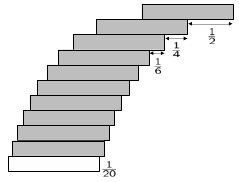
\includegraphics[scale=1]{pics/kirpich1}
\caption{Десятикирпичная гармоническая стопка.}
\label{pic:kirpich1}
\end{figure}

Чтобы получить гармоническую башню, заметим что верхний кирпич не может выступать за  кирпич под ним больше, чем на $1/2$ (при единичной длине кирпича).
В этом случае центр тяжести двух верхних кирпичей находится на $1/4$ левее края нижнего кирпича, поэтому второй сверху кирпич не может выступать за следующим под ним, больше, чем на $1/4$.
Продолжая таким образом, $k$-й сверху кирпич, выступает на $\tfrac1{2k}$ над $(k + 1)$-ым, а значит общий выступ составит 
\[\tfrac12+\tfrac14+\dots+\tfrac1{2k}=\tfrac12(1+\tfrac12+\dots+\tfrac1k)=H_n/2,\]
где $H_n$ --- $n$-я частичная сумма гармонического ряда, она растёт как натуральный логарифм~$n$.

Поскольку гармонический ряд расходится, можно прийти к (правильному) выводу, что если кирпичей достаточно, то можно добиться произвольно большого выступа.
Если строить башню таким образом, то придётся решить заранее, какой выступ нам нужен --- он ограничивается положением самого нижнего кирпича.

\begin{figure}[htb!]
\centering
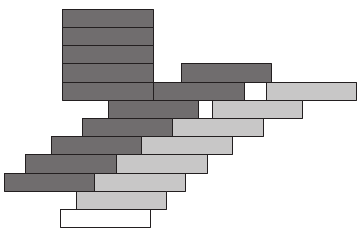
\includegraphics[scale=1]{pics/kirpich2}
\caption{Максимальный выступ для 19-и кирпичей.}
\label{pic:kirpich2}
\end{figure}

Однако, как часто отмечается, можно добиться большего, если использовать несколько кирпичей как противовес другим.
Уже в декабре 2005 года, Дж. Ф. Холл \cite{35} отметил, что общий выступ можно увеличить примерно вдвое (то есть, сделать его около $\ln n$) используя стопку кирпичей, в которой каждый выступает над предыдущим, и противовесом к ним служат дополнительные кирпичи. %??? она не ``cover article''
На самом деле, вплоть до 19 кирпичей такие стенки дают максимальный выступ; см. рис. \ref{pic:kirpich2} для случая $n = 19$.
Однако Холл неверно заключил, что его стенки (называемые хребетными за из-за того, что кирпичи, поддерживающие самый крайний кирпич, образуют стопку с одним кирпичом на уровень) оптимальны в общем случае.

\begin{figure}[htb!]
\centering
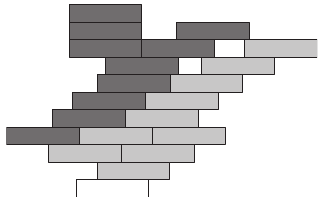
\includegraphics[scale=1]{pics/kirpich3}
\caption{Максимальный выступ для 20-и кирпичей.}
\label{pic:kirpich3}
\end{figure}

\begin{figure}[htb!]
\centering
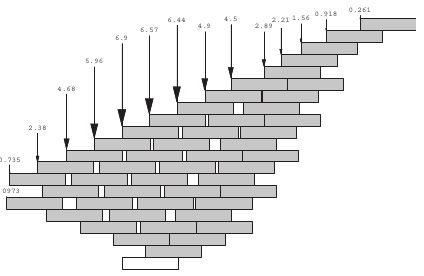
\includegraphics[scale=1]{pics/kirpich4}
\caption{Максимальный выступ для 100 кирпичей.}
\label{pic:kirpich4}
\end{figure}

\begin{figure}[htb!]
\centering
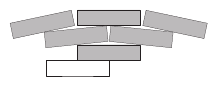
\includegraphics[scale=1]{pics/kirpich5}
\caption{Перевёрнутый треугольник разваливается начиная с трёх слоёв.}
\label{pic:kirpich5}
\end{figure}

Важный шаг сделали Майк Патерсон и Ури Звик в своей статье \cite{47} (она появилась в январе 2006 года, то есть написана до публикации статьи Холла).
Они доказали, что Холл правильно вычислил возможный выступ хребетных стенок.
Однако они также показали, что хребетные стенки перестают быть оптимальными начиная с 20 кирпичей.
Что ещё поразительней, они построили стенку, дающую \emph{экспоненциально лучший} выступ, чем то, что считалось возможным.

Наилучшая стенка из 20 кирпичей изображена на рис. \ref{pic:kirpich3};
она лишь незначительно обгоняет хребетную стенку Холла.
Однако, как видно из рис. \ref{pic:kirpich4},  при больших $n$ лучшие конфигурации перестают напоминать хребетные.
Стрелки в верхней части рис. \ref{pic:kirpich4} обозначают дополнительный вес некоторых не показанных кирпичей (из разрешённых 100), их положения определены неоднозначно.

На самом деле, для очень больших значений $n$ лучший выступ достигается для стенок, как будто вырезанных из обычной кирпичной кладки --- середина кирпича располагается ровно над стыком пары кирпичей ниже.
Тем не менее наиболее очевидные такие стенки разваливаются.
В книге Джаргодзки и Поттера \cite{38} (рекомендуется, несмотря на следующую ошибку) утверждалось, что устойчивы перевёрнутые треугольники (один кирпич внизу, затем два, затем три и так далее), но на самом деле они разваливаются начиная с трёх слоёв (см. рис.~\ref{pic:kirpich5}).  

Ромбы (с добавлением кирпича на слой, до определённого момента, а потом назад до одного) устойчивы до семи слоёв, и на рис. \ref{pic:kirpich6} показано, что происходит далее.

\begin{figure}[htb!]
\centering
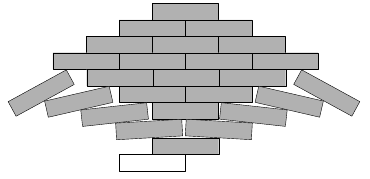
\includegraphics[scale=1]{pics/kirpich6}
\caption{Девятислойный ромб разваливается.}
\label{pic:kirpich6}
\end{figure}

Вместо этого Патерсон и Звик построили стены, приблизительно параболической формы, показанные на рис. \ref{pic:kirpich7}.
Они строятся (и их устойчивость доказывается) рекурсивно, складывая то, что они называют $k$-плитами для последовательно возрастающих $k$.
Одна $k$-плита состоит из $2k + 1$ чередующихся слоёв, в каждом из которых по $k + 1$ и $k$ кирпичей.
Выступ, достигнутый параболической стеной из $n$ кирпичей, имеет порядок $\sqrt[3]{n}$ (кубический корень).%
\footnote{Мы говорим, что функция $f (n)$ (в нашем случае максимальный выступ для $n$ кирпичей) имеет порядок $g(n)$ если существуют положительные константы $c$ и $c'$ такие, что $cg(n) < f (n) < c' g(n)$.}

\begin{figure}[htb!]
\centering
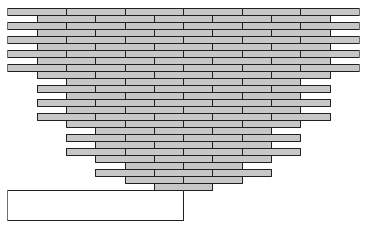
\includegraphics[scale=1]{pics/kirpich7}
\caption{Параболическая стена.}
\label{pic:kirpich7}
\end{figure}

А можно ли это улучшить?
Ромбы или перевёрнутые треугольники, если бы они не разваливались, давали бы асимптотически лучший выступ, порядка $\sqrt{n}$ (квадратный корень).
Однако совсем недавно Патерсон и Звик вместе с Ювалем Пересом, Миккелем Торупом и автором этих строк \cite{48} смогли показать, что порядок $n^{1/3}$ оптимален.

\begin{figure}[htb!]
\centering
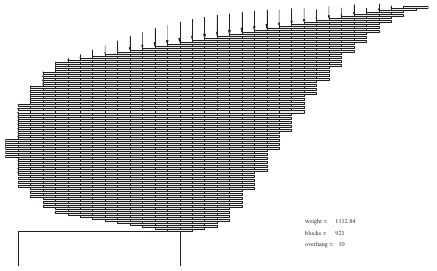
\includegraphics[scale=1]{pics/kirpich8}
\caption{Эта лампоподобная форма стены возможно оптимальна.}
\label{pic:kirpich8}
\end{figure}

И всё же это не означает что параболические кирпичные стены лучше всех.
Они дают выступ примерно $\tfrac3{16}n^{1/3}$, a другие могут дать $cn^{1/3}$ для большей константы $c$.
Патерсон и Звик считают, что лучшая форма для больших $n$ --- это форма «масляной лампы» на рис. \ref{pic:kirpich8}.

\begin{figure}[htb!]
\centering
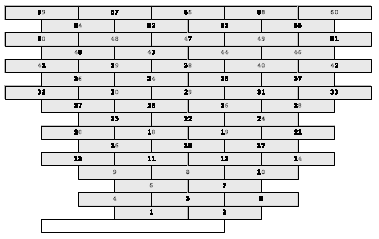
\includegraphics[scale=1]{pics/kirpich9}
\caption{Стенка, строящаяся кирпич за кирпичом.}
\label{pic:kirpich9}
\end{figure}

Параболическую кирпичную стену нельзя построить кирпич за кирпичом.
Причина в том, что, как и все устойчивые конфигурации, показанные выше, она находится на грани устойчивости.
Однако, немного изменив параболу, её всё же можно построить кирпич за кирпичом.
На рис. \ref{pic:kirpich9} показана такая модификация, все ещё обеспечивающая выступ порядка $n^{1/3}$.

Конечно же, стоит помнить, что настоящие кирпичи не идеально прямоугольны и ещё могут ломаться.
Поэтому не пытайтесь это делать дома.

\begin{addedbytheeditors}
\textbf{Редакторам.}
У меня аллергия на эту задачу --- думаю, что здесь очень много ляпов. Пожалуйста, проверьте аккуратно.
\end{addedbytheeditors}

\chapter{Серьёзные испытания}


\setlength{\epigraphwidth}{.80\textwidth}
\epigraph{Со временем разум поднимется на более высокий уровень знаний, но никогда не поймёт как он там оказался.
%There comes a time when the mind takes a higher plane of knowledge but can never prove how it got there.
}{--- Альберт Эйнштейн (1879---1955)}

Ну да, как будто бы предыдущие головоломки не были сложными, а тут ещё несколько непростых задач.
Хотя, может случиться, что некоторые из них покажутся попроще.
Ведь то, что ставит одного в тупик, бывает легко другому.


\subsection*{Торт-мороженое}\label{Торт-мороженое}

На столе стоит цилиндрический торт-мороженое сверху покрытый шоколадной глазурью.
Мы последовательно отрезаем от него дольки с углом $x$, где $x$ произвольно,
каждый раз долька переворачивается и вставляется обратно в торт
(рис. \ref{pic:tort}).

Докажите, что после конечного числа таких операций вся глазурь снова окажется сверху!


\begin{figure}[htb!]
\centering
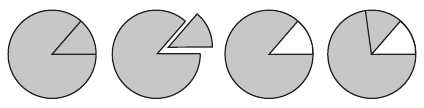
\includegraphics[scale=1]{pics/tort}
\caption{Разрез, переворот, и снова разрез.}
\label{pic:tort}
\end{figure}

\parit{Примечание.}
Я называю такие задачи \emph{вроде неверно расслышанные}.
Да-да, угол $x$ может быть иррациональным, в этом случае вы никогда не отрежете одинаковый кусок дважды.
Придётся отрезать довольно много долек, но всё же конечное число.
К счастью, торт-мороженое самовосстанавливаются.

\subsection*{Прыгание и перепрыгивание}

Лягушка прыгает по длинной цепочке кувшинок;
на каждой кувшинке она подбрасывает монету, чтобы решить, прыгнуть ей на два вперёд или на один назад.
На какой доле кувшинок она побывает?

\subsection*{Три тени кривой}\label{Три тени кривой}

Существует ли простая замкнутая кривая в трёхмерном пространстве, все три проекции которой на координатные плоскости являются деревьями?

\parit{Примечание.}
Это означает, что тени кривой, в трёх координатных направлениях, не содержат циклов.
На рис. \ref{pic:proj1} изображена кривая, которая почти подходит: две её тени являются деревьями, но третья содержит (и даже является) циклом.

\begin{figure}[htb!]
\centering
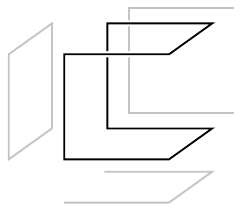
\includegraphics[scale=1]{pics/proj1}
\caption{Замкнутая кривая у которой пара проекций деревья.}
\label{pic:proj1}
\end{figure}

\subsection*{Игроки и победители}

Тристану и Изольде предстоит очутиться в ситуации с очень ограниченной связью, в которой Тристан будет знать, какие две из 16 баскетбольных команд сыграли матч, а Изольда узнает, кто выиграл.
Сколько битов необходимо передать им друг другу, чтобы Тристан узнал, кто одержал победу?

\parit{Примечание.}
Эта задача по \emph{коммуникационной сложности}.
Если бы Изольда знала, кто играл, а также кто выиграл, она могла бы отправить один бит, чтобы сообщить Тристану, выиграла ли (скажем) команда, идущая первой по алфавиту.
Без этой информации она могла бы просто отправить четыре бита, чтобы определить победившую команду.
А можно ли обойтись меньшим числом битов?

\medskip

И снова задача по коммуникационной сложности, но посложней.

\subsection*{Подсказка для Чарли}

Алиса и Боб знают да-нет ответы на все $n$ вопросов экзамена, который сдаёт Чарли.
Чарли нужен только ответ на $k$-й вопрос, но ни Алиса, ни Боб не знают значение $k$.
Вместо этого Алиса знает число $i$, Боб --- число $j$, такие, что $k = i + j \pmod n$.
При этом Чарли знает оба числа $i$ и $j$.

Если бы Алиса не могла передать никакой информации,
то Бобу пришлось бы отправить Чарли все ответы (всего $n$ битов), чтобы Чарли смог узнать нужный ему ответ.

Докажите, что если Чарли получит всего один бит от Алисы, то Бобу достаточно отправить всего $n/2$ битов.

\subsection*{Сближение по кривой}

\begin{figure}[htb!]
\centering
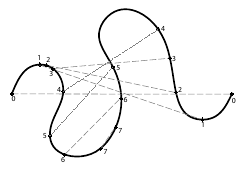
\includegraphics[scale=1]{pics/s-curve}
\caption{Кривая с обоими свойствами.}
\label{pic:s-curv}
\end{figure}

Плоская кривая на рис. \ref{pic:s-curv} обладает следующими свойствами:
(1) расстояние между её конечными точками больше, чем у любой другой пары точек на кривой (мы используем обычное евклидово расстояние на плоскости),
и
(2) взяв по карандашу в обе руки, можно поставить их кончики в концах кривой и двигать их вдоль кривой до встречи, так, чтобы \emph{в процессе расстояние между ними не увеличивалось}.

Существует ли кривая со свойством (1), но без свойства (2)?


\subsection*{Суммы и произведения}

В шляпе лежат все целые числа, большие 1, но меньшие 100.
Из неё достают два числа.
Саманта узнаёт их сумму, а Порфирио --- их произведение.
Далее, Саманта говорит

--- Я знаю, что ты не знаешь этих чисел.

--- Теперь я их знаю --- отвечает Порфирио.

--- Теперь и я знаю --- говорит Саманта.

Что это были за числа?

\begin{figure}[htb!]
\centering
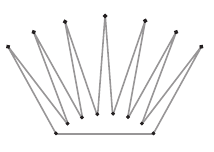
\includegraphics[scale=.95]{pics/korona}
\caption{Корона.}
\label{pic:korona}
\end{figure}

\begin{figure}[htb!]
\centering
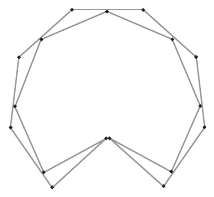
\includegraphics[scale=.95]{pics/wreath}
\caption{Венок.}
\label{pic:wreath}
\end{figure}

\begin{figure}[htb!]
\centering
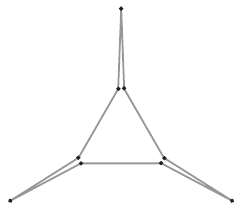
\includegraphics[scale=.95]{pics/treug}
\caption{Схлопнутый треугольник.}
\label{pic:treug}
\end{figure}

\subsection*{Сложенный многоугольник}\label{Сложенный многоугольник}

Какова минимальная площадь простого многоугольника с нечётным числом сторон, каждая из которых имеет единичную длину?

\parit{Примечание.}
Простой многоугольник это замкнутая ломаная без самопересечений, состоящая из конечного числа звеньев.
Многоугольник не обязан быть выпуклым,
например, он может выглядеть как один из многоугольников на рис. \ref{pic:korona},
\ref{pic:wreath} и \ref{pic:treug}.
Очевидно, что у многоугольника на рисунке \ref{pic:treug} площадь не менее площади равностороннего треугольника с единичными сторонами, то есть $\sqrt{3}/4$.
Несложно проверить, что и площадь короны на рис. \ref{pic:korona} ограничена тем же числом.
Но про венок на рис. \ref{pic:wreath} это уже не так очевидно.

Равносторонние \emph{чётно}угольники могут иметь произвольно малую площадь, например, складываясь в очень остроконечную звезду.
Но может нечётноугольники не могут быть меньше $\sqrt{3}/4$ по площади?
Попробуйте это доказать или опровергнуть?


\section*{Источники и решения}

\subsubsection*{Торт-мороженое}

Эта замечательная головоломка досталась мне от французского аспиранта Тьерри Мора,
а тот узнал её от своего школьного учителя Томаса Лаффорга.
Головоломка (происхождения которой Лаффорг точно не знает) на самом деле включала в себя ещё один угол, определяющий зазор между дольками торта.
Даже в этом случае, глазурь ухитрится вернуться наверх после конечного числа операций;
упорные читатели могут в этом убедиться.
Наша формулировка (с нулевым зазором) уже достаточно удивительна и, думается, достаточно сложна.

Если вы решили, что при иррациональном $x$ понадобится бесконечное число операций, то вы совсем не одиноки.
В конце концов, если $n$ операций достаточно, то $n$-й разрез, должен пройти по границе области покрытой глазурью;
как же смогла эта линия оказаться там, где торт никогда не разрезался?

Однако она там окажется.
Причина в том, что когда долька переворачивается, её покрытая и непокрытая области  меняются не только местами, но и порядком.

В этой головоломке, как и во многих алгоритмических задачах, полезно переопределить операцию так, чтобы менялось только состояние (в данном случае, область, покрытая глазурью), а не сама операция, которая пока что у нас меняется на каждом шагу.
В нашем случае достаточно добавить поворот торта после каждой операции так, чтобы разрез всегда приходился на одно и то же место.


\begin{figure}[htb!]
\centering
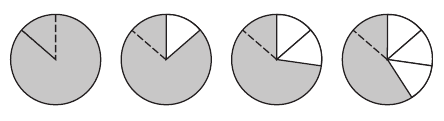
\includegraphics[scale=.9]{pics/tort2}
\caption{Разрезы и перевороты с вращением.}
\label{pic:tort2}
\end{figure}

Будем считать, что $0\degree$ --- направление на север,
$90\degree$ --- на восток и так далее.
Каждый раз будем разрезать по направлениям $0\degree$ и $-x$.
Затем кусок переворачивается через линию $0\degree$ и оказывается между $0\degree$ и $x$.
В это же время остальная часть торта поворачивается по часовой стрелке на угол~$x$.
На рис. \ref{pic:tort2} пунктирные линии показывают где проходят разрезы на первых четырёх шагах.

Чтобы понять дальнейшее рассуждение, проще всего думать, что $x$ чуть больше $360\degree/k$ для некоторого целого $k$.
В этом случае первый разрез по уже отрезанной дольке произойдёт на $k$-м шаге, после того как торт развернётся на полный оборот.

И так, пусть $k$ --- наименьшее число долек, которое надо вырезать, чтобы добраться до конца торта.
Другими словами, $k$ --- наименьшее целое число, большее или равное $360\degree/x$.
Тогда $x \z= y + z$, где $y = 360\degree/k$ и 
\[0\le z <\frac{360\degree}{k-1}-\frac{360\degree}{k}=\frac{360\degree}{(k-1)k}.\]
Конечно же, если $z = 0$, то $x = y = 360\degree/k$, и тогда $k$ операций переведут всю глазурь на дно торта, а ещё $k$ вернут её наверх.
В противном случае, как мы увидим, невозможно достичь момента, когда вся глазурь окажется снизу.

По мере выполнения шагов будут появляться граничные линии (между покрытой и непокрытой областями) под углами $0$, $x$, $2x$, $3x, \z\dots , (k - 1)x$, а затем $x - kz$, $2x - kz$, $3x - kz, \dots , (k - 1)x - kz$,
и затем они повторяются.
Действительно, легко проверить, что описанный набор граничных линий, скажем, $S$, замкнут относительно операции разрез-переворот-поворот.
Одна такая операция переносит $ix$ в $(i + 1)x$, кроме $(k - 1)x$, который переносится в $x - kz$;
она же переносит $ix - kz$ в $(i + 1)x - kz$, кроме $(k - 1)x - kz$, который идёт в $x$.
Тем временем разрез $0\degree$ всё время остаётся на месте.
Отсюда следует, что набор граничных линий всегда является подмножеством $S$.

Уже можно заключить, что конечное число операций вернёт всю глазурь на верх, ведь у нас только $2k - 1$ областей торта между $2k - 1$ линиями из $S$.
Каждая область может быть покрыта или не покрыта глазурью, поэтому число достижимых конфигураций не превышает $2^{2k-1}$.
Значит, процесс зациклится не позднее чем за $2^{2k-1}$ шагов.
Но обязательно ли мы вернёмся к начальной конфигурации (все области покрыты глазурью)?
Да, потому что операция обратима.
Если бы процесс зациклился на другой конфигурации $C$, то существовали бы две разные конфигурации, которые приводили бы к $C$, а это невозможно.

\begin{figure}[hbt!]
\centering
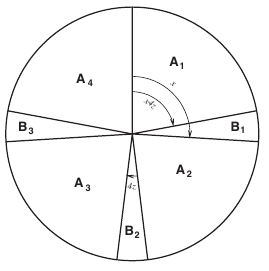
\includegraphics[scale=1]{pics/tort3}
\caption{Области при $x = 93{,}5\degree$ и значит $z = 3{,}5\degree$.}
\label{pic:tort3}
\end{figure}

Однако несложно понять в точности, что и как происходит.
Между граничными линиями в $S$ есть $k$ областей с углом $x - kz$ --- назовём их $A_1$, $A_2, \dots , A_k$, и ещё $k - 1$ область с углом $kz$ --- назовём их $B_1$, $B_2, \dots , B_{k-1}$.
(На рис. \ref{pic:tort3} показан случай $k = 4$ при $x = 93{,}5\degree$.)

С начала процесса, $A$-области становятся не покрытыми глазурью, по порядку.
После $k$ операций они все без глазури.
Затем они снова покрываются глазурью, снова по порядку, до тех пор, пока после $2k$ операций все покроются глазурью.
Тем временем $B$-области также становятся не покрытыми по порядку.
Поскольку их только $k - 1$, после $k - 1$ шагов все они станут не покрытыми, и все снова покроются после $2k - 2$ шагов.

Значит число шагов, необходимых чтобы покрыть глазурью оба типа областей, равно наименьшему общему кратному $2k$ и $2k \z- 2$, то есть $2k(k - 1)$.
Значит потребуется $2k(k - 1)$ шагов, конечно если $x \z\ne 360\degree/k$ ---
в этом случае $B$-области отсутствуют и достаточно $2k$ шагов.

Рассуждая таким же образом, заключаем, что если все области не покрыты глазурью после $n$ шагов,
то $n$ равно нечётному числу домноженному на $k$
и в то же время нечётному числу домноженному на $k - 1$.
Поскольку ровно одно из чисел $k$ и $k - 1$ нечётно, $n$ чётно и нечётно одновременно,
что невозможно.
Значит, если есть $B$-области, то вся глазурь никогда не окажется снизу.

А вот реакция на эту головоломку одного очень известного математика:
«Трудно поверить, что вся глазурь вернётся наверх.
Но если уж это произойдёт, то я уверен, что в какой-то момент вся глазурь окажется снизу!»

\begin{addedbytheeditors}
\textbf{Редакторам:} 
На рис. \ref{pic:tort2} надо добавить отметить отрезок штрихованной линией на первом кружке.
На рис. \ref{pic:tort3} надо поменять $x4z\to x-4z$.
\end{addedbytheeditors}

\subsubsection*{Прыгание и перепрыгивание}

Эту, на вид, простую головоломку придумал Джеймс Б. Ширер --- математик из IBM.
Она появилась на сайте головоломок IBM \cite[апрель 2007]{ponder-this}.
Головоломка вовсе не такая простая, хоть и колется парой полезных приёмов.

Пронумеруем кувшинки по порядку.
Естественно начать с подсчёта вероятности $p$ того, что лягушка, стартуя с $1$, вернётся в какой-то момент в $0$.
Чтобы никогда не возвращаться, ей придётся совершить прыжок вперёд (вероятность $1/2$) и не вернуться обратно трижды (вероятность $1 - p^3$).
Таким образом, $(1 - p) = \tfrac12(1 - p^3)$.
Поделив на $(1 - p)/2$, получим, что $2 = 1 + p + p^2$, а это даёт $p = (\sqrt5 - 1)/2 \z\sim 0{,}618034$ --- знакомое золотое сечение.

Однако подсчитать вероятность того, что лягушка перескакивает конкретную позицию (скажем, $1$), так легко не получается.
Можно было бы начать вычисления с момента, когда лягушка первый раз попадёт в $0$; ведь если это не произошло, то ей придётся попасть в~$1$.
Однако легче вычислить вероятность того, что во время конкретного прыжка лягушка перескакивает через кувшинку, которую она  не посещала и не посетит.

Для того чтобы это произошло, лягушка должна
(а) прыгать вперёд в данный момент,
(б) никогда не возвращаться обратно от того места, где она приземлилась,
и (в) не посещать ту кувшинку, через которую она прыгает, в прошлом.

Можно считать, что кувшинка, которую перепрыгивает лягушка, стоит под номером 0.
Ключ в том, что если развернуть нумерацию и время, то событие (в) становится независимой копией события (б).
Иначе говоря, лягушка ведёт себя ровно так же, если обратить время и рассматривать кувшинки в обратном порядке ---
она равновероятно прыгает на два вперёд или на один назад.
Событие (в) означает, что «достигнув» $-1$, она не «вернётся» в $0$.

Таким образом, вероятность того, что все три события произойдут, составляет $1/2 \cdot (1 - p) \cdot (1 - p) = (1 - p)^2 / 2$.
Однако это ещё не вероятность того, что $0$ пропускается, а только вероятность того, что в данный момент лягушка перепрыгивает через пропущенную кувшинку.

Поскольку лягушка, в среднем, перемещается со скоростью $1/2$, она производит $(1 - p)^2$ пропущенных кувшинок на единицу пройденного пути.
Отсюда следует, что доля кувшинок, на которые она попадает, составляет $1 - (1 - p)^2 \z= (3\sqrt5 - 5) / 2 \sim 0{,}854102$.

\subsubsection*{Три тени кривой}

Эту головоломку мне подбросил Рик Кенион (Университет Британской Колумбии), который увидел её на двери Джорджа Бергмана в Бёркли. 
Бергман услышал её от Хендрика Ленстры из Бёркли и Университета Лейдена.
По словам Бергмана, Ленстра видел игрушку, состоящую из кубической пластиковой коробки с прорезями, образующими своего рода лабиринт на каждой грани.
При этом каждая пара противоположных граней имела одинаковые прорези, так что стержень, перпендикулярный этим двум граням, мог двигаться, проходя через эти два лабиринта.
Но вместо одного стержня был объект, который, по сути, состоял из трёх взаимно перпендикулярных стержней, соединённых в точке, и каждый стержень проходил через лабиринты на паре противоположных граней коробки.
Цель игры заключалась в том, чтобы добраться из одной позиции в другую.

\begin{figure}[b!]
\centering
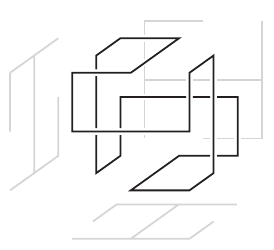
\includegraphics[scale=1]{pics/tree3}
\caption{Кривая три тени которой деревья.}
\label{pic:tree3}
\end{figure}

Кстати, эту головоломку теперь можно приобрести.
%ссылка не работает??? http://bitsandpieces.com/ˆBrainteasersˆMetal+Puzzles/07-W7871.html. 
Её придумал Оскар ван Девентер --- блестящий голландский изобретатель, чьи механические головоломки часто воплощают увлекательные математические идеи.

Так или иначе, Ленстра обратил внимание на то, что лабиринт на каждой грани коробки обязан быть деревом;
если бы он имел замкнутый цикл, то вывалилась бы часть пластика.
Тогда он задался вопросом, какова будет область доступных позиций для центральной точки трёх стержней.
Её проекция на каждую грань должна быть деревом, но может ли это множество само иметь цикл?
Если да, то такой цикл должен был проецироваться на каждую грань как дерево.
Так и возник вопрос.

Ленстра задумался над этим в феврале 1994 года, или около того.
Бергман расспрашивал об этом разных людей, но безуспешно.
Наконец, в сентябре 1995 года Кевин Базард, в то время постдок в Бёркли, сообщил Бергману и Ленстре, что вопрос был известен ещё раньше в Кембридже (Англия), и нашёлся пример.
Базарду этот пример показал Имре Лидер, комбинаторик из Кембриджского университета, который услышал о нём от Джона Рикарда, который его и придумал.
Тогда Рикард работал на математическом отделении Кембриджа, но теперь программист.

Пример Рикарда, который обладает очень красивой шестикратной симметрией, изображён на рис. \ref{pic:tree3}.

\subsubsection*{Игроки и победители}

Эта задача пришла ко мне от Алона Орлицкого из Университета Калифорнии в Сан-Диего.
Она иллюстрирует силу коммуникации \emph{от студента к учителю}.

Тристан и Изольда могут заранее пометить команды четырёхзначными двоичными кодами от 0000 до 1111 в алфавитном порядке.
Затем, когда Тристан узнает, кто играл, он может отправить Изольде 00, 01, 10 или 11 передав \emph{первую позицию в которой отличаются две метки команды} --- это может быть первый, второй, третий или четвёртый бит.
Изольде следует отправить обратно значение этого бита.

Например, если команда 0110 играла с командой 0011 и одержала победу,
то Тристан отправит Изольде «01», указывая, что метки играющих команд отличаются во втором бите.
Изольда отправит обратно «1» --- значение второго бита победившей команды.

Эта схема требует отправки трёх битов --- на один меньше, чем метод, при котором Изольда просто отправляет метку победившей команды.
Однако на самом деле этот бит обеспечивает экспоненциальное улучшение!
Если у нас $n = 2^{2^k}$ команд, то один метод требует $2^k$ битов, а другой всего $k + 1$.


\begin{addedbytheeditors}
 \textbf{Редакторам:} Возможно «от студента к учителю» надо переводить иначе.
Кто-нибудь владеет терминологией сложности коммуникаций?
 \end{addedbytheeditors}

\subsubsection*{Подсказка для Чарли}

На самом деле это серьёзная задача по сложности коммуникаций.
Она была рассмотрена Лесом Валиантом из Гарварда в 70-х годах,
а сообщил мне о ней Амит Чакрабарти из Дартмутского колледжа.
Решения этой и более общей задачи приведены в статье Павла Пудлака, Войтеха Рёдля и Йижи Шгалла \cite{49}.

Пусть $x_1, \dots , x_n$ --- биты, представляющие ответы, где (допустим) $1 = \text{«да»}$ и $0 = \text{«нет»}$.
Индексы берутся по модулю $n$.
Алиса отправляет Чарли $x_{-i}$,
а Боб отправляет Чарли все значения $x_a + x_b$ для всех пар $(a, b)$, таких что $a + b = j$ и $a\ne b$;
сумма битов берётся по модулю $2$.
Обратите внимание, что таких пар не больше чем $n/2$.

Чарли знает $x_{-i}$, а также $x_{-i} + x_{i+j}$, сложив их, он получит $x_{i+j}$.

Выглядит просто, но догадаться сложно.

\begin{addedbytheeditors}
\textbf{Редакторам:} Добавил $a\ne b$ и заменил не совсем верную фразу:
``Notice that there are n/2 such pairs (after rounding up
when n is odd).''
\end{addedbytheeditors}

\subsubsection*{Сближение по кривой}

Этим вопросом меня озадачил Оскар ван Девентер, тот, что уже упоминался выше.
Он думал использовать такую кривую в механической головоломке.
Такие кривые на самом деле существуют, сложнее найти пример для которого несложно доказать, что он не обладает вторым свойством.

На рис. \ref{pic:ss-curve} показана такая кривая, которую по своим причинам ван Девентер называет \emph{неконкинкульной}.
%non-conquinculous

\begin{figure}[htb!]
\centering
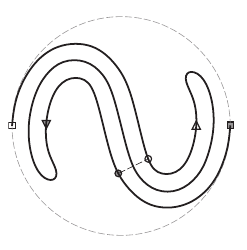
\includegraphics[scale=1]{pics/ss-curve}
\caption{Кривая со свойством (1), но без сойства (2).}
\label{pic:ss-curve}
\end{figure}

Пунктирная окружность на рисунке добавлена для того, чтобы было ясно, что кривая удовлетворяет первому свойству.
Остаётся убедиться, что для неё второе свойство не выполнено.
Предположим обратное, и пусть $t$ --- первый момент времени, когда один карандаш пройдёт от белого квадрата до белой стрелки,
либо же другой --- от серого квадрата до серой стрелки.
Какое-то время \emph{до} момента $t$ два карандаша окажутся друг напротив друга, как белый и серый круги.
Но \emph{после} времени $t$ им придётся разойтись, чтобы сойтись вместе, и это приведёт к увеличению расстояния.

Но как же догадаться до такой кривой?
(Если вопрос пугает, то пропустите следующие три абзаца.)
Представьте себе, что кривая параметризована параметром $t$;
это означает, что существует непрерывная функция $C$ из $[0, 1]$ в плоскость такая, что $C(0)$ --- один конец кривой (скажем, левый), $C(1)$ --- другой её конец, и $C(t)$ описывает кривую когда $t$ бежит от $0$ до $1$.
Успешное управление карандашами в соответствии со свойством (2) подразумевает пару непрерывных функций $f$ и $g$ из $[0,1]$ в себя, где в момент времени $t$ карандаши расположены в точках $C(f(t))$ и $C(g(t))$.
Таким образом, $f (0) = 0$, $g(0) = 1$, $f (1) = g(1)$, и расстояние от $C(f (t))$ до $C(g(t))$ не возрастает по $t$.
Вместе $f$ и $g$ описывают кривую от точки $(0,1)$ до линии $x = y$, в треугольнике с вершинами в $(0,1)$, $(0,0)$ и $(1,1)$.

Для того чтобы это стало невозможным, хотелось бы иметь \emph{двойственный путь} между прямыми $x = 0$ и $y = 1$, не выходящий на $x = y$, и соответствующий парам точек на локально минимальном расстоянии.
Такая кривая обязана пересечься с нашей кривой $(f, g)$, а это влечёт подъём расстояния.

Этот двойственный путь соответствует другому виду манипуляций с карандашами:
начинаем с левого карандаша в левой конечной точке и правого карандаша где-то на кривой,
затем перемещаем обе точки в одном направлении вдоль кривой, пока правый карандаш не достигнет правой конечной точки.
Если при этом ни одну точку нельзя переместить относительно другой без увеличения расстояния между ними, то мы достигли цели.
На данной фигуре карандаши начинают с белого квадрата и серой стрелки, затем движутся вместе, пока не достигнут белой стрелки и серого квадрата, соответственно.

\medskip

В награду за этот пример ваш автор получил прототип механической головоломки, замечательной как и все творения ван Девентера.

\subsubsection*{Суммы и произведения}

Эта забавная головоломка всплывала на различных формах в течение многих лет; она появилась в колонке Мартина Гарднера для Scientific American в декабре 1979 года, но по какой-то причине не вошла в сборник задач этой колонки \cite{29}.
Кажется удивительным, что столь туманной информации может хватить.

Головоломка (по сути, та же, что наша) была предложена независимо Стивом Феннером из Университета Южной Каролины и Биллом Готтесманом, разработчиком и производителем солнечных часов.
Ход рассуждений ниже предложен Готтесманом.

Для начала обозначим число Порфирио через $P$, а число Саманты через $S$, и пусть $\{X, Y\}$
--- неизвестная пара.
Вначале Порфирио не знает ответа, значит числа $X$ и $Y$ не могут быть оба простыми,
ни простым и его квадратом,
ни простым и его кубом.
Более того, ни одно из них не может быть большим простым числом (больше чем $50$), так как в этом случае оно должно было бы быть одним из сомножителей~$P$.

Следовательно, поскольку Саманта заранее знает, что Порфирио не может знать ответ,
$S$ не может превзойти $53$ или же быть равным сумме двух простых чисел.
Это исключает все чётные числа --- гипотеза Гольдбаха, проверенная далеко за $53$, гласит, что каждое чётное число больше $2$ представимо как сумма двух простых.
Остаются только некоторые из чисел, превышающие какое-то нечётное составное число на $2$, а именно
$11$, $17$, $23$, $27$, $29$, $35$, $37$, $41$, $47$ и $53$.
Готтесман назвал эти числа \emph{золотыми}.
(Например, $51=34+17$ и число $34\times 17$ допускает единственное разложение на сомножители до $100$.
Поэтому $51$ не золотое, хотя и превышает на $2$ составное число $49$.)
Не нужно беспокоиться о суммах простого числа и его квадрата или куба, так как они все чётные.

Из того, что Порфирио теперь уже знает $X$ и $Y$ (и из того, что сумма и произведение двух положительных целых чисел полностью их определяет), выводится, что множители всего одного разложения $P$ дают золотую сумму. 
Каждое золотое число $G$ даёт Саманте $(G - 3)/2$ возможных пар $\{X, Y\}$
(например, для $11$ можно собрать как $2 + 9$, $3 + 8$, $4 + 7$ или $5 + 6$); должно оказаться, что только одна из этих пар имеет произведение $P$ с желаемым свойством.

Если $G = 11$, то первые две пары выше уже позволяют Порфирио найти $X$ и $Y$.
Для случая $2 + 9$, получаем $P = 18$, и оно раскладывается только как $2 \times 9$ (где $2 + 9 = 11$ является золотым) или как $3 \times 6$ (дающее не золотую сумму $S = 9$).
В случае $3 + 8$ получаем $P = 24$, оно раскладывается как $2 \times 12$ (а $14=2+12$ не золотое) или
$3 \times 8$ (и $11=3+8$ золотое) или $4 \times 6$ (а $10=4+6$ не золотое).
Таким образом, $G$ не может быть $11$.

Следующее золотое число, $17$, подходит!
Ровно одна пара слагаемых даёт $P$, у которого единственная золотая сумма множителей равна $17$, а именно $4$ и $13$ (поскольку $2 + 26 = 28$, не золотое).

Надо ещё перебрать остальные шесть пар слагаемых для $17$, чтобы убедиться, что ни одна из них не даёт подходящего $P$.
Это даёт надежду, что $X$ и $Y$ могут быть $4$ и $13$.
Остаётся проверить, что $\{4, 13\}$ --- единственный ответ.
Для этого придётся повторить весь процесс для остальных восьми золотых чисел, 
и мы убедимся, что ни одно из них не подходит.

Решение этой головоломки не достаточно изящно,
хоть я и объявил это необходимым требованием (для решённых головоломок).
Однако то, что услышав этот короткий разговор, можно восстановить числа, не зная ни суммы, ни произведения, служит небольшим вознаграждением.

\begin{addedbytheeditors}
\textbf{Редакторам:}
Я не понял зачем говорить о квадратах и кубах.
И не понял почему не золотые 23 и 29.
(И нет охоты понимать.)
Почему там стоит 53? --- 53 это первое простое после 50, а числа начинаются с 2 --- вроде должно быть 54?
(Последнее конечно не влияет на рассуждение.) 

Кто-то должен это переписать.
\end{addedbytheeditors}

\subsubsection*{Сложенный многоугольник}

Эта головоломка пришла ко мне (как открытый вопрос) от Роберта Вейта из Юго-Восточного университета Индианы, который долго и тщетно пытался её решить.
Мне удалось найти (на мой взгляд) изящное решение, представленное ниже.
Позже выяснилось, что задачу уже решили К. Бёроцки, Г. Кертеша и Э. Макая \cite{9}.

Ответ такой: у каждого нечётноугольника с единчными сторонами площадь не меньше $\sqrt{3}/4$, причём равенство достигается только для треугольника.

Как такое доказывается?
Утверждение тривиально для треугольников,
и естественно возникает искушение воспользоваться индукцией по числу сторон.
Как мы увидим,  многоугольник с четырьмя и более сторонами разрезается диагональю на два многоугольника с меньшим числом сторон у каждого.
Однако, вообще говоря, новые многоугольники не будут равносторонними.
Таким образом, нужно придумать индукционное предположение применимое к более широкому классу многоугольников, возможно, ко \emph{всем}.

Приведённое ниже индукционное предположение отлично работает, хоть и выглядит топорно.
Важно правильно подобрать параметр.

Обозначим через $\mathbb{O}^n$ множество всех целочисленных $n$-векторов нечётного веса, то есть 
\[\mathbb{O}^n=\left\{\,\vec x=(x_1,\dots,x_n)\in \mathbb{Z}^n\,\middle|\, \sum_ix_i\equiv 1\pmod 2\,\right\}.\]
Чтобы измерить, насколько многоугольник $P$ близок к нечётноугольнику с единичными сторонами, мы воспользуемся параметром $u(P)$, назовём его \emph{нескладностью} $P$, определённым как
\[u(P)=1-\min_{\vec x\in \mathbb{O}^n} \left\{\sum_i |e_i-x_i|\right\}.\]
где  $e_1,\dots,e_n$ --- длины сторон $P$.
Заметим, что $u(P)\z\leqslant1$, и $u(P)\z=1$ если $P$ --- нечётноугольник с единичными сторонами или даже любой многоугольник с целочисленными сторонами и нечётным периметром.
С другой стороны, $u(P)\leqslant 0$ если, например, две из сторон многоугольника $P$ имеют длину $\tfrac12$, или же если у него чётный целый периметр.

Многоугольник будет считаться \emph{хорошим}, если у него нет вырожденных вершин,
то бишь нет вершин с внутренним углом $180\degree$.
Если $P$ имеет стороны длины больше~$1$, то из него можно получить (возможно нехороший) многоугольник $P^*$ со сторонами длины не более~$1$, подразбив каждую длинную сторону $P$.
При этом, можно добиться что бы $u(P^*)=u(P)$.

Теперь мы переходим к индукционному доказательству того, что площадь $A(P)$ любого многоугольника $P$ не меньше $\tfrac{\sqrt{3}}{4}u(P)$.
Отсюда немедленно последует, что площадь нечётноугольника с единичными сторонами не меньше  $\sqrt{3}/4$.

Ключ к доказательству --- \emph{субаддитивность} функции $u(P)$;
то бишь $u(P)\leqslant u(Q)+u(R)$, где $P$ --- многоугольник (возможно нехороший) и диагональ, скажем $D$, делит его на многоугольники $Q$ и~$R$.

Докажем субаддитивность.
Пусть  $e_1,\dots,e_n$ --- длины сторон $P$, а его диагональ $D$ имеет длину $d$. 
Выберем $\vec x\in\mathbb{O}^n$ такой, что $u(P)\z=1-\sum_i |e_i-x_i|$.

Пусть $I$ --- множество индексов сторон $P$, которые также являются сторонами $Q$, а $J$ --- индексы сторон $R$.
Обозначим через $\vec x|I$ и $\vec x|J$ сужение $\vec x$ на стороны (кроме диагонали) $Q$ и $R$ соответственно;
можно предположить, что $\vec x|I$ имеет нечётный вес.
Пусть $d_0$ --- ближайшее к $d$ чётное целое число, а $d_1$ --- ближайшее к $d$ нечётное целое число, так что $|d_1-d_0|=1$.

Взяв $\vec x|I$ вместе с $D$-координатой $d_0$ для $Q$ и 
$\vec x|J$ вместе с $D$-координатой $d_1$ для $R$, получим
\begin{align*}
u(R)+u(Q)
&\geqslant
1-\sum_{i\in I}|e_i-x_i|-|d_0-d|
+
1-\sum_{i\in J}|e_i-x_i|-|d_1-d|
=
\\
&=
2-\sum_{i}|e_i-x_i|-1=
\\
&=u(P),
\end{align*}
что и требовалось.

Теперь докажем главное утверждение для \emph{маленьких} треугольников.
А именно, если $T$ --- треугольник со сторонами не длинней $1$, то 
$A(T)\geqslant \tfrac{\sqrt{3}}{4}u(T)$.
Более того, равенство достигается только для равностороннего треугольника с единичными сторонами.

Пусть длины сторон треугольника равны $a$, $b$ и $c$.
Можно предположить, что целочисленный вектор, дающий $u(T)$, либо $(1, 0, 0)$, либо $(1, 1, 1)$.
Поскольку $a < b + c$, в первом случае имеем $u(T)\z=1-(1-a)-b-c<0$, и значит нечего доказывать.

Во втором случае
$u(T)=1-(1-a)-(1-b)-(1-c)=2s-2$, где $s=\tfrac12(a+b+c)$ --- полупериметр треугольника.
Можно считать, что $s > 1$, иначе опять нечего доказывать.
В частности, каждое из чисел $a+b$, $b+c$ и $c+a$ больше $1$.

Мы утверждаем, что при данном $s$, треугольник $T$ имеет наименьшую площадь если две из его сторон единичные (а третья, соответственно, длины $2s - 2$).

Дабы это увидеть, зафиксируем $a$. 
По формуле Герона (её красивое доказательство можно найти в \cite{39}) получаем
\[\frac{A(T)^2}{s(s-a)}=(s-b)(s-c)=s^2-(b+c)s+bc.\]
Поскольку сумма $b + c$ постоянна, минимум достигается, если $b = 1$ или $c = 1$.

Далее, переобозначив стороны, можно считать что $a = 1$.
Повторив рассуждение, получим уже две единичные стороны.
Иначе говоря, площадь $T$ не меньше площади треугольника со сторонами $1$, $1$, $2s - 2$, то есть \[\sqrt{s(s-1)(s-1)(2-s)}.\]

Поскольку $s\in(1,\tfrac32]$, получаем, что $s(2-s)\geqslant \tfrac34$.
Значит 
\[A(T)\ge \sqrt{\tfrac34(s-1)^2}=\tfrac{\sqrt{3}}2(s-1)=\tfrac{\sqrt{3}}4u(T),\]
и равенство достигается только при $s=\tfrac32$.

Перейдём к доказательству основного утверждения.
Предположим, оно неверно.
Тогда найдётся хороший многоугольник $P$ с минимальным числом сторон, скажем $n$, такой, что $A(P)<\tfrac{\sqrt{3}}4 u(P)$.
Если $n=3$, упорядочим треугольники лексикографически по ($\lceil c\rceil$, $\lceil b\rceil$, $\lceil a\rceil$), где 
$a\leqslant b\leqslant c$ --- длины сторон $P$, и потребуем, чтоб $P$ был минимальным в этом (частичном) порядке.

Предположим сначала, что $n>3$, и пусть $D$ --- любая внутренняя диагональ~$P$.
Такая диагональ найдётся, потому что если $P$ выпуклый, то любые две не соседние вершины соединяются отрезком внутри $P$.
В противном же случае есть вершина $v$ с внутренним углом больше $180\degree$.
Если отсканировать внутренность $P$ из $v$, начиная с направления одной из сторон при $v$ и заканчивая другой,
то мы увидим более чем одну из оставшихся сторон.
Там, где сканирование переходит от одной такой стороны к другой, мы увидим вершину, с которой и можно соединить $v$ диагональю.

Можно считать, что диагональ разбивает $P$ на хорошие многоугольники $Q$ и $R$, каждый с менее чем $n$ сторонами и, следовательно, каждый удовлетворяющий неравенству теоремы.
Но по субаддитивности, 
\[A(P)<u(P)\leqslant \tfrac{\sqrt{3}}4(u(Q)+u(R))\leqslant A(Q)+A(R)=A(P)\]
--- противоречие.

Остаётся рассмотреть случай $n=3$.
Пусть $A$ --- вершина противоположная стороне $a$, и так далее.
Из рассмотрения маленького треугольника, мы знаем что $\lceil c\rceil>1$.
Если $\lceil b\rceil<\lceil c\rceil$, проведём диагональ от $C$ к любой новой вершине $P^*$;
длина этой диагонали меньше, чем $b$, так как углы, прилегающие к длинной стороне, острые.
Оба треугольника, на которые эта диагональ разбивает $P^*$, лежат ниже $P$ в лексикографическом порядке.
Применив субаддитивность, приходим к противоречию.

В случае если $\lceil c\rceil=\lceil b\rceil>1$, выберем $P^*$ так, чтобы на стороне $b$ (соответственно на стороне $c$) на расстоянии $1$ от вершины $C$ (соответственно от вершины $B$) была новая вершина $U$ (соответственно $V$).
Проведём две диагонали, одну от $U$ к $V$% (длиной $d$)
, и другую от $V$ к $C$% (длиной $e$)
.
Снова, применив субаддитивность, заключаем, что один из трёх полученных треугольников $BCV$, $CVU$ и $VUA$, должен быть контрпримером.
Однако все эти треугольники предшествуют $P$ в лексикографическом порядке, и это противоречие завершает доказательство.

Остаётся заметить, что индукция, вместе со строгим неравенством для маленьких треугольников, влечёт строгость неравенства для любого хорошего многоугольника $P$, если только $P$ сам не равносторонний треугольник с единичными сторонами.

Уф!

\chapter{Не решённые и только-что решённые}


\setlength{\epigraphwidth}{.80\textwidth}
\epigraph{Мы должны знать --- мы узнаем!
}{--- Давид Гильберт (1862---1943)}

Плохая новость: эта глава может вас сломать.
Но есть и хорошая новость: нерешённая задача совсем не значит, что она неразрешима.
На самом деле две из нерешённых головоломок моей предыдущей книги были недавно решены.
Первая была особенно известной, и с ней произошло нечто поистине удивительное.

\section*{Ангел и дьявол Конвея}

Ангел летает над бесконечной шахматной доской и время от времени
должен садиться на клетку.
Он может пролететь не более 1000 ходов
короля до очередного приземления.

Пока ангел в небе, дьявол, живущий под доской, может уничтожить любую клетку на свой выбор.

Сможет ли дьявол добиться того, что ангелу некуда будет приземлиться?

\medskip

Поразительно и непостижимо, но эта открытая тридцать лет головоломка, была внезапно решена
независимо и почти одновременно
\emph{четырьмя} людьми из четырёх разных стран \cite{10, 20, 40, 43}.

При этом идеи были по большей части схожими, и они не опирались на недавно разработанные новые методы.
Более того, все доказательства строились на наблюдениях, сделанных самим Джоном Конвеем ещё в 70-х.
Четверо решивших были:
Андраш Мате из Университета имени Этвёша Лоранда в Будапеште,
Брайан Боудич из Университета Саутгемптона,
Оддвар Клостер из SINTEF ICT в Осло
и Питер Гакс из Бостонского университета.
Было давно известно, что ангела мощности $p=1$ (который перемещается на один ход короля) можно победить.
Мате и Клостер показали, что ангел мощности $p=2$ выигрывает;
Боудич доказал, что достаточно мощности $p=4$,
а Гакс --- что \emph{какой-то} мощности $p$ достаточно.

Доказательства оказались достаточно простыми, так что Бела Боллобаш из Кембриджского университета и Университета Мемфиса, смог разобрать их на восхитительном одночасовом докладе в Университете Иллинойса.
Далее следует выжимка из его доклада и статьи Мате, доказывающей, что ангел мощности 5 выигрывает.

Идея показать, что если ангел выигрывает (в несколько более сильном смысле) против несколько более слабого противника, называемого \emph{добрым дьяволом}, то он сможет выиграть и против изначального (\emph{злого}) дьявола.
Как мы увидим, против доброго дьявола сработает удивительно простая стратегия.

Доброму дьяволу запрещено уничтожать клетку, на которую ангел мог бы прыгнуть ранее;
другими словами, все клетки на расстоянии до $p$ от любой ранее посещённой ангелом клетки становятся недоступными.

Заметим, что ангел может выиграть в изначальной игре, если для любого $n$, он может уйти на расстояние $n$ ---
это легко проверить.
Мы хотим продемонстрировать, что если такое можно проделать с добрым дьяволом, то можно и со злым.

Предположим, у злого дьявола \emph{есть} стратегия, удерживающая ангела на расстоянии $n$ от начальной клетки.
Сейчас мы покажем, как добрый дьявол может сделать то же самое.
По данной последовательности ходов ангела, построим \emph{сокращённую} последовательность следующим образом.
Пусть $A_1$ --- самая ранняя клетка посещённая ангелом, с которой он мог бы прыгнуть на последнюю клетку $A_0$.
Удалим все ходы между $A_1$ и $A_0$.
Далее пусть $A_2$ --- самая ранняя клетка посещённая ангелом, с которой он мог бы прыгнуть прямо на~$A_1$.
Удалим все ходы между $A_2$ и $A_1$.
Продолжая таким образом, мы получаем сокращение $A_k$, $A_{k-1}, \dots, A_1$, $A_0$ исходной последовательности, в которой ангел никогда не прыгает в точку, с которой мог бы попасть ранее.

Теперь заставим доброго дьявола реагировать на данную последовательность ходов так, как это сделал бы злой дьявол в ответ на сокращённую последовательность, с одним изменением --- если требуется съесть недозволенную клетку (или нужная клетка уже съедена), то вместо этого добрый дьявол съедает любую дозволенную.
Легко показать, что если данная последовательность работает против доброго дьявола (то есть, ангелу не приходится сесть на съеденную клетку), то сокращение этой последовательности срабатывает против злого.
То есть, если ангел сможет уйти на расстояние $n$, играя против доброго дьявола, то он сможет сделать то же самое и против злого, а значит, сможет выиграть.

\begin{figure}[htb!]
\centering
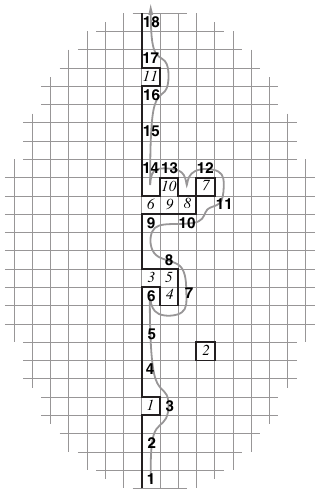
\includegraphics[scale=1]{pics/angel}
\caption{Стена отмечена чёрным, ангел --- жирным шрифтом, добрый дьявол --- курсивом.}
\label{pic:angel}
\end{figure}

Мы свели задачу к убеганию от доброго дьявола, а сделать последнее очень просто ---
ангел может даже позволить себе бегать, не прыгая, по несъеденным клеткам.
Он начинает на клетке, нижний левый угол которой находится в начале координат, и представляет себе стену вдоль линии $y = 0$.
Каждый раз, когда добрый дьявол съедает клетку, он возводит стену вокруг этой клетки.
Тем временем, на каждом ходу, ангел старается бежать на север вдоль стены, держа её слева от себя, пока это возможно.
Иногда ангелу придётся бежать на юг, чтобы обойти какой-то участок стены, но мощности $5$ 
хватает для того, чтобы продвигаться на север по крайней мере на единицу за каждый сделанный шаг.
Отсюда следует, что ангел мощности $5$ может уйти произвольно далеко.
Проделав дополнительную работу, можно убедиться, что и мощности $2$ достаточно.
На рис. \ref{pic:angel} показан возможный путь ангела мощности~$2$.

Стратегия ангела, описанная выше, конечно же \emph{не работает} против злого дьявола, который может, например, подготовить ловушку для ангела далеко по оси $y$ --- дьявол заманит ангела в конец полуострова, окружённого морем съеденных клеток, а затем отрежет его от берега.
Хороший дьявол не может этого сделать, ведь ему нельзя уничтожить вход на полуостров после того, как ангел туда прошёл.

К сожалению, то как стратегию убегания от доброго дьявола можно превратить в стратегию против злого, объяснить довольно трудно, даже при том, что построение выше довольно прямолинейно.
От части это и объясняет, почему головоломка оставалась так долго открытой, подтверждая при этом, что сокращения --- мощный инструмент.

\begin{addedbytheeditors}
\textbf{Редакторам:} Мутный оригинал и мутный перевод. Сам в доказательтве не разбирался, но может кому-то это интересно и этот кто-то всё перепишет?
\end{addedbytheeditors}


\medskip

Следующей головоломке ещё далеко до полного решения,
однако до недавнего времени про неё вовсе ничего не было доказано.

\section*{Затор}

Вершины бесконечной решётки на плоскости выбираются независимо с
фиксированной вероятностью $p\in (0,1)$.
В каждую из выбранных вершин
помещают автомобиль, направленный либо на север, либо на восток;
в каждом случае направление выбирается независимо подбрасыванием монеты.

Движение регулируется светофорами, которые включают поочерёдно:
«зелёный-восточный» и «зелёный-северный».
При включённом
зелёном-восточном каждый автомобиль, направленный на восток, правая
соседняя вершина от которого не занята, перемещается в эту вершину;
остальные (в том числе заблокированные другим восточным автомобилем),
остаются на месте.

Когда включается зелёный-северный, каждый незаблокированный
автомобиль, направленный на север, перемещается на одну вершину в
северном направлении.

Эксперименты показывают, что если $p$ меньше определённого
критического значения $p_0$, то автомобили постепенно разъедутся
(при этом каждый автомобиль будет иметь предельную скорость,
равную скорости автомобиля, который вовсе не блокируется).
Но когда
$p> p_0$, происходит обратное: автомобили попадают в безнадёжный
затор, то есть каждый автомобиль совершает лишь конечное число переездов
и останавливается навсегда.

Эту модель движения транспорта на перекрёстке двух крупных односторонних улиц представили О. Бихам, А. А. Миддлтон и Д. Левин в 1992 году \cite{6}.
Её странное поведение привлекло много внимания.
%библиографию можно найти по ссылке http://cui.unige.ch/spc/Bibliography/traffic.html.
%недоступная и незархивированя ссылка??? 

\begin{figure}[htb!]
\centering
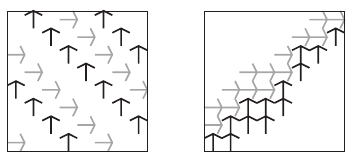
\includegraphics[scale=1]{pics/gridlock}
\caption{Свободное движение слева и затор справа.}
\label{pic:gridlock}
\end{figure}

На рис. \ref{pic:gridlock} изображены конечные части свободной конфигурации и конфигурации с затором, каждая из которых типична для того, что появлялось в экспериментах, проводимых Раисой Де Соуза \cite{15}, ныне преподаватель Университета Калифорнии в Дэвисе.

Весной 2005 года в Исследовательском институте математических наук в Бёркли Омер Ангел, Эндер Холройд и Джеймс Мартин сделали первый существенный шаг: они доказали существование фазы затора.
Другими словами, при достаточно высокой плотности машин произойдёт затор --- каждая машина совершит лишь конечное число переездов.
Мы не приводим доказательство, но оно весьма изобретательно использует теорию перколяций, и с ним очень стоит ознакомиться \cite{2}.

Конечно же, каждый раз, когда решается одна математическая задача, появляются три новые.
Думаю, что следующие несколько красавиц заслуживают внимания.

\subsection*{Упаковка прямоугольников}

Дан конечный набор точек в квадрате, включающий его нижний левый угол.
Разрешается выбрать набор непересекающихся прямоугольников, лежащих в квадрате, левые нижние вершины которых образуют данный набор точек.
Можно ли выбрать прямоугольники так, чтобы их общая площадь была не меньше половины площади всего квадрата?

\medskip

Эту сбивающую с толку задачу я узнал больше десяти лет назад,
о ней мне сообщил Билл Паллиблэнк (математик и администратор) из IBM, который не помнил, откуда она к нему попала.
С тех пор задача всплывала то там, то сям, но мне не удалось найти более ранний источник.
В июне 2004 года она появилась на веб-странице головоломок IBM \cite{ponder-this}, но так и осталась нерешённой.
Я даже не могу доказать то, что прямоугольники могут покрыть 1\% площади квадрата.

\begin{figure}[htb!]
\centering
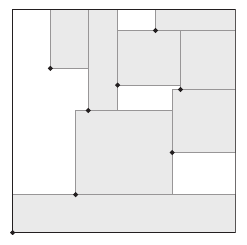
\includegraphics[scale=1]{pics/square}
\caption{Прямоугольники покрывают больше половины площади.}
\label{pic:square}
\end{figure}

На рис. \ref{pic:square} изображена конфигурация точек вместе с подходящим набором прямоугольников.

\subsection*{Произведения и суммы}

Можно ли раскрасить неотрицательные целые числа $\{0,1,2,\dots\}$ конечным числом цветов так, чтобы сумма $x+y$ и произведение $xy$ любых двух целых чисел были разных цветов?

\medskip

Эта задача была предложена Дэвидом Гэлвином, постдоком в Университете Пенсильвании.
Вроде как известен набор из шести чисел, таких, что любые два из них являются произведением и суммой некоторой пары, так что для раскраски потребуется по крайней мере шесть цветов.
С другой стороны, известно, что не существует произвольно больших наборов чисел с указанным свойством.

\medskip

Следующая загадка связана с игрой под названием «Социальное давление», придуманной Борисом Алексеевым из Университета Джорджии.
В неё активно играла команда США недавней математической олимпиады.

\subsection*{Социальное давление}

Двум игрокам сдают по некоторому числу карт, сначала \emph{в открытую} (рубашкой вниз).
На каждой карте написано целое число, все числа различны.
В каждом раунде игроки одновременно выкладывают по карте;
более высокая карта сбрасывается, а более низкая передаётся другому игроку.
Проигрывает тот у кого кончились карты.

При увеличении числа сдаваемых карт,
какова предельная вероятность того, что у одного из игроков будет выигрышная стратегия?

\begin{addedbytheeditors}
\textbf{Редакторам:} Не смог понять с чего игра называется peer pressure.
\end{addedbytheeditors}

\medskip

Борис (как и я) подозревает, что эта вероятность стремится к нулю, но анализ этой простой вариации игры в пьяницу кажется сложным.

\medskip

А вот неожиданная загадка от Стива Хедетниеми из Университета Клемсона:

\subsection*{Покрытие ферзями}

Пусть $f(n)$ --- минимальное число ферзей, которые можно расставить на доске размера $n \times n$ так, чтобы каждая клетка была под ферзём или под боем ферзя.
Верно ли, что $f(n + 1) \geqslant f(n)$ при всех $n$?

\medskip

Есть уйма головоломок о расстановке шахматных фигур (обычно ферзей или коней) на доске $n \times n$.
Для ферзей обычно стараются расставить как можно большее их число так, чтобы ни один не бил другого.
Однако нам нужно наименьшее число ферзей, контролирующих всю доску.
Трудно поверить, что для контроля меньшего числа клеток может понадобиться больше ферзей, однако на большей доске есть больше мест, откуда ферзь может контролировать свои владения, и это нужно учитывать!

\medskip

А вот увлекательная, но на самом деле довольно серьёзная головоломка, которая уже многие годы сбивает с толку специалистов по оптимизации.

\subsection*{Встреча}

Двое приятелей потеряли друг друга в огромном торговом центре. %???The Mall of America (аббревиатура: MOA, с англ. — «Молл Америки») — торговый центр, расположенный в Миннесоте в пригороде Миннеаполиса, неподалеку от аэропорта Миннеаполис/Сент-Пол. Он был открыт в 1992 году и является одним из крупнейших торговых центров мира.
На поиск в одном магазине у них уходит по 15 минут,
при этом время перемещения от одного магазина к другому ничтожно мало
(торговый центр --- удобно устроенный огромный многоэтажный квадрат).
Они не договорились о месте встречи и не определили заранее, кто будет искать, а кто останется на месте.
Как им следует действовать, чтобы минимизировать ожидаемое время поиска?

\medskip

Если один из них ищет, а другой ждёт на месте, то в среднем потребуется проверить $n/2$ магазинов, где $n$ --- число магазинов в торговом центре (предполагается, что оно большое).
Однако наши правила запрещают протокол, нарушающий симметрию;
нельзя, например, чтоб младший искал, а старший сидел на месте.
Если оба ищут, то в среднем потребуется $n$ шагов, до того как они окажутся в одном и том же магазине в одно и то же время и найдут друг-друга.

Этот вопрос был сформулирован (в других словах) в 1976 году Стивом Альперном из Лондонской школы экономики.
О нём и некоторых других вопросах можно почитать на веб-сайте Ричарда Вебера из Кембриджского университета \cite{weber}.
Вебер и Э. Дж. Андерсон предложили алгоритм, согласно которому каждый из приятелей бросает изогнутую монетку, решая с вероятностью около $0{,}2475$ оставаться на месте или же проверять магазины в случайном порядке,
и через каждые 15 минут, в случае неудачи, повторять процесс.
Это приводит к успеху в среднем за $0{,}8289n$ шагов, однако никто не смог доказать то, что это оптимально.

\begin{addedbytheeditors}
\textbf{Редакторам:} Добавил «через каждые 15 минут,»
\end{addedbytheeditors}


\subsection*{Подкрученный прямоугольник}

Вы, наверное знаете, что ленту Мёбиуса можно получить из длинной прямоугольной бумажной ленты,
склеив её концы с подкруткой на пол оборота.
А какой длины нужна полоса?
Иными словами, прямоугольник каких пропорций оптимален для склейки ленты Мёбиуса, без растяжения или сгибания?

Дмитрий Фукс и Сергей Табачников представили эту головоломку \cite[Лекция 14]{19} вместе с доказательством, что отношение длины к ширине не может быть меньше $\pi/2 \sim 1{,}57$, и примером для любого отношения больше $\sqrt{3} \sim 1{,}73$.
Однако точный ответ неизвестен.

\begin{addedbytheeditors}
Задача решена Ричардом Шварцем \cite{schwartz}; отношение обязано превосходить $\sqrt{3}$.
\end{addedbytheeditors}


\subsection*{Торговые автоматы}

Несколько торговых автоматов в местной игровой зоне работают случайным образом,
иногда выдавая много жевательных резинок за раз, а иногда не выдавая вообще ничего.
Однако в среднем каждый автомат выдаёт одну жевательную резинку за раз.
Какова максимально возможная вероятность того, что все $n$ автоматов за раз выдадут больше чем $n$ жевательных резинок?

\medskip

Эта головоломка (сформулированная в терминах независимых случайных переменных) принадлежит Ури Фейге из Microsoft Research.
Кажется оптимальным заставить каждый автомат выдавать $n + 1$ жевательную резинку с вероятностью $1/(n + 1)$,
а иначе ни одной.
В этом случае мы получим больше, чем $n$ жевательных резинок если хоть один автомат сработает.
Это происходит с вероятностью
\[1-(1-\tfrac1{n+1})^{n+1},\]
которая подходит к $1 - 1/e \sim 63\%$, при больших $n$.
Пока никто не придумал ничего лучшего.
Сам Фейге доказал, что вероятность получить более чем $n$ жевательных резинок не может превысить $12/13$.

Разве может такая задача быть трудной?

\subsection*{Круги на плоскости}

Дано множество открытых единичных кругов, которое тысячекратно покрывает плоскость;
то есть, каждая точка $\mathbb{R}^2$ покрывается как минимум тысячью кругами.
Докажите, что круги можно раскрасить в красный и синий цвета так,
чтобы красные и синие круги по отдельности покрывали всю плоскость.

\medskip

Янош Пах из Нью-Йоркского университета является создателем (и экспертом по) этой замечательной открытой задаче.
В своей статье \cite{46} он доказал, что для любого симметричного многоугольника $P$ и любого положительного целого числа $r$ существует число $k$, такое что любое $k$-кратное покрытие плоскости параллельными переносами $P$ можно разбить на $r$ покрытий.
Но если многоугольник заменить на круг, то даже при $r = 2$ неизвестно найдётся ли такое $k$.

Я считаю, что $k = 4$ должно хватить.
А вы, что скажете?


\appendix
\chapter{Послесловие}


\setlength{\epigraphwidth}{.83\textwidth}
\epigraph{Я надеюсь, что потомки благосклонно отнесутся ко мне не только за то, что я объяснил, но и за то, что я намеренно пропустил, дабы удовольствие открытия досталось другим.}{--- Рене Декарт (1596---1650), Геометрия}


Верите вы Декарту или нет, не стоит верить мне, если я скажу, что намеренно пропустил кое-что дабы вы нашли это сами.
Однако в мой задачник не попало \emph{ужасно много} отличных увлекательных головоломок, а ещё больше таких предстоит придумать.
Среди приведённых ссылок многие доступны онлайн; там эти головоломки стоит поискать,
и конечно вы можете придумать свои собственные.

Головоломки не замена математическому образованию, но они помогают запомнить идеи, которые вы выучили, а ещё развлекают и развивают ум.
Этот задачник преследует ещё и дополнительную цель:
помешать математической интуиции заниматься самолюбованием.

Во всяком случае, мне это помогает.

\begin{flushright}
Питер Уилкнер\\
28 февраля 2007
\end{flushright}

{
\small

\printindex

}

{

\sloppy

\printbibliography[heading=bibintoc]


\fussy

}

\newpage

{

\tableofcontents

}

\end{document}
